% Archived pre-W10 manuscript body. The submission source is main.tex.
\documentclass[aps,prx,reprint,floatfix,superscriptaddress]{revtex4-2}
\usepackage[T1]{fontenc}
\usepackage[utf8]{inputenc}
\usepackage{microtype}
\usepackage{amssymb,amsthm,mathtools}
\usepackage{bm}
\usepackage{booktabs}
\usepackage{multirow}
\usepackage{array}
\usepackage{longtable}
\usepackage{tabularx}
\usepackage{enumitem}
\usepackage{graphicx}
\usepackage{xcolor}
\usepackage{hyperref}
\usepackage[nameinlink,noabbrev]{cleveref}

% revtex4-2 4.2f's legacy array patch is incompatible with array 2.6n
% (TeX Live 2026); retain the package's native tabular implementation.
\makeatletter
\let\switch@array\relax
\makeatother

\newtheorem{definition}{Definition}
\newtheorem{theorem}{Theorem}
\newtheorem{corollary}{Corollary}
\newtheorem{proposition}{Proposition}
\newtheorem{lemma}{Lemma}
\newtheorem{remark}{Remark}
\newtheorem{assumption}{Assumption}

\newcommand{\diagres}{\mathcal{R}_{\mathrm{diag}}}
\newcommand{\pcharge}{\mathsf{prec}}
\newcommand{\Ftwo}{\mathbb{F}_2}
\DeclareMathOperator{\lcmop}{lcm}

% ---- Packing-family scaling values filled by the experiment pipeline;
% ---- see BUILD_PLAN_claude_code.md for the frozen protocol.
\newcommand{\TBD}[1]{\textcolor{red}{\textbf{[TBD: #1]}}}
\newcommand{\pkResultsSummary}{All five paths completed at $m=4$; semantic
UCC, \texttt{qiskit opt3}, staq rotation folding, and the phase-polynomial
reference also completed at $m=8,16,32,64$, while rebased TKET PauliSimp
returned \texttt{predicate\_error} at those four sizes because its output
fell outside the Hadamard-free symbolic-certificate predicate. Semantic UCC
and the phase-polynomial reference produced the same linear resource sequence,
from $25/21/8$ gates/depth/\texttt{cx} at $m=4$ to $385/321/128$ at $m=64$.
Among the completed external rows, \texttt{qiskit opt3} and staq produced
$17m$ and $10m$ output gates, respectively, as the $r m$ token stream grew.
Status outcomes are recorded separately and omitted from numerical curves.}

\begin{document}

\title{Representation as a Computational Resource in Quantum Compilation:
Approximate Recoverability Tradeoffs and Model-Specific Fault-Tolerant Consequences}

\author{Jinze Yang}
\affiliation{School of Physics, Xidian University, Xi'an 710071, China}

\author{Yangyang Li}
\email{yyli@xidian.edu.cn}
\affiliation{Key Laboratory of Intelligent Perception and Image Understanding of Ministry of Education of China,
Joint International Research Laboratory of Intelligent Perception and Computation,
International Research Center for Intelligent Perception and Computation,
Collaborative Innovation Center of Quantum Information of Shaanxi Province,
School of Artificial Intelligence, Xidian University, Xi'an 710071, China}

\author{Xiu-Hao Deng}
\email{dengxiuhao@iqasz.cn}
\affiliation{Shenzhen International Quantum Academy, Shenzhen 518048, China}
\affiliation{Shenzhen Branch, Hefei National Laboratory, Shenzhen, 518048, China}

\date{\today}

\begin{abstract}
The choice of circuit representation can alter both compiled quality and
downstream fault-tolerant cost for equivalent unitaries, yet the community
lacks a quantitative framework connecting representation to compiler
resources. We formalize approximate recoverability---the problem of
producing a short output within operator-distance tolerance
$\epsilon$ from a lowered flat representation---under a budget-explicit
compiler model whose bit-level cut budget explicitly serializes control,
store, window, parameter, and intermediate-representation channels,
including random-access IR/cache state, random seeds, dynamic-pass state,
and width-dependent addresses. We construct cyclic $K$-ary packing
families with $K=\Theta(1/\epsilon)$ and exact wraparound separation, and
lower them to $r$ round-major modular additive updates per generator; the
sum implements the semantic unitary while every individual update is
independent of the final coefficient under canonical sharing.  For a
randomized compiler with failure probability $\delta$, at most $p=p(m)$
forward passes, full crossing-state cap $S$, and expected output bits $A_p$
committed while scanning the first $r-1$ rounds, we prove the unified bounds
\begin{equation*}
 \overline B_{\mathrm{out}},\quad
 \overline A_p+(2p-1)S
 \ \geq\ (1-\delta)m\log_2K-h_2(\delta),
\end{equation*}
with the output statement applied separately to family-relative and
self-contained codes. A block hybrid attains compact family-relative output
with $S=O((m/p)\log(K+1))$, within a constant factor of the transcript
lower bound, while the semantic aggregate needs only logarithmic state.
The randomized family-relative output bound is matched up to framing by an
explicit abort-on-coin construction.  The earlier binary/$\mathbb Z_3$
one-pass theorem strengthens the zero-error cut message to
$\lceil m\log_2 3\rceil$ and is recovered as a special case. An exact-semantics
corollary retains the prior fixed-width final-output lower bounds.
Controlled validation on a complete matched-representation matrix
and four-qubit exact-semantics witnesses confirms the constructive side
against strong configured baselines.  The matrix crosses seven encodings
with five compilers, including TKET PauliSimp and PyZX full-reduce, over a
balanced sweep of $m,r,K$, support density, schedule, and five seeds.
An executable three-cut fixture validates the file-backed mapping from all
formal budget fields to measured bytes, and a revised event tracer is ready for
a compliant commitment--cross-cut campaign.  A
fixed-total-error grid-synthesis/surface-code run reports logical and physical
resources under one explicit model rather than a per-rotation proxy. We conclude that recoverability
should be treated as a controlled variable in compilation and resource
estimation, not as an implementation detail.
\end{abstract}
\maketitle


\section{Introduction}
\label{sec:introduction}

Fault-tolerant quantum computing promises scalable quantum advantage, but
realizing this promise requires accurate resource
estimation~\cite{fellous2023optimizing,watkins2024surfacecode}. Recent
studies have shown that resource estimates can vary by orders of magnitude
depending on compilation choices, yet the community lacks systematic
methods for understanding when and why equivalent circuits compile to
different resource costs.

The root cause is a representation problem. A high-level circuit describing
a commuting diagonal phase layer with $m$ generators can be compiled in at
least two qualitatively different ways. A \emph{semantic-first} pipeline
preserves the generator--coefficient structure, aggregates repeated
coefficients, and lowers the aggregate representative once. A
\emph{materialize-first} pipeline expands the same layer into a flat
target-basis instruction stream and then attempts to recover aggregate
structure from local patterns. Both pipelines produce correct unitaries,
but they expose very different resource profiles to downstream synthesis
and fault-tolerant estimation.

This representation dependence is well known anecdotally. Phase-polynomial
and Pauli-gadget methods~\cite{amy2014tdepth,nam2018automated,cowtan2020phase}
exploit algebraic structure before returning to a gate circuit.
ZX-calculus methods~\cite{duncan2020graph,kissinger2020reducing,kissinger2020pyzx}
provide a global representation in which phases can propagate and merge
beyond local syntax. Architecture-aware
compilers~\cite{martiel2022architecture} and full-stack
toolchains~\cite{watkins2024surfacecode} make representation choices that
propagate into physical resource estimates. What is missing is a
quantitative framework that isolates the effect of representation from
other compilation variables and connects it to model-specific
fault-tolerant cost.

We address this gap by formalizing \emph{approximate recoverability}:
given a target unitary $U$ and a fixed approximation tolerance $\epsilon$
in projective operator norm, what compiler resources are required to emit
an output within $\epsilon$ of $U$ from a lowered representation? The
contributions of this paper are:
\begin{enumerate}[leftmargin=1.5em]
    \item An approximate recoverability framework with a budget-explicit
    compiler model charging a unified bit-level cut budget
    $B_{\mathrm{cut}}=B_{\mathrm{control}}+B_{\mathrm{store}}+
    B_{\mathrm{window}}+B_{\mathrm{parameter}}+B_{\mathrm{IR}}$, together
    with a self-delimiting growing-width token codec and explicit charges
    for RAM/DAG/cache layout, dynamic passes, random seeds, output length,
    and approximation error
    (\cref{sec:framework}).
    \item A cyclic $K_\epsilon$-ary packing with exact wrap margin,
    $K_\epsilon=\Theta(1/\epsilon)$, and an $r$-round modular update
    representation in which no token determines the aggregate.  For
    randomized failure $\delta$, separate output-code bounds
    $\overline B_{\mathrm{rel}}^{\mathrm{out}},
    \overline B_{\mathrm{self}}^{\mathrm{out}}
    \geq(1-\delta)m\log_2K_\epsilon-h_2(\delta)$, and the explicit
    forward-pass frontier
    $\overline A_p+(2p-1)S\geq
    (1-\delta)m\log_2K_\epsilon-h_2(\delta)$.  A memory-capped block
    compiler reaches compact relative output with
    $S=O((m/p)\log(K_\epsilon+1))$, giving a constant-factor upper
    envelope; the older two-round $K=2,Q=3$ result retains its stronger
    zero-error one-pass constant
    (\cref{sec:packing,sec:reduction,sec:w1-unified-frontier}).
    \item A representation-aware recovery pipeline with bounded recognition
    of supported Pauli-rotation, phase-ladder/gadget, and preset semantic
    patterns, aggregation certificates, and fallback, together
    with a full seven-representation by five-compiler matrix isolating
    representation effects (\cref{sec:compiler,sec:validation}).
    \item Controlled validation showing that semantic-first aggregation
    achieves $B_{\mathrm{rel}}=m+O(\log m)$ and $G=O(m)$ on the witness
    family (with these measures kept separate), that the mechanism is confirmed by
    ablation, and a theorem-linked packing-family scaling experiment at
    growing $m$.  A revised event tracer emits committed bytes and every
    cut-budget field as verified files; the checked three-cut fixture tests
    that accounting path, while fixed-total-error staq synthesis and an explicit
    surface-code QRE report logical $T$, physical qubits, cycles, factories,
    runtime, and spacetime volume (\cref{sec:validation,sec:ft-consequences}).
\end{enumerate}

The prior version of this work established a
representation-dependent recoverability boundary for exact semantics on
fixed-width witness families. Those results---the final-output lower
bound for constant-budget finite-window transducers, the four-qubit
irrational-angle independent-Pauli witness, and the rational CP witness
with period $T=131040$---are retained here as an exact-semantics
corollary (\cref{cor:exact-semantics-corollary}). The primary asymptotic
axes are now the number of independent phase terms $m$ and the requested
approximation tolerance $\epsilon$; the output lower bound scales as
$m\log(1/\epsilon)$.


\section{Operational Setup}
\label{sec:setup}

We define the operational pipeline in four stages:
\emph{semantic input}, \emph{basis lowering}, \emph{recovery}, and
\emph{synthesis/resource estimation}.

\begin{definition}[Semantic input]
\label{def:semantic-input}
A semantic input is a circuit description $C_{\mathrm{sem}}$ in a
representation that preserves generator--coefficient structure. For a
commuting diagonal phase layer with $m$ independent generators
$P_1,\ldots,P_m$ and coefficients $\theta_1,\ldots,\theta_m$, the semantic
input has $O(m)$ records of the form $(P_j, \theta_j)$.
\end{definition}

\begin{definition}[Basis lowering]
\label{def:lowering}
Let $\mathcal{L}_B(\cdot)$ denote exact lowering into a fixed target basis
$B$. The lowered circuit $\mathcal{L}_B(C_{\mathrm{sem}})$ is a flat
instruction stream over $B$ implementing the same unitary up to global
phase. Lowering preserves unitary semantics but need not preserve the
generator--coefficient structure.
\end{definition}

\begin{definition}[Recovery]
\label{def:recovery}
A recovery procedure $\mathcal{R}$ takes a lowered circuit
$\mathcal{L}_B(C_{\mathrm{sem}})$ and produces an output circuit
$C_{\mathrm{out}}$ such that
$d_{\mathrm{proj}}(U(C_{\mathrm{out}}), U(C_{\mathrm{sem}})) \leq \epsilon$
under the projective operator norm $d_{\mathrm{proj}}$. The recovery is
\emph{representation-aware} if it reconstructs aggregate structure; it is
\emph{materialize-first} if it operates only on local patterns.
\end{definition}

\begin{definition}[Synthesis and resource estimation]
\label{def:synthesis}
A fault-tolerant synthesis procedure maps $C_{\mathrm{out}}$ to a
discrete-gate circuit over a fault-tolerant gate set (e.g., Clifford+$T$)
subject to a total error budget $\epsilon_{\mathrm{total}}$. A quantum
resource estimator (QRE) then reports logical $T$ count, magic-state
demand, physical qubits, cycles, and spacetime volume under specified
architecture assumptions.
\end{definition}

The central question is: for a fixed target unitary $U$ and fixed
$\epsilon$, how do the compiler resources required by $\mathcal{R}$
depend on whether $\mathcal{R}$ receives $C_{\mathrm{sem}}$ or
$\mathcal{L}_B(C_{\mathrm{sem}})$?


\section{Approximate Recoverability Framework}
\label{sec:framework}

\subsection{Approximate Distance and Recoverability}

\begin{definition}[Projective operator norm distance]
\label{def:proj-norm}
For unitaries $U, V$ on $n$ qubits,
\begin{equation}
\label{eq:proj-norm}
  d_{\mathrm{proj}}(U, V) = \inf_{\phi \in \mathbb{R}} \|U - e^{i\phi} V\|_{\mathrm{op}}.
\end{equation}
  
The infimum is attained because the circle $\{e^{i\phi}\}$ is compact and
$\|U - e^{i\phi}V\|_{\mathrm{op}}$ is continuous in $\phi$.
\end{definition}

The projective distance directly eliminates global phase and is used as
the primary correctness criterion below, \eqref{eq:proj-norm}.

\begin{lemma}[Unitary-channel diamond comparison]
\label{lem:diamond-comparison}
For the unitary channels
$\mathcal U(X)=UXU^\dagger$ and $\mathcal V(X)=VXV^\dagger$, define the
\emph{unnormalized} diamond distance
$d_\diamond(\mathcal U,\mathcal V)
:=\|\mathcal U-\mathcal V\|_\diamond\in[0,2]$.  Then
\begin{equation*}
 d_{\mathrm{proj}}(U,V)
 \leq d_\diamond(\mathcal U,\mathcal V)
 \leq 2d_{\mathrm{proj}}(U,V).
\end{equation*}
If the normalized convention
$\widetilde d_\diamond:=\tfrac12\|\mathcal U-\mathcal V\|_\diamond$ is used,
the corresponding explicit relation is
$\tfrac12d_{\mathrm{proj}}\leq\widetilde d_\diamond\leq
d_{\mathrm{proj}}$.
\end{lemma}

\begin{proof}
Let $\Theta\in[0,2\pi]$ be the length of a shortest closed arc containing
the spectrum of $U^\dagger V$.  Centering that arc by a global phase gives
\begin{equation*}
 d_{\mathrm{proj}}(U,V)=2\sin(\Theta/4).
\end{equation*}
The numerical-range formula for two unitary channels gives
\begin{equation*}
 d_\diamond(\mathcal U,\mathcal V)=
 \begin{cases}
  2\sin(\Theta/2),&0\leq\Theta\leq\pi,\\
  2,&\pi\leq\Theta\leq2\pi.
 \end{cases}
\end{equation*}
For $\Theta\leq\pi$, the ratio is $2\cos(\Theta/4)\in[\sqrt2,2]$;
for $\Theta\geq\pi$, one has
$d_{\mathrm{proj}}\in[\sqrt2,2]$ and $d_\diamond=2$.  The two inequalities
follow.
\end{proof}

Consequently, a projective packing with separation $s$ is also a diamond
packing with separation at least $s$.  Every lower bound below therefore
holds with the \emph{same numerical accuracy threshold} when correctness is
instead required as
$d_\diamond(\mathcal U(C_{\mathrm{out}}),\mathcal U)\leq\epsilon$.
Under the normalized convention, the same argument uses packing separation
$s/2$ and correctness threshold $\epsilon/2$.
Conversely, a projective-error upper bound $\epsilon$ implies diamond error
at most $2\epsilon$; the exact constructive upper bounds used here have zero
error in either metric.  No diamond packing conclusion is inferred from the
upper inequality alone.

\begin{definition}[$\epsilon$-approximate recoverability]
\label{def:approx-recoverability}
Fix $\epsilon > 0$. Given a target unitary $U$ presented as a lowered
circuit $\mathcal{L}_B(C_{\mathrm{sem}})$, the $\epsilon$-approximate
recoverability problem asks for an output $C_{\mathrm{out}}$ with
$d_{\mathrm{proj}}(U(C_{\mathrm{out}}), U) \leq \epsilon$, using compiler
resources charged by the model below.
\end{definition}

\subsection{Budget-Explicit Compiler Model}

We retain the fixed-width finite-window model only for the exact corollary
and use the following more general randomized, random-access model for the
growing-width approximate results.

\begin{definition}[Sparse formal-parameter serialization]
\label{def:parmodule}
Fix formal angle symbols $\theta_1,\ldots,\theta_M$.  A parameter is stored
in normalized sparse form
\begin{equation*}
\begin{gathered}
 \lambda=\displaystyle\sum_{\ell=1}^{s}c_\ell\theta_{j_\ell}
 +\dfrac{a}{d}\pi,\\
 j_1<\cdots<j_s,\quad c_\ell,a\in\mathbb Z,\quad d\geq1,
\end{gathered}
\end{equation*}
with zero coefficients omitted and $\gcd(a,d)=1$.  Let
$\mathsf{u}(z)$ and $\mathsf{s}(z)$ be fixed self-delimiting codes for
nonnegative and signed integers.  The executable parameter serialization is
\begin{equation}
\label{eq:precision-charge}
\begin{aligned}
 \mathsf{ser}_{\mathrm{par}}(\lambda)
 &=\mathsf{u}(s)\prod_{\ell=1}^{s}
   \bigl(\mathsf{u}(j_\ell)\mathsf{s}(c_\ell)\bigr)\\
 &\quad\cdot\mathsf{s}(a)\mathsf{u}(d),\\
 \pcharge(\lambda)&:=|\mathsf{ser}_{\mathrm{par}}(\lambda)|.
\end{aligned}
\end{equation}
Thus one nonzero formal coefficient costs $O(\log M)$ rather than
$\Omega(M)$ bits.  Qubit and generator locations are not part of this
parameter payload; they are serialized by the complete-token codec below.
\end{definition}

\begin{definition}[Width-aware complete-token codec]
\label{def:token-codec}
Fix a self-delimiting integer code $\mathsf u$, a signed variant
$\mathsf s$, a two-bit Pauli code $\mathsf p$, and a reserved record
terminator $\mathsf d$.  A token $\tau$ with gate-type ID $g$, arity $r$,
ordered operand qubits $q_1,\ldots,q_r$, sparse Pauli support
$\{(z_\ell,\sigma_\ell)\}_{\ell=1}^{s}$, and $k$ parameter slots is encoded
as
\begin{equation*}
\begin{aligned}
\mathsf{ser}_{\mathrm{tok}}(\tau)
={}&\mathsf u(g)\mathsf u(r)
  \prod_{i=1}^{r}\mathsf u(q_i)\;\mathsf u(s)
  \prod_{\ell=1}^{s}
    \bigl(\mathsf u(z_\ell)\mathsf p(\sigma_\ell)\bigr)\\
 &\cdot\mathsf u(k)
  \prod_{a=1}^{k}
    \bigl(\mathsf u(\mathrm{id}_a)
           \mathsf{ser}_{\mathrm{par}}(\lambda_a)\bigr)\mathsf d .
\end{aligned}
\end{equation*}
The zero values of $r,s,$ or $k$ are explicitly encoded, so the record is
executable and uniquely parseable without out-of-band arity, support, or
delimiter information.  Update, IR-node, and output records use the same
field order, with an opcode specifying which fields are active.

At growing width $n$, an arbitrary qubit or generator choice alone requires
$\lceil\log_2 n\rceil$ bits in any injective codec; the concrete codec above
uses $O(\log n)$ bits per listed address and $O(s\log n)$ bits for an
$s$-sparse Pauli support.  Consequently there is no width-independent
``structural cost per token.''  The literal bit strings
$\mathsf{ser}_{\mathrm{tok}}$ are charged wherever a token is live or
emitted.  Only when $n=n_0$ and a complete-token precision bound $q$ are
both fixed is the token set $\Gamma_{B,n_0}^{\leq q}$ finite; the
fixed-width exact-semantics statements abbreviate it as $\Gamma_B(q)$.
\end{definition}

\begin{definition}[Randomized dynamic-pass compiler and serialized cut budget]
\label{def:compiler}
A compiler $\mathcal A$ may use random-access RAM, stacks, hash tables,
caches, DAG/graph IRs, and intermediate tapes; it may also select a finite
number $p=p(I,\rho)$ of scans or passes dynamically from the input $I$ and
a finite random seed/tape $\rho$.  The external input is append-only on its
first exposure.  Any consumed prefix that remains available for a later
scan---whether through a file, memory mapping, spool, or cache---is live
compiler storage and is charged below.  The final output is write-once.
At every execution cut $c$, serialize a complete restart snapshot in five
disjoint fields:
\begin{itemize}[leftmargin=1.5em]
    \item $\mathsf{ser}_{\mathrm{control}}(c)$: format version, pass and
    finite-control IDs, dynamic pass count and termination/scheduling state,
    all input/output heads and emitted-prefix lengths, end flags, framing
    lengths, and the random seed/tape with its cursor;
    \item $\mathsf{ser}_{\mathrm{store}}(c)$: the persistent and ephemeral
    RAM, stacks, hash-table keys, bucket layout, cache contents and metadata,
    with parameter payloads and IR objects replaced by location tags;
    \item $\mathsf{ser}_{\mathrm{window}}(c)$: the ordered live read-window
    token structures, including the structural fields of
    \cref{def:token-codec} but excluding parameter payloads;
    \item $\mathsf{ser}_{\mathrm{parameter}}(c)$: the location-tagged
    concatenation of every live parameter payload in control, store, window,
    and IR, each encoded by \eqref{eq:precision-charge};
    \item $\mathsf{ser}_{\mathrm{IR}}(c)$: every other live intermediate
    tape/DAG/table object and every rereadable consumed-input block that can
    affect future execution, serialized by node opcode, the structural
    fields of \cref{def:token-codec}, edge endpoints, multiplicity, and
    object boundaries, but with parameter payloads omitted.
\end{itemize}
The corresponding bit-level budget is
\begin{equation}
\label{eq:info-budget}
\boxed{
\begin{aligned}
B_{\mathrm{cut}}(c)
&=B_{\mathrm{control}}(c)+B_{\mathrm{store}}(c)\\
&\quad+B_{\mathrm{window}}(c)+B_{\mathrm{parameter}}(c)
      +B_{\mathrm{IR}}(c).
\end{aligned}}
\end{equation}
where each summand is the literal bit length of the named serialization.
For a fixed run, $B_{\mathrm{cut}}$ is the maximum over its cuts.  For
randomized compilers we use the worst-input expected budget
\begin{equation}
\label{eq:expected-cut}
 \overline B_{\mathrm{cut}}(\mathcal A,\mathcal I)
 :=\max_{I\in\mathcal I}\mathbb E_\rho
       \bigl[\max_c B_{\mathrm{cut}}(c;I,\rho)\bigr].
\end{equation}
The previously named quantities are now
unambiguous bit measures:
$Q:=\max_c B_{\mathrm{parameter}}(c)$ and
$V:=\max_c B_{\mathrm{IR}}(c)$; no theorem below substitutes either one
for the total $B_{\mathrm{cut}}$.  The final output is write-once and is
charged separately by the output codes below.
\end{definition}

\begin{remark}[Model scope and escape channels]
\label{rem:escape-channels}
Equation~\eqref{eq:info-budget} charges all restart information, not only
the finite-control state.  In particular, a ZX graph, phase-polynomial
table, spilled update log, hash table, cache, random seed, or materialized
intermediate tape is serialized in the indicated field, and all coefficients
are serialized in $B_{\mathrm{parameter}}$.  Dynamic rescanning is allowed,
but the pass schedule, heads, and any rereadable old input are part of the
snapshot.  The five fields are disjoint by construction, so parameter bits
are not counted again as store, window, or IR structure.  A compiler may
escape a RAM-only workspace lower bound by materializing a large IR, but it
then pays the same bits in $B_{\mathrm{cut}}$.
\end{remark}

\begin{definition}[Three noninterchangeable output measures]
\label{def:info-budget-bits}
Fix two prefix-free, streaming binary codes.  The self-contained code
$E_{\mathrm{self}}$ serializes a target-basis circuit using gate opcodes,
all qubit/generator addresses, record delimiters, and sparse parameters
using \cref{def:token-codec}; it assumes no family dictionary.  For a public
packing-family dictionary
$\mathcal F_m=(m,P_1,\ldots,P_m,K_{\mathrm{pack}},\Delta,B)$, the conditional code
$E_{\mathrm{rel}}(\cdot\mid\mathcal F_m)$ has (i) an aggregate mode
consisting of a self-delimiting header and a packed
base-$K_{\mathrm{pack}}$ block of $m$
digits, (ii) a literal mode containing complete target-basis records, and
    (iii) an ordered-share mode whose header declares a split point and whose
fixed public schedule permits generator addresses to be omitted from its
residue slots.  Ordered-share slots still include their round boundary and
packed-block delimiters, and (iv) a $p$-block hybrid mode whose header
declares the pass blocks and passthrough coordinates and whose data section
contains packed aggregate blocks and round-major residue blocks in that
public order.  Define
\begin{equation}\label{eq:Bout-def}
\begin{aligned}
 B_{\mathrm{rel}}(C\mid\mathcal F_m)
 &:=|E_{\mathrm{rel}}(C\mid\mathcal F_m)|,\\
 B_{\mathrm{self}}(C)&:=|E_{\mathrm{self}}(C)|,\\
 G(C)&:=\text{number of target-basis gates in }C.
\end{aligned}
\end{equation}
For a compiler, a superscript ``out'' and a maximum over valid inputs denote
the worst-case output value of the corresponding measure; a barred
superscript ``out'' denotes the worst-input expectation over $\rho$.  These quantities
are not converted into one another: conditional description bits,
self-contained circuit bits, and gate count are reported and bounded
separately.
\end{definition}

\subsection{Executable Model--Implementation Correspondence}
\label{sec:model-implementation-mapping}

The formal fields above are implemented by one canonical binary codec rather
than by dimension-changing estimates.  The executable specification is
\texttt{encoding/FORMAT.md}; its reference implementation is
\texttt{encoding/codec.py}, and the only bit-accounting entry point is
\texttt{instrumentation/resource\_accounting.py}.  A complete codec frame has
the form
\begin{equation}
 \mathtt{UCCACCT0}\,\Vert\,
 \mathsf u(\text{version})\,\Vert\,
 \mathsf u(\text{type})\,\Vert\,
 \mathsf u(|z|)\,\Vert\,z,
 \label{eq:executable-codec-frame}
\end{equation}
where the displayed terminal zero denotes a null byte, $\mathsf u$ is the
canonical base-$128$ unsigned varint, and $z$ is a typed canonical payload.
Signed integers use zigzag coding; rational coefficients are reduced signed
numerator/positive-denominator pairs.  Maps are ordered by their UTF-8 key
bytes.  Qubit, generator, symbol, location, node, edge-endpoint, port, pass,
and head addresses are literal varints in $z$.

\begin{table*}[!t]
\centering
\scriptsize
\setlength{\tabcolsep}{3pt}
\begin{tabularx}{\textwidth}{@{}l l X X@{}}
\toprule
Formal object & Codec object/file & Included information & Measured field \\
\midrule
semantic input & \texttt{SemanticStream} & width and address-complete aggregate records & input artifact bits \\
dispersed flat input & \texttt{FlatUpdateStream} & width, round count, and every additive update & input artifact bits \\
$\mathsf{ser}_{\rm control}$ & \texttt{ControlState}/\texttt{control.uccbin} & pass count/index, heads, scheduling, status, framing and seed state when present & $B_{\rm control}$ \\
$\mathsf{ser}_{\rm store}$ & \texttt{StoreState}/\texttt{store.uccbin} & aggregate tables, maps, caches, stacks and their layout, excluding tagged parameter/IR payloads & $B_{\rm store}$ \\
$\mathsf{ser}_{\rm window}$ & \texttt{LiveWindow}/\texttt{window.uccbin} & ordered live complete-token structure and explicit parameter-slot count & $B_{\rm window}$ \\
$\mathsf{ser}_{\rm parameter}$ & \texttt{ParameterLedger}/\texttt{parameter.uccbin} & sparse symbolic parameters under complete location tuples & $B_{\rm parameter}$ \\
$\mathsf{ser}_{\rm IR}$ & \texttt{IRField}/\texttt{ir.uccbin} & serialized DAG width, opcodes, operands, nodes, edges, ports, boundaries and metadata, with parameters removed & $B_{\rm IR}$ \\
committed prefix & \texttt{committed-prefix.bin} & literal immutable prefix of a codec output frame & $B_{\rm com}$ \\
external output & \texttt{ExternalToolOutput} & tool, format and literal API payload & output artifact bits \\
certificate input & \texttt{CertificateInput} & certificate kind, certified-artifact SHA-256 and literal sidecar & certificate artifact bits \\
pass count & manifest \texttt{passes.count} and row \texttt{p} & actual declared scans of the instrumented compiler & $p$ \\
\bottomrule
\end{tabularx}
\caption{One-to-one map from formal serialized objects to executable artifacts.
No row permits a gate, token, support, or IR-node count to stand in for bits.}
\label{tab:model-implementation-map}
\end{table*}

\begin{lemma}[Canonical prefix-free implementation]
\label{lem:codec-prefix-free}
Version-one complete frames are injective and prefix-free.  Concatenations of
frames are uniquely parseable without an out-of-band arity or record count.
The semantic and flat decoders preserve their exact aggregate coefficient
table.
\end{lemma}

\begin{proof}
Canonical varints have a unique terminating byte, and the version, type, and
payload length are therefore uniquely decoded.  The declared payload length
locates the end of the frame.  A complete valid frame cannot be a proper prefix
of another complete valid frame: the shorter declared payload ends at its frame
boundary, whereas any following byte belongs to a subsequent frame.  Typed
payload values have distinct one-byte tags; lists and maps carry counts, maps
have strictly increasing keys, and reduced rational pairs are unique.  This
proves injectivity and unique concatenated parsing.  Finally,
\texttt{semantic\_signature} sums exact rational sparse parameters by the
literal pair (generator address, Pauli support), so encode--decode leaves the
aggregate table unchanged for both input representations.
\end{proof}

\begin{proposition}[File-backed accounting soundness]
\label{prop:file-backed-accounting}
Suppose the version-one verifier accepts a cut manifest $M$.  For every
$f\in\{\mathrm{control},\mathrm{store},\mathrm{window},
\mathrm{parameter},\mathrm{IR},\mathrm{com}\}$, let $A_f$ be the file named by
$M$.  Then the implementation reports
\begin{equation}
\begin{aligned}
 B_f&=8|A_f|_{\rm byte},\\
 B_{\rm cut}&=B_{\rm control}+B_{\rm store}+B_{\rm window}\\
             &\quad+B_{\rm parameter}+B_{\rm IR},
\end{aligned}
 \label{eq:file-backed-accounting}
\end{equation}
and reports the manifest pass count as $p$.  The reported values change when a
serialized address crosses a varint-width boundary.  They cannot be obtained
from a node or gate count alone.
\end{proposition}

\begin{proof}
The accountant first writes the five complete frames and the literal committed
prefix, then obtains every byte count by \texttt{stat}, stores the SHA-256 of
each file, writes $M$, and invokes the verifier before returning a row.  The
verifier reopens all six files, recomputes sizes and digests, decodes the five
restart fields, and rejects any disagreement.  It then forms the sum in
\eqref{eq:file-backed-accounting}; there is no count-to-bit code path.  Since an
address is a literal canonical varint, for example $127$ and $128$ occupy
different address lengths.  Conversely, two one-node DAGs may contain those
different addresses and hence have unequal file lengths despite equal node
count.
\end{proof}

\begin{remark}[Observable boundary versus restart cut]
\label{rem:observable-boundary-accounting}
The masked-share tracer serializes the five declared cut fields after every
update.  The verifier reopens and decodes every recorded field slice, checks
its size and digest, and recomputes the cut sum; its maximum is therefore a
file-backed measurement of the declared $B_{\rm cut}$ coordinate.  The W3
campaign does not claim that the Python process is destroyed and restarted
between events.  External compilers do not expose their private in-process DAGs,
caches, or tapes.  Their matched-matrix and natural-factorial rows consequently
report a file-backed \emph{API-boundary} snapshot and are diagnostic only; they
are not promoted to measurements of the maximum private $B_{\rm cut}$.  Peak
RSS remains a separate byte dimension and is not substituted for any field in
\eqref{eq:info-budget}.
\end{remark}

\begin{remark}[Self-contained and conditional descriptions]
\label{rem:dictionary-accounting-code}
Both input-stream objects declare either \texttt{self\_contained} or
\texttt{conditional}.  The former forbids an external dictionary.  The latter
requires the SHA-256 of the exact public family dictionary, and its manifest
records the dictionary's separate file size and whether it is charged at the
cut.  Thus a conditional description cannot silently be reported as a
self-contained circuit code.
\end{remark}


\subsection{Exact-Semantics Corollary from Prior Work}

We record the exact-semantics ($\epsilon = 0$) results
as corollaries; the full transducer proofs are
restated in \cref{app:sec:full-proofs}. The witness family is
fixed-width.

\begin{remark}[Separate fixed-width and growing-width encoding regimes]
\label{rem:encoding-regimes}
The exact corollary in this subsection fixes $n=n_0$, a precision bound
$q$, a deterministic constant pass count $p_0$, and one finite alphabet
$\Gamma_{B,n_0}^{\leq q}$; its unit is therefore a token over that fixed
alphabet.  No such constant-cost token assumption is made in the
growing-width results.  There $n=m+1$ (or $n\geq m$), the pass count may be
$p=p(m,I,\rho)$, and every input, output, RAM, and IR record is charged in
bits by \cref{def:token-codec} and \eqref{eq:info-budget}.
\end{remark}

\begin{definition}[Fixed-width witness family]
\label{def:witness-family}
Let $H_\Lambda$ be a fixed invertible boundary layer (a Hadamard layer in
the experiments) and let
$D = \prod_{j=1}^{m_0} \exp(-i\theta_j P_j/2)$
be a fixed commuting diagonal layer with Pauli-$Z$ characters
$P_j = Z^{a_j}$, $a_j \in \Ftwo^{n}$, and angles $\theta_j$. The witness
at repetition count $r$ is $C_r = H_\Lambda D^{r} H_\Lambda^{-1}$, with
exact lowering $\mathcal{L}_B(C_r) = \Pi M^r \Sigma$ for fixed token
strings $\Pi, M, \Sigma$.
\end{definition}

Two instances are certified and reused here. The
\emph{rational CP witness} ($n = 4$; ten $rz$/$cp$ terms;
$\operatorname{rank}_{\Ftwo}(A) = 4$) satisfies finite-range noncollision
with exact period $T = 131040$, certified by the self-contained rational
angle, single-term order, relative-phase, and LCM derivation in
\cref{app:sec:rational-period}. The
\emph{irrational independent-Pauli witness} ($n = 4$; supports
$1100, 0110, 0011, 1000$; $\theta_1/\pi = \sqrt{2}/11$) satisfies
unbounded noncollision by the following uniqueness lemma.

\begin{lemma}[Coefficient uniqueness for independent characters]
\label{lem:coeff-uniqueness}
If $a_1,\ldots,a_{m_0} \in \Ftwo^{n}$ are linearly independent and two
diagonal layers with coefficient vectors $\alpha, \alpha'$ satisfy
$D(\alpha) = e^{i\varphi} D(\alpha')$, then
$\alpha_j \equiv \alpha'_j \pmod{2\pi}$ for every $j$. In particular, if
some $\theta_j/\pi$ is irrational, the powers $D^{r}$ are pairwise
distinct up to global phase for all $r \geq 1$.
\end{lemma}

\begin{proof}
Independence makes
$z \mapsto (\chi_{a_1}(z),\ldots,\chi_{a_{m_0}}(z))$ surjective onto
$\{\pm 1\}^{m_0}$. Comparing the phase constraint at two sign patterns
that differ only in coordinate $j$ gives
$2(\alpha_j - \alpha'_j) \equiv 0 \pmod{4\pi}$. For the second claim,
$(r-r')\theta_j \in 2\pi\mathbb{Z}$ with $\theta_j/\pi$ irrational forces
$r = r'$.
\end{proof}

\begin{assumption}[Finite-range noncollision]
\label{ass:noncollision}
On a range $1 \leq r \leq R$, the powers $D^1,\ldots,D^R$ are pairwise
distinct up to global phase.
\end{assumption}

\begin{assumption}[Unbounded noncollision]
\label{ass:unbounded-noncollision}
The powers $D^r$, $r \geq 1$, are pairwise distinct up to global phase.
\end{assumption}

\begin{corollary}[Exact-semantics final-output lower bound]
\label{cor:exact-semantics-corollary}
\label{thm:final-output}
Assume exact lowering ($\epsilon = 0$), a fixed-width witness
$C_r = H_\Lambda D^r H_\Lambda^{-1}$ with
$\mathcal{L}_B(C_r) = \Pi M^r \Sigma$, and unbounded noncollision
(\cref{ass:unbounded-noncollision}). Let $\mathcal{A}$ be a uniform
deterministic finite-window, finite-burst transducer with constant budget
(constant $p,w,\mu$ and $B_{\mathrm{cut}}$) that is correct for every
$r \geq 1$. Then there exist constants
$h \geq 1$, $D \geq 1$ (depending on $\mathcal{A}$ and the witness but not
$r$) such that for every $r \geq h + D$,
\begin{equation}\label{eq:exact-output-bound}
  |T_p(r)| \geq \frac{r-h-D+1}{D} = \Omega_{\mathcal{A}}(r).
\end{equation}
\end{corollary}

\begin{proof}
This is \cref{app:thm:final-output}, proved in full in
\cref{app:sec:full-proofs}. Constant budget gives one finite
charged alphabet; per-tape pumpability propagation gives pumpability of the
final output; noncollision prevents collapse of distinct pump residues.
\end{proof}

\begin{corollary}[Finite-range tail form]
\label{cor:finite-tail}
Under finite-range noncollision (\cref{ass:noncollision}) with $N(R)=R$ on
$1 \leq r \leq R$, $|T_p(r)| \geq (r-h-D+1)/D$ for $h+D \leq r \leq R$.
For the rational CP witness, this applies only for $R < T = 131040$.
\end{corollary}

\begin{corollary}[Counting toll for short outputs]
\label{cor:counting-toll}
If finite-range noncollision supplies $N(R)$ distinct targets, then every
deterministic exact compiler satisfies
\begin{equation*}
 \max_{1\leq r\leq R}B_{\mathrm{self}}(T_p(r))
 \geq \left\lceil\log_2N(R)\right\rceil.
\end{equation*}
The same statement holds for $B_{\mathrm{rel}}(\cdot\mid\mathcal F)$
when one fixed public dictionary $\mathcal F$ is used on the entire range.
\end{corollary}

The irrational independent-Pauli witness instantiates
\cref{cor:exact-semantics-corollary} for all $r$ via
\cref{lem:coeff-uniqueness}; the rational CP witness instantiates
\cref{cor:finite-tail} on ranges $R < T$. These exact-semantics results
concern $\epsilon = 0$ and fixed width $n = 4$; the results below
generalize to growing $m$ and expose the dependence on $\epsilon>0$.


\section{Packing Construction}
\label{sec:packing}

\subsection{Growing-Width Family}

\begin{definition}[Packing family]
\label{def:packing-family}
For each $m$ and accuracy scale $\epsilon$, a packing family
$\mathcal F_{m,\epsilon}=\{U_x:x\in\mathcal X_{m,\epsilon}\}$ has
pairwise projective separation greater than $2\epsilon$, a semantic
description of $O(m)$ addressed records, and a lowered streaming
description whose aggregate information may be dispersed across updates.
The accuracy-dependent construction below has
$|\mathcal X_{m,\epsilon}|=K_\epsilon^m$ with
$K_\epsilon=\Theta(1/\epsilon)$.
\end{definition}

\begin{definition}[$K$-ary no-wrap construction]
\label{def:packing-construction}
Let $P_1,\ldots,P_m$ be $\Ftwo$-independent Pauli-$Z$ characters on $n \geq m$
qubits (i.e., $P_j = Z^{a_j}$ with $\operatorname{rank}_{\Ftwo}(a_1,\ldots,a_m)=m$).
Fix an integer $K\geq2$ and a step $\Delta>0$ satisfying
$(K-1)\Delta\leq\pi$.  Write $[K]_0=\{0,\ldots,K-1\}$.  For
$x\in[K]_0^m$, define
\begin{equation}\label{eq:Ux-def}
  \begin{aligned}
  U_x &= \exp\!\left(-\frac{i\Delta}{2}\sum_{j=1}^{m} x_j P_j\right) \\
      &= \prod_{j=1}^{m} \exp\!\left(-\frac{i\Delta x_j}{2} P_j\right).
\end{aligned}
\end{equation}
\end{definition}

\begin{lemma}[Packing separation]
\label{lem:packing-separation}
For the construction in \cref{def:packing-construction},
all $x\neq y\in[K]_0^m$ satisfy
\begin{equation}\label{eq:Kary-separation}
 d_{\mathrm{proj}}(U_x,U_y)\geq2\sin(\Delta/4).
\end{equation}
The constant is tight: pairs differing by one in a single coordinate
attain it.
\end{lemma}

\begin{proof}
Let $s=x-y$ and choose $j^*$ with $s_{j^*}\neq0$.
Since $P_j$ commute, $U_x U_y^\dagger = \exp(-\frac{i\Delta}{2}\sum_j s_j P_j)$
is diagonal in the computational basis. Its eigenvalue at basis state $z$ is
$\lambda(z) = \exp(-\frac{i\Delta}{2}\sum_j s_j \chi_{P_j}(z))$,
where $\chi_{P_j}(z) = (-1)^{a_j \cdot z} \in \{\pm 1\}$.

Because $a_1,\ldots,a_m$ are $\Ftwo$-independent, the map
$z \mapsto (\chi_{P_1}(z),\ldots,\chi_{P_m}(z))$ is surjective onto
$\{\pm 1\}^m$. Hence two basis states can be chosen whose character
vectors agree everywhere except at $j^*$.  Their eigenvalue arguments
differ by $\Delta s_{j^*}$ modulo $2\pi$.  The no-wrap condition gives
\begin{equation*}
 \Delta\leq |\Delta s_{j^*}|\leq(K-1)\Delta\leq\pi .
\end{equation*}

Now include the global-phase infimum required by
\cref{def:proj-norm}. For every $\phi \in \mathbb{R}$,
\begin{equation}\label{eq:packing-sep-norm}
\|U_x - e^{i\phi} U_y\|_{\mathrm{op}}
 = \max_z \bigl|\lambda(z)e^{-i\phi} - 1\bigr|
 \geq 2\sin(\Delta/4),
\end{equation}
because two points on the unit circle whose arguments differ by
$|\Delta s_{j^*}|\in[\Delta,\pi]$ cannot both lie within circular distance
less than $\Delta/2$ of $1$ after any common rotation, and
$|e^{i\gamma} - 1| = 2|\sin(\gamma/2)|$. Taking the infimum over $\phi$
preserves the bound. A one-coordinate difference of one has exactly two
spectral values separated by $\Delta$, and the centered choice of $\phi$
attains the lower bound.
\end{proof}

\begin{proposition}[$\epsilon$-tuned $K$-ary packing]
\label{prop:epsilon-packing}
For $0<\epsilon\leq1/8$, set
\begin{equation}\label{eq:epsilon-codebook}
\begin{aligned}
 L_\epsilon&=\left\lfloor
  \frac{\pi}{8\arcsin(2\epsilon)}\right\rfloor,&
 M_\epsilon&=4L_\epsilon,\\
 K_\epsilon&=L_\epsilon+1,&
 \Delta_\epsilon&=\frac{2\pi}{M_\epsilon}.
\end{aligned}
\end{equation}
Then $K_\epsilon=\Theta(1/\epsilon)$,
$(K_\epsilon-1)\Delta_\epsilon=\pi/2$ (so no coefficient wraps around
$2\pi$), and the $K_\epsilon^m$ targets in
\cref{def:packing-construction} obey
\begin{equation}\label{eq:epsilon-separation}
 d_{\mathrm{proj}}(U_x,U_y)
 \geq2\sin(\Delta_\epsilon/4)\geq4\epsilon
 \qquad(x\neq y).
\end{equation}
\end{proposition}

\begin{proof}
The restriction $\epsilon\leq1/8$ gives $L_\epsilon\geq1$.
Since $\arcsin(2\epsilon)=\Theta(\epsilon)$, the asserted order of
$K_\epsilon$ follows.  The equality in the no-wrap statement is direct.
Finally $L_\epsilon\leq\pi/(8\arcsin(2\epsilon))$, hence
$\Delta_\epsilon/4=\pi/(8L_\epsilon)\geq\arcsin(2\epsilon)$.
Apply \cref{lem:packing-separation} and monotonicity of sine on this range.
\end{proof}

\subsection{Streaming Encoding}

\begin{definition}[Balanced streaming encoding]
\label{def:streaming-encoding}
Fix the $K,\Delta$ of \cref{def:packing-construction}, a dispersal factor
$r$, and let $N = rm$. Let $\sigma : [N] \to [m]$ be
the round-robin schedule $\sigma(i) = ((i-1) \bmod m) + 1$, so that each
$j \in [m]$ has exactly $r$ preimages. For $x \in [K]_0^m$, define the
streaming encoding:
\begin{equation}\label{eq:streaming-W}
  W(x) = \prod_{i=1}^{N} R_{P_{\sigma(i)}}\!\left(\tfrac{x_{\sigma(i)} \Delta}{r}\right),
\end{equation}
where $R_{P_j}(\theta) = \exp(-i\theta P_j / 2)$.
\end{definition}

\begin{proposition}[Streaming encoding aggregates to $U_x$]
\label{prop:streaming-aggregates}
The product in \cref{def:streaming-encoding} equals $U_x$ exactly, since
the $P_j$ commute and each generator $P_j$ accumulates coefficient
$\sum_{i:\,\sigma(i)=j} \frac{x_j \Delta}{r} = x_j \Delta$.
\end{proposition}

\begin{definition}[Two-round masked-share lowering]
\label{def:masked-share}
Set the sharing modulus $K_{\mathrm{share}}=3$ and
$\alpha=2\pi/K_{\mathrm{share}}$.  The target packing and its aggregate
output code remain binary ($K_{\mathrm{pack}}=2$).  For every
$x\in\{0,1\}^m$, choose shares
$a^{(1)},a^{(2)}\in\mathbb Z_{K_{\mathrm{share}}}^m$ satisfying
\begin{equation}\label{eq:masked-share-W}
\begin{aligned}
 a_j^{(1)}+a_j^{(2)}&=x_j\pmod {K_{\mathrm{share}}},\\
 W_{\mathrm{MS}}(x;a^{(1)},a^{(2)})
 &:=\prod_{t=1}^{2}\prod_{j=1}^{m}
 R_{P_j}\!\left(\alpha a_j^{(t)}\right).
\end{aligned}
\end{equation}
The flat stream consists of records
$\mathsf{Update}(t,j,a_j^{(t)})$ in round-major order.  A record contains
the round tag, the full generator address $j$, and one residue in
$\mathbb Z_3$; it does not contain the aggregate $x_j$.  Indeed, for every
fixed first-round residue and either $x_j=0$ or $x_j=1$, a compatible
second-round residue exists.  Each residue has $O(1)$ parameter payload,
while a worst-case complete token has $\Theta(\log m)$ structural address
bits as required by \cref{def:token-codec}.
\end{definition}

\begin{proposition}[Masked shares aggregate projectively]
\label{prop:masked-aggregates}
Every valid stream in \cref{def:masked-share} implements $U_x$ up to global
phase.  In particular, no promise about either individual round is needed
for correctness.
\end{proposition}

\begin{proof}
Choose integer representatives of the residues.  For each $j$ there is an
integer $k_j$ with
$a_j^{(1)}+a_j^{(2)}=x_j+K_{\mathrm{share}}k_j$.  Commutativity and
$K_{\mathrm{share}}\alpha=2\pi$ give
\begin{equation*}
\begin{aligned}
 R_{P_j}(\alpha a_j^{(1)})R_{P_j}(\alpha a_j^{(2)})
 &=R_{P_j}(\alpha x_j+2\pi k_j)\\
 &=(-1)^{k_j}R_{P_j}(\alpha x_j).
\end{aligned}
\end{equation*}
Multiplying over $j$ changes only a global sign.
\end{proof}

\begin{remark}[Roles of the two flat schedules]
\label{rem:dispersal}
The balanced encoding of \cref{def:streaming-encoding} is retained only as
the configured experimental input in \cref{sec:validation}; because each
of its tokens contains $x_j/r$, it is not used to prove a representation
lower bound.  The theorem uses the masked-share stream instead.  Before the
second round arrives, every first-round update has two valid binary
aggregate completions, whereas the semantic representation supplies $x$
itself.  The separation below therefore charges recovery of an aggregate
hidden across rounds, not a voluntary delay after a full coefficient was
already visible.
\end{remark}


\section{Information Lower Bounds}
\label{sec:reduction}

We prove two lower bounds by one-way message arguments~\cite{kushilevitz1997communication}.
The first uses the $K_\epsilon^m$-point no-wrap packing and Fano's inequality
to obtain an explicit accuracy--description tradeoff, including randomized
compilers.  The second injects the $3^m$ possible first-round masks into the
message crossing the inter-round cut.  Its deterministic zero-error bound is
matched by a memory-capped hybrid compiler, and a conditional-Fano extension
covers randomized failure probability $\delta$.

\subsection{Packing Decoders}

\begin{lemma}[Nearest-packing decoder]
\label{lem:nearest-decoder}
Let $\mathcal F=\{U_x:x\in\mathcal X\}$ have pairwise distance at least
$4\epsilon$.  From any output circuit $C$, define
\begin{equation*}
 \widehat x(C)\in\arg\min_{y\in\mathcal X}
       d_{\mathrm{proj}}(U(C),U_y),
\end{equation*}
with a fixed tie rule.  If
$d_{\mathrm{proj}}(U(C),U_x)\leq\epsilon$, then $\widehat x(C)=x$.
\end{lemma}

\begin{proof}
The true target is at distance at most $\epsilon$.  Every other target is
at distance at least $4\epsilon-\epsilon=3\epsilon$ by the triangle
inequality, so it cannot minimize.
\end{proof}

The following binary-coordinate version will be used for the masked-share
tradeoff, where $K=3$ denotes the sharing modulus but the aggregate alphabet
remains $\{0,1\}$.

\begin{lemma}[Bit-class separation]
\label{lem:bit-class-separation}
For the binary subfamily of \cref{def:packing-construction}, put
$\epsilon_0=\sin(\Delta/4)$.  For each $i \in [m]$, partition the family into
$\mathcal{F}_i^{(0)} = \{U_x : x_i = 0\}$ and
$\mathcal{F}_i^{(1)} = \{U_x : x_i = 1\}$. Then the inter-class distance
satisfies
\begin{equation}\label{eq:bit-class-sep}
\operatorname{dist}\!\bigl(\mathcal{F}_i^{(0)},\,\mathcal{F}_i^{(1)}\bigr)
:= \inf_{\substack{x_i=0 \\ y_i=1}} d_{\mathrm{proj}}(U_x, U_y)
\;\geq\; 2\epsilon_0.
\end{equation}
\end{lemma}

\begin{proof}
Any pair with $x_i \neq y_i$ has $x \neq y$, so
\cref{lem:packing-separation} gives $d_{\mathrm{proj}}(U_x, U_y) \geq 2\epsilon_0$.
Taking the infimum preserves the inequality.
\end{proof}

\begin{lemma}[Representation-invariant decoder]
\label{lem:decoder}
For each $i \in [m]$ and any circuit $C$, define
\begin{equation}\label{eq:decoder}
\delta_i(C) :=
\arg\min_{b \in \{0,1\}}\ \min_{y:\, y_i = b} d_{\mathrm{proj}}(U(C), U_y).
\end{equation}
(Bob's local computation is unbounded, so he may exhaustively search the
$2^{m-1}$ candidates of each class.) If
$d_{\mathrm{proj}}(U(C_x), U_x) \leq \epsilon < \epsilon_0$, then
$\delta_i(C_x) = x_i$.
\end{lemma}

\begin{proof}
The correct class $b = x_i$ contains $U_x$ itself, so its inner minimum is
at most $\epsilon$. Suppose the wrong class $b \neq x_i$ also attained an
inner minimum $\leq \epsilon$, realized by some $U_y$ with $y_i = b$. Then
the triangle inequality gives
$d_{\mathrm{proj}}(U_x, U_y) \leq 2\epsilon < 2\epsilon_0$, contradicting
\cref{lem:bit-class-separation}. Hence only the correct class attains the
minimum, i.e.\ $\delta_i(C_x) = x_i$.
\end{proof}

\subsection{Output-Description Lower Bound}

\begin{theorem}[Randomized $\epsilon$--description tradeoff]
\label{thm:output-counting}
Let $0<\epsilon\leq1/8$, let $\mathcal F_{m,\epsilon}$ be the
$K_\epsilon$-ary family of \cref{prop:epsilon-packing}, and let a possibly
randomized compiler $\mathcal A$ output $C_{x,\rho}$ satisfying, for every
$x$,
\begin{equation}\label{eq:random-success}
 \Pr_\rho\!\left[
 d_{\mathrm{proj}}(U(C_{x,\rho}),U_x)\leq\epsilon
 \right]\geq1-\delta,
 \qquad 0\leq\delta<1/2.
\end{equation}
The compiler may use random-access RAM/DAG IR, hash tables, caches, and a
dynamic $p=p(m,x,\rho)$ as in \cref{def:compiler}.  Writing
$h_2(\delta)=-\delta\log_2\delta-(1-\delta)\log_2(1-\delta)$ with
$0\log 0:=0$, each output
code separately obeys
\begin{equation}\label{eq:output-counting}
\begin{aligned}
 \max_x\mathbb E_\rho
 B_{\mathrm{rel}}(C_{x,\rho}\mid\mathcal F_{m,\epsilon})
 &\geq(1-\delta)m\log_2K_\epsilon-h_2(\delta),\\
 \max_x\mathbb E_\rho B_{\mathrm{self}}(C_{x,\rho})
 &\geq(1-\delta)m\log_2K_\epsilon-h_2(\delta).
\end{aligned}
\end{equation}
In particular, for fixed $\delta<1/2$ both are
$\Omega(m\log(1/\epsilon))$.

At $\delta=0$, the family-relative bound is tight to lower-order framing
terms: a deterministic semantic compiler uses
\begin{equation}\label{eq:relative-epsilon-upper}
 B_{\mathrm{rel}}(C_x\mid\mathcal F_{m,\epsilon})
 \leq\lceil m\log_2K_\epsilon\rceil
       +O(\log m+\log K_\epsilon).
\end{equation}
Separately, for $P_j=Z_j$ and $RZ\in B$, the explicit self-contained
circuit satisfies
$B_{\mathrm{self}}(C_x)=O(m(\log m+\log K_\epsilon))$ and $G(C_x)\leq m$;
no self-contained-bit or gate-count tightness claim is made.
\end{theorem}

\begin{proof}
Let $X$ be uniform on $[K_\epsilon]_0^m$ and let $C=C_{X,\rho}$.
By \eqref{eq:epsilon-separation}, the nearest-packing decoder of
\cref{lem:nearest-decoder} has error probability at most $\delta$.  Fano's
inequality gives
\begin{equation*}
 H(X\mid C)\leq h_2(\delta)
       +\delta\log_2(K_\epsilon^m-1),
\end{equation*}
and hence
$I(X;C)\geq(1-\delta)m\log_2K_\epsilon-h_2(\delta)$.
For either prefix-free code $E$, source coding gives
$\mathbb E|E(C)|\geq H(C)\geq I(X;C)$.  The maximum conditional expected
length over $x$ is at least this uniform average, proving each line of
\eqref{eq:output-counting}.  This argument depends only on the output
distribution, so random access, dynamic passes, and internal IR do not
weaken it.

For \eqref{eq:relative-epsilon-upper}, the public dictionary supplies
$(P_1,\ldots,P_m,K_\epsilon,\Delta_\epsilon,B)$ and aggregate mode packs
the base-$K_\epsilon$ vector into one fixed-length integer block.  Its
header serializes $m,K_\epsilon$, the mode, and the block boundary.  In the
canonical self-contained construction, each nonzero $Z_j$ term has an
$O(\log m)$ address and an $O(\log K_\epsilon)$ rational-$\pi$ parameter
under \eqref{eq:precision-charge}; there are at most $m$ terms.
\end{proof}

\begin{corollary}[Deterministic fixed-grid specialization]
\label{cor:fixed-grid-output}
For any no-wrap $(K,\Delta)$ family of
\cref{def:packing-construction}, a deterministic compiler accurate to
$\epsilon<\sin(\Delta/4)$ has, separately,
\begin{equation*}
 B_{\mathrm{rel}}^{\mathrm{out}}\geq\left\lceil m\log_2K\right\rceil,
 \qquad
 B_{\mathrm{self}}^{\mathrm{out}}\geq\left\lceil m\log_2K\right\rceil.
\end{equation*}
In particular the binary fixed-step family has the $m$ line used in the
configured scaling panel.
\end{corollary}

\begin{proof}
Accuracy balls are disjoint by \cref{lem:packing-separation}, so the
deterministic output map is injective on $K^m$ inputs.  If $\ell_x$ are
their lengths under either prefix-free code, Kraft's inequality gives
$\sum_x2^{-\ell_x}\leq1$.  Thus
$K^m2^{-\max_x\ell_x}\leq1$, proving the two rounded bounds.
\end{proof}

\begin{remark}[What the counting bound does and does not say]
\label{rem:pass-through}
\Cref{eq:output-counting} holds regardless of internal resources, but the
two inequalities must not be cross-compared.  The packed $K_\epsilon$-ary
block in \eqref{eq:relative-epsilon-upper} is an upper bound only for
$B_{\mathrm{rel}}(\cdot\mid\mathcal F_{m,\epsilon})$; it is not a
self-contained target-basis circuit string.  Likewise $G(C)$ is never
multiplied by an implicit ``bits per gate'' constant.  The
representation-dependent question is addressed by the masked-share cut
below under one fixed family-relative output code.
\end{remark}

\subsection{The Masked-Share Compact-Output--Cut Tradeoff}

The semantic input supplies the aggregate vector $x$.  The flat input of
\cref{def:masked-share} instead supplies an arbitrary first share
$u\in\mathbb Z_3^m$ and only later a second share $v$ satisfying
$u+v=x\pmod 3$.  The cut between these rounds exposes information that is
specific to the representation: a correct compiler must preserve enough
about $u$ to handle every still-valid continuation $v$.

\begin{definition}[Masked-share cut and precommitted output]
\label{def:cuts}
Run $\mathcal A$ on a masked-share stream and let $c_{\mathrm{MS}}$ be the
arrival cut after all $m$ first-round updates have been delivered and before
any second-round update is available.  Before this cut the compiler may use
arbitrary RAM/DAG operations and a dynamic number of internal scans.  A
buffered or rereadable first-round record is included in
$B_{\mathrm{store}}$ or $B_{\mathrm{IR}}$; the only excluded prefix is one
irreversibly committed to the final write-once output.  Let
\begin{equation}\label{eq:Bcom-def}
\begin{aligned}
 B_{\mathrm{pre}}^{\mathrm{rel}}(\mathcal A,m\mid\mathcal F_m)
 &:=\max_{u\in\mathbb Z_3^m}
 \ell_{\mathrm{pre}}(u),\\
 B_{\mathrm{cut}}^{\mathrm{MS}}(\mathcal A,m)
 &:=\max_{u\in\mathbb Z_3^m}B_{\mathrm{cut}}(c_{\mathrm{MS}}(u)).
\end{aligned}
\end{equation}
Here $\ell_{\mathrm{pre}}(u)$ is the literal bit length already committed
under the prefix-monotone stream $E_{\mathrm{rel}}$; it is zero if final
output has not started.  Thus
$B_{\mathrm{pre}}^{\mathrm{rel}}\leq
B_{\mathrm{rel}}^{\mathrm{out}}$.
For randomized $\mathcal A$, barred quantities replace the maxima in
\eqref{eq:Bcom-def} by
$\max_u\mathbb E_\rho[\ell_{\mathrm{pre}}(u,\rho)]$ and
$\max_u\mathbb E_\rho[B_{\mathrm{cut}}(c_{\mathrm{MS}}(u,\rho))]$.
\end{definition}

\begin{theorem}[Representation-dependent masked-share tradeoff]
\label{thm:main-tradeoff}
Let the sharing modulus be $K_{\mathrm{share}}=3$, let $\alpha=2\pi/3$, and
$\epsilon_0=\sin(\pi/6)=1/2$.  Suppose first that a deterministic compiler
$\mathcal A$ is correct for \emph{every} valid two-round decomposition in
\cref{def:masked-share}:
\begin{equation*}
\begin{gathered}
 d_{\mathrm{proj}}(U(C(u,v)),U_{u+v\bmod 3})
 \leq\epsilon<\epsilon_0,\\
 u+v\bmod3\in\{0,1\}^m.
\end{gathered}
\end{equation*}
Then, under the single family-relative output code of
\cref{def:info-budget-bits},
\begin{equation}\label{eq:main-tradeoff}
 B_{\mathrm{pre}}^{\mathrm{rel}}(\mathcal A,m\mid\mathcal F_m)
 +B_{\mathrm{cut}}^{\mathrm{MS}}(\mathcal A,m)
 \geq \left\lceil m\log_2 3\right\rceil.
\end{equation}
Consequently, if the final output is family-relative compact,
\begin{equation*}
 B_{\mathrm{rel}}^{\mathrm{out}}(\mathcal A,m\mid\mathcal F_m)
 \leq m+c\log_2(m+2),
\end{equation*}
then
\begin{equation}\label{eq:compact-cut-floor}
 B_{\mathrm{cut}}^{\mathrm{MS}}(\mathcal A,m)
 \geq \left\lceil m\log_2 3\right\rceil
       -m-c\log_2(m+2)=\Omega(m).
\end{equation}
In contrast, a one-pass compiler receiving the semantic aggregate vector
$x$ streams the same aggregate-mode code with
$B_{\mathrm{rel}}^{\mathrm{out}}=m+O(\log m)$ and
$B_{\mathrm{cut}}=O(\log m)$.

More generally, let $0\leq\delta<1/2$ and let $\mathcal A$ be randomized
and satisfy the displayed
accuracy condition on every valid $(u,v)$ with probability at least
$1-\delta$.  It may use arbitrary random access and a dynamic
$p=p(m,u,v,\rho)$.  Then
\begin{equation}\label{eq:randomized-main-tradeoff}
 \overline B_{\mathrm{pre}}^{\mathrm{rel}}
 +\overline B_{\mathrm{cut}}^{\mathrm{MS}}
 \geq(1-\delta)m-h_2(\delta).
\end{equation}
In particular, for a deferred aggregate-mode compiler with
$\overline B_{\mathrm{pre}}^{\mathrm{rel}}=O(\log m)$ and fixed
$\delta<1/2$, the flat representation still requires
$\overline B_{\mathrm{cut}}^{\mathrm{MS}}=\Omega(m)$.
\end{theorem}

\begin{proof}
Let Alice hold an arbitrary first share $u\in\mathbb Z_3^m$.  She simulates
$\mathcal A$ through $c_{\mathrm{MS}}$ and sends the already committed
family-relative output prefix together with the complete five-field restart
serialization of \eqref{eq:info-budget}.  All head positions, lengths,
addresses, parameters, stores, windows, and materialized IR prefixes needed
to resume are present by definition, including any rereadable old input.
Bob, given a second share $v$, resumes the computation and runs its
dynamically chosen remaining operations locally.

The message must distinguish every pair $u\neq u'$.  To see this, choose a
single continuation $v$ coordinatewise.  If $u_j=u'_j$, set
$v_j=-u_j$.  If $u'_j=u_j+1\pmod3$, again set $v_j=-u_j$; the two aggregates
are then $0$ and $1$.  In the remaining case
$u_j=u'_j+1\pmod3$, set $v_j=-u'_j$; the aggregates are $1$ and $0$.
Thus both $(u,v)$ and $(u',v)$ are valid, binary aggregate instances, and
their aggregate vectors differ whenever $u\neq u'$.

If Alice's two messages were identical, determinism would make Bob emit the
same final circuit on these two valid completions.  That circuit cannot be
within $\epsilon$ of both targets, because
\cref{lem:packing-separation} gives target distance at least
$2\epsilon_0>2\epsilon$.  Hence the message map is injective on the
$3^m$ choices of $u$.  Serialize the restart snapshot first; its control
field gives the length of the committed prefix that follows, so the complete
messages are prefix-free.  Kraft's inequality therefore gives maximum
message length at least $\lceil m\log_2 3\rceil$.  The sum of the two
separate worst-case field lengths is at least that maximum, which proves
\eqref{eq:main-tradeoff}.  Prefix monotonicity and the assumed
upper bound on the final output give \eqref{eq:compact-cut-floor}.

For the semantic upper bound, the compiler writes the aggregate-mode header,
copies the arriving bits $x_j$ into the support-mask field, and retains only
a self-delimiting index and finite control.  It stores no coefficient table
or intermediate graph.  The sparse parameter payload is fixed and the live
address/index costs $O(\log m)$, so every cut has
$B_{\mathrm{cut}}=O(\log m)$ under the same serializer.

For the randomized extension, draw $U$ uniformly from $\mathbb Z_3^m$ and
$X$ uniformly from $\{0,1\}^m$, independently, and give Bob
$V=X-U\pmod3$.  Then $X$ and $V$ are independent and $H(X\mid V)=m$.
Alice's message $M$ consists of the committed prefix and the full restart
snapshot after processing $U$.  The snapshot includes the seed/tape and its
cursor, RAM, caches, old-input buffers, and IR, so Bob can resume the exact
randomized run upon receiving $V$.  The binary decoder of
\cref{lem:decoder} recovers $X$ with error at most $\delta$.  Conditional
Fano therefore gives
\begin{align*}
 H(X\mid M,V)&\leq h_2(\delta)+\delta m,\\
 I(X;M\mid V)&\geq(1-\delta)m-h_2(\delta).
\end{align*}
The two message fields are self-delimiting, so source coding lower-bounds
their expected total length by this conditional information, yielding
\eqref{eq:randomized-main-tradeoff}.  This is a conditional-Fano
(equivalently, distributional/Yao) argument and does not impose a fixed pass
count or sequential internal memory.
\end{proof}

\begin{proposition}[Memory-capped hybrid compilers]
\label{prop:hybrid-upper}
For every $\beta\in[0,1]$, let $h=\lfloor\beta m\rfloor$.  There is a
deterministic zero-error compiler for the masked-share stream, using the
ordered-share mode of $E_{\mathrm{rel}}$, such that at the inter-round cut
\begin{equation}\label{eq:hybrid-upper}
\begin{aligned}
 B_{\mathrm{cut}}^{\mathrm{MS}}
 &\leq h\log_2 3+O(\log m),\\
 B_{\mathrm{pre}}^{\mathrm{rel}}
 &\leq(m-h)\log_2 3+O(\log m).
\end{aligned}
\end{equation}
Thus \eqref{eq:main-tradeoff} is matched to leading order for every memory
fraction $\beta$ under this single family-relative encoding.  This statement
does not assert a matching curve for $B_{\mathrm{self}}$ or $G$.
\end{proposition}

\begin{proof}
The ordered-share header records $h$.  During round one the compiler packs
$u_1,\ldots,u_h$ into a base-three RAM block and immediately commits
$u_{h+1},\ldots,u_m$ in their public generator order.  It needs only the
packed block, an index, and framing state at the cut.  During round two it
emits the aggregates $u_j+v_j\pmod3$ for $j\leq h$ and the separate residues
$v_j$ for $j>h$.  The latter combine with the already emitted first shares;
all rotations commute, and \cref{prop:masked-aggregates} gives the target up
to global phase.  Fixed-order packing gives the two bounds in
\eqref{eq:hybrid-upper}; no qubit address is hidden, because the ordered-share
mode declares its public schedule and split in its header.
\end{proof}

\begin{corollary}[Compactness versus flat-share recovery]
\label{cor:output-inflation}
On the masked-share representation, any compiler with
$B_{\mathrm{cut}}^{\mathrm{MS}}=o(m)$ must have
\begin{equation*}
 B_{\mathrm{rel}}^{\mathrm{out}}(\mathcal A,m\mid\mathcal F_m)
 \geq m\log_2 3-o(m),
\end{equation*}
whereas family-relative optimal output $m+O(\log m)$ requires at least the linear
cut budget of \eqref{eq:compact-cut-floor}.  This is a representation
tradeoff: the semantic aggregate stream attains both compact output and
$O(\log m)$ cut budget.
\end{corollary}

\begin{proof}
Use $B_{\mathrm{pre}}^{\mathrm{rel}}\leq
B_{\mathrm{rel}}^{\mathrm{out}}$ in \eqref{eq:main-tradeoff}, then compare
with the semantic construction in \cref{thm:main-tradeoff}.
\end{proof}

\begin{remark}[Three points under one encoding]
\label{rem:corners}
All points in \eqref{eq:main-tradeoff} use
$E_{\mathrm{rel}}(\cdot\mid\mathcal F_m)$.  The semantic pass-through has
compact relative output and logarithmic cut budget.  A flat compiler that
materializes the first round in a table or intermediate graph pays its
full serialized structure and parameters in $B_{\mathrm{cut}}$.  A
one-pass flat compiler may instead commit update residues before seeing
their mates, but those records enlarge $B_{\mathrm{pre}}^{\mathrm{rel}}$
and hence the final relative code.  The hybrids of
\cref{prop:hybrid-upper} interpolate between these endpoints and attain the
deterministic lower envelope to leading order for every $\beta$.  No claim
about $B_{\mathrm{self}}$ or $G(C)$ is inferred from this curve.
\end{remark}

\begin{remark}[Relation to the exact-semantics results and model scope]
\label{rem:three-channels}
The exact-semantics corollary
(\cref{cor:exact-semantics-corollary}) bounds final output length under
exactness and noncollision, via pumpability.  \Cref{thm:output-counting}
bounds two explicitly named output-description codes via counting.
\Cref{thm:main-tradeoff} is different: it uses the two-round completion
adversary and the complete bit-level restart snapshot
$B_{\mathrm{cut}}$.  A global ZX graph, phase-polynomial table, spilled
store, large-precision parameter, addressed window, RAM/DAG, cache, hash
table, dynamic pass schedule, or random seed is therefore an accounted
recovery channel, not an exception.  The deterministic theorem allows
arbitrary $p=p(m,I)$ in this charged model, and
\eqref{eq:randomized-main-tradeoff} allows input-dependent randomized
$p=p(m,I,\rho)$.  The balanced experimental schedule is not claimed to
instantiate this lower bound.
\end{remark}


\section{Unified $K$-ary Randomized Multipass Frontier}
\label{sec:w1-unified-frontier}

The preceding results isolate output information and the binary two-round
cut.  The following package aligns the packing modulus with a genuinely
dispersed additive-update representation and makes the number of passes
and the full serialized state cap explicit.  It also separates the proved
constant-factor upper envelope from the remaining model-dependent gaps.

\subsection{Exact cyclic $K$-ary packing}
\label{sec:w1-qary-packing}

The no-wrap construction of \cref{def:packing-construction} is convenient
for output counting, but modular additive shares require a grid whose period
is also the sharing modulus.  The following formulation records exactly when
wraparound creates a collision.

\begin{definition}[Wrap margin]
\label{def:w1-wrap-margin}
For an alphabet $[K]_0$, step $\Delta>0$, and $K\geq2$, define
\begin{align}
 \operatorname{dist}_{2\pi}(a,0)
 &:=\min_{z\in\mathbb Z}|a-2\pi z|,\\
 \gamma(K,\Delta)
 &:=\min_{1\leq d\leq K-1}
       \operatorname{dist}_{2\pi}(d\Delta,0).
\end{align}
Let $P_1,\ldots,P_m$ be independent Pauli-$Z$ characters as in
\cref{def:packing-construction}, and set
\begin{equation}
 U_x^{(K,\Delta)}:=
 \exp\!\left[-\frac{i}{2}\sum_{j=1}^m x_j\Delta P_j\right],
 \qquad x\in[K]_0^m.
\end{equation}
\end{definition}

\begin{theorem}[Exact worst-pair separation]
\label{thm:w1-exact-separation}
For every $m\geq1$,
\begin{equation}
 \min_{x\neq y}d_{\mathrm{proj}}
 \bigl(U_x^{(K,\Delta)},U_y^{(K,\Delta)}\bigr)
 =2\sin\!\left(\frac{\gamma(K,\Delta)}4\right).
 \label{eq:w1-exact-separation}
\end{equation}
Consequently the family is projectively injective exactly when
$\gamma(K,\Delta)>0$.  If $(K-1)\Delta\leq\pi$, then
$\gamma(K,\Delta)=\Delta$.  If $Q\geq K+1$ and
$\Delta=2\pi/Q$, then again $\gamma(K,\Delta)=\Delta$, even though the
coefficient interval $[0,(K-1)\Delta]$ may cross the principal-argument
cut at $\pi$.
\end{theorem}

\begin{proof}
Fix $x\neq y$, put $s=x-y$, and choose $j$ with $s_j\neq0$.
Independence of the characters makes their joint sign map surjective.
Hence the relative unitary $U_x^{(K,\Delta)}
(U_y^{(K,\Delta)})^\dagger$ has two eigenvalues obtained from sign patterns
that agree off $j$ and whose circular angular separation is
$\operatorname{dist}_{2\pi}(|s_j|\Delta,0)\geq\gamma(K,\Delta)$.
After any common phase rotation, one of two circle points separated by
$\eta\in[0,\pi]$ is at chordal distance at least
$2\sin(\eta/4)$ from $1$.  This proves the lower bound in
\eqref{eq:w1-exact-separation} after taking the global-phase infimum.

Choose $d\in\{1,\ldots,K-1\}$ attaining $\gamma(K,\Delta)$ and take a pair that
differs by $d$ in one coordinate only.  Its relative spectrum consists of
two points with circular separation $\gamma(K,\Delta)$, so centering the
shorter arc attains $2\sin(\gamma/4)$.  This proves equality.  Under the
no-wrap hypothesis, every $d\Delta$ lies in $[\Delta,\pi]$, whose minimum
is $\Delta$.  For $\Delta=2\pi/Q$ and
$1\leq d\leq K-1\leq Q-2$, every nonzero grid distance is at least
$2\pi/Q$, with equality at $d=1$.
\end{proof}

\begin{corollary}[$\epsilon$-tuned cyclic family]
\label{cor:w1-epsilon-cyclic}
For $0<\epsilon\leq1/8$, let
\begin{equation}
 Q_\epsilon:=\left\lfloor
 \frac{\pi}{2\arcsin(2\epsilon)}\right\rfloor,
 \qquad K_\epsilon:=Q_\epsilon-1,
 \qquad \Delta_\epsilon:=\frac{2\pi}{Q_\epsilon}.
 \label{eq:w1-epsilon-grid}
\end{equation}
Then
\begin{equation}
 \frac1{4\epsilon}\leq K_\epsilon\leq\frac{\pi}{4\epsilon},
 \quad
 \min_{x\neq y}d_{\mathrm{proj}}(U_x,U_y)
 =2\sin\!\left(\frac{\pi}{2Q_\epsilon}\right)
 \geq4\epsilon.
 \label{eq:w1-epsilon-pack}
\end{equation}
Thus, with $\mathcal G_{m,\epsilon}:=
\{U_x:x\in[K_\epsilon]_0^m\}$,
\begin{equation}
 \log_2|\mathcal G_{m,\epsilon}|
 =m\log_2K_\epsilon
 =\Theta\!\left(m\log\frac1\epsilon\right).
 \label{eq:w1-packing-entropy}
\end{equation}
The allowed coefficient interval is
$[0,(Q_\epsilon-2)2\pi/Q_\epsilon]$.  It can extend beyond $\pi$ but
omits the residue $Q_\epsilon-1$; \cref{eq:w1-exact-separation}, rather
than a principal-interval argument, controls its wraparound.
\end{corollary}

\begin{proof}
The bound $\arcsin(2\epsilon)\leq\pi\epsilon$ and
$\lfloor a\rfloor\geq a-1$ give
$K_\epsilon\geq1/(2\epsilon)-2\geq1/(4\epsilon)$; the reverse bound uses
$\arcsin(2\epsilon)\geq2\epsilon$.  Since
$Q_\epsilon\leq\pi/[2\arcsin(2\epsilon)]$,
$\pi/(2Q_\epsilon)\geq\arcsin(2\epsilon)$.  Apply
\cref{thm:w1-exact-separation}.  The cardinality statement is immediate.
\end{proof}

\subsection{Dispersed additive-update representation}
\label{sec:w1-dispersed}

\begin{definition}[$r$-round dispersed update stream]
\label{def:w1-dispersed-stream}
The cyclic specialization of \cref{def:phase-family} with modulus
$Q\geq3$, $K=Q-1$, $\Delta=2\pi/Q$, $r\geq2$ rounds, and
$\Sigma=\{+1\}$: for $x\in[K]_0^m$ the shares
$a^{(1)},\ldots,a^{(r)}\in\mathbb Z_Q^m$ satisfy
\begin{equation}
 \sum_{t=1}^r a_j^{(t)}=x_j\pmod Q
 \qquad(j\in[m]),
 \label{eq:w1-share-sum}
\end{equation}
the flat input is the round-major record sequence
$\mathsf{Update}(t,j,a_j^{(t)})$, and the semantic input is the addressed
aggregate vector $x$.
\end{definition}

\begin{proposition}[Semantic equivalence and token privacy]
\label{prop:w1-stream-equivalence}
Every valid flat stream of \cref{def:w1-dispersed-stream} implements the
same $U_x$ as the semantic input, up to global phase.  Moreover, a single
flat token never determines $x_j$: for every fixed $(t,j,a)$ and every
$b\in[K]_0$, there is a valid stream with $a_j^{(t)}=a$ and $x_j=b$.
Under the canonical sharing distribution in which the first $r-1$ shares
are independent uniform residues and the last is fixed by
\eqref{eq:w1-share-sum}, every individual residue is uniform on
$\mathbb Z_Q$ and independent of $x_j$.
\end{proposition}

\begin{proof}
For integer representatives there are $k_j\in\mathbb Z$ with
$\sum_ta_j^{(t)}=x_j+Qk_j$.  Commutativity and $Q\Delta=2\pi$ give
\begin{equation*}
 \prod_tR_{P_j}(\Delta a_j^{(t)})
 =R_{P_j}(\Delta x_j+2\pi k_j)
 =(-1)^{k_j}R_{P_j}(\Delta x_j).
\end{equation*}
The product of the signs is global.  For privacy, fix the named token and
choose any one of the other $r-1$ residues to enforce the desired sum;
the remaining residues are arbitrary.  The distributional claim follows
because a sum containing at least one independent uniform residue is
uniform, including the last share after conditioning on $x_j$.
\end{proof}

\begin{definition}[Forward-pass cut accounting]
\label{def:w1-pass-accounting}
Partition the round-major stream into Alice's prefix $A$ (rounds
$1,\ldots,r-1$) and Bob's suffix $B$ (round $r$).  A forward $p$-pass
compiler scans $AB$ from left to right at most $p=p(m)$ times.  There are
$p$ crossings $A\to B$ and at most $p-1$ rewind crossings $B\to A$.
At every crossing, the complete restart state is the five-field
serialization of \eqref{eq:info-budget}; rereadable input and every live
IR object are therefore included.  For a run on $I$, let $A_p(I)$ be the
number of bits
irreversibly committed to the final output while the machine scans $A$,
summed over all passes, and define
\begin{equation}
 \Sigma_p(I):=\sum_{t=1}^{p}B_{\mathrm{cut}}(c_{A\to B,t})
       +\sum_{t=1}^{p-1}B_{\mathrm{cut}}(c_{B\to A,t}).
 \label{eq:w1-transcript-budget}
\end{equation}
Both are literal, self-delimiting transcript lengths.  Unbarred resource
symbols take maxima over valid inputs.  For randomized compilers, write
\begin{equation*}
 \overline A_p:=\max_I\mathbb E_\rho A_p(I,\rho),\qquad
 \overline\Sigma_p:=\max_I\mathbb E_\rho\Sigma_p(I,\rho),
\end{equation*}
and let
$S:=\max_I\mathbb E_\rho[\max_cB_{\mathrm{cut}}(c;I,\rho)]$ over the
$2p-1$ named crossings.  Then
$\overline\Sigma_p\leq(2p-1)S$; the deterministic version is identical
without expectations.
\end{definition}

\begin{theorem}[One-pass zero-error mask bound]
\label{thm:w1-one-pass-mask}
Let a deterministic one-pass compiler be correct to
$\epsilon<\sin(\pi/(2Q))$ on every valid stream of
\cref{def:w1-dispersed-stream}.  Then
\begin{equation}
 A_1+B_{\mathrm{cut}}(c_{A\to B,1})
 \geq\left\lceil m\log_2Q\right\rceil.
 \label{eq:w1-one-pass-mask}
\end{equation}
\end{theorem}

\begin{proof}
For each $u\in\mathbb Z_Q^m$, choose a canonical prefix whose aggregate
is $u$ (put $u$ in its first round and zero in the other prefix rounds).
The committed prefix and restart state after this prefix must distinguish
all $Q^m$ choices.  Indeed, for $u\neq u'$, choose one common final share
$v$ coordinatewise.  At each coordinate at most two residues of $v_j$
would make either $u_j+v_j$ or $u'_j+v_j$ equal to the single excluded
aggregate $Q-1$; since $Q\geq3$, an allowed $v_j$ exists.  Both completions
are valid, and they differ in every coordinate in which $u$ and $u'$ differ.
By \cref{thm:w1-exact-separation}, one circuit cannot be within
$\epsilon$ of both targets.  The messages are prefix-free under the
declared serializers, so Kraft's inequality gives
\eqref{eq:w1-one-pass-mask}.
\end{proof}

\subsection{Randomized multipass frontier}
\label{sec:w1-randomized-multipass}

Put
\begin{equation}
 L_\delta(m,K):=(1-\delta)m\log_2K-h_2(\delta),
 \qquad 0\leq\delta<\tfrac12.
 \label{eq:w1-Ldelta}
\end{equation}

\begin{theorem}[$K$-ary randomized multipass recoverability frontier]
\label{thm:w1-unified-frontier}
Let $Q\geq3$, $K=Q-1$, and
$0\leq\epsilon<\sin(\pi/(2Q))$.  Let a possibly randomized compiler be
correct within projective error $\epsilon$, with probability at least
$1-\delta$ for every $x\in[K]_0^m$ and every valid $r$-round dispersed
representation of $x$.  Assume that it makes at most $p=p(m)$ forward
passes in the charged model of \cref{def:w1-pass-accounting}.  Then:
\begin{align}
 \overline B_{\mathrm{rel}}^{\mathrm{out}}
 &\geq L_\delta(m,K),
 &
 \overline B_{\mathrm{self}}^{\mathrm{out}}
 &\geq L_\delta(m,K),
 \label{eq:w1-output-lower}\\
 \overline A_p+\overline\Sigma_p
 &\geq L_\delta(m,K).
 \label{eq:w1-pass-lower}
\end{align}
In particular, for the worst-input expected crossing cap $S$ of
\cref{def:w1-pass-accounting},
\begin{equation}
 \boxed{\quad
 \overline A_p+(2p-1)S
 \geq(1-\delta)m\log_2K-h_2(\delta).
 \quad}
 \label{eq:w1-frontier-box}
\end{equation}
Here $S$ includes RAM, parameters, cache/hash metadata, materialized input,
and all IR fields from \eqref{eq:info-budget}; it is not a RAM-only bound.
For the tuned choice of \cref{cor:w1-epsilon-cyclic}, both right-hand sides
are $\Omega((1-\delta)m\log(1/\epsilon))$ for fixed
$\delta<1/2$.
\end{theorem}

\begin{proof}
For \eqref{eq:w1-output-lower}, take $X$ uniform on $[K]_0^m$ and fix one
valid dispersed representation for each value of $X$.
The packing separation is greater than $2\epsilon$, so nearest-packing
decoding recovers $X$ from a successful output.  Fano's inequality gives
\begin{equation*}
 I(X;C)\geq m\log_2K-h_2(\delta)
 -\delta\log_2(K^m-1)\geq L_\delta(m,K).
\end{equation*}
Expected length in either separately fixed prefix-free output code is at
least this mutual information; a worst-input expectation is at least the
uniform average.

For \eqref{eq:w1-pass-lower}, independently choose a uniform prefix
aggregate $U\in\mathbb Z_Q^m$, put it in the first prefix round, put zero
in any other prefix rounds, and set the last share $V=X-U\pmod Q$.
Then $V$ is uniform and independent of $X$, so
$H(X\mid V)=m\log_2K$.  Convert the $p$ scans into the standard alternating
simulation across the $A\mid B$ partition.  The transcript $T$ contains
each complete crossing snapshot and all output chunks written on Alice's
side.  Given $T$ and $V$, Bob can reproduce every Bob-side segment and the
complete final output; random-tape state and dynamic control are present in
the crossing serialization.  The output decoder therefore recovers $X$
with error at most $\delta$, and conditional Fano yields
\begin{equation*}
 I(X;T\mid V)\geq L_\delta(m,K).
\end{equation*}
The framed transcript is prefix-free conditional on $V$, so its expected
literal length is at least this information.  Its length is precisely
$A_p+\Sigma_p$ up to fields already included in the self-delimiting
serializers.  Maximizing over inputs proves \eqref{eq:w1-pass-lower}; the
cap and tuned-$\epsilon$ consequences follow.
\end{proof}

\begin{remark}[What is and is not optimal]
\label{rem:w1-optimality-scope}
Equation~\eqref{eq:w1-output-lower} is an output-information bound and
\eqref{eq:w1-frontier-box} is a transcript bound; neither converts
self-contained circuit bits into gates.  The factor $2p-1$ counts the
actual alternating crossings of a forward scan.  A random-access input
oracle, an uncharged rereadable file, or reverse scans would be a different
model.  For $p=1$ and zero error, \cref{thm:w1-one-pass-mask} strengthens
$m\log_2K$ to $m\log_2(K+1)$.  No such strengthening is claimed for
randomized or general multipass protocols.
\end{remark}

\subsection{Memory-capped constructions}
\label{sec:w1-upper}

\begin{proposition}[Block hybrid]
\label{prop:w1-block-hybrid}
Fix $p,h\geq1$ and let $q=\min\{m,ph\}$.  There is a deterministic
zero-error $p$-pass compiler for \cref{def:w1-dispersed-stream} that
aggregates $q$ coordinates and passes the other update records through in
the public $p$-block hybrid mode of $E_{\mathrm{rel}}$.  It obeys
\begin{align}
 S&\leq \left\lceil\frac qp\right\rceil\log_2Q
       +O(\log(mQrp)),
 \label{eq:w1-upper-state}\\
 A_p&\leq(r-1)(m-q)\log_2Q+O(r\log(mQrp)),
 \label{eq:w1-upper-A}\\
 B_{\mathrm{rel}}^{\mathrm{out}}
 &\leq q\log_2K+r(m-q)\log_2Q
       +O(r\log(mQrp)).
 \label{eq:w1-upper-output}
\end{align}
In the compact-output corner $h=\lceil m/p\rceil$, this becomes
\begin{align}
 B_{\mathrm{rel}}^{\mathrm{out}}
 &\leq m\log_2K+O(\log(mQrp)),\\
 S&\leq\left\lceil\frac mp\right\rceil\log_2Q
       +O(\log(mQrp)).
 \label{eq:w1-compact-upper}
\end{align}
For two rounds, the construction satisfies
$A_p+pS\leq m\log_2Q+O(p\log(mQrp))$ after using a smaller final block.
Compared with
\eqref{eq:w1-frontier-box} at $\delta=0$, it is within the constant
$(2p-1)\log_2(K+1)/(p\log_2K)<2\log_2 3$ for every $K\geq2$.
\end{proposition}

\begin{proof}
Partition the first $q$ coordinates into at most $p$ consecutive blocks of
size at most $h$.  On pass $t$, keep only the residues of block $t$ and add
their first $r-1$ rounds modulo $Q$; when the final-round mates arrive,
emit the corresponding aggregate base-$K$ block.  The live packed block,
indices, and framing give \eqref{eq:w1-upper-state}.  On the first pass,
emit every share of each unselected coordinate in the declared round-major
order; these rotations already have the correct product and require no
retained coefficient table.  The selected coordinates can be balanced
across the $p$ blocks, so the maximum block has size $\lceil q/p\rceil$.
Their consecutive boundaries are a public function of $(m,p,q)$, so the
header stores those integers rather than $p$ separate delimiters.
The prefix contains $r-1$ residues and the
whole output contains $r$ residues for each such coordinate, giving
\eqref{eq:w1-upper-A} and \eqref{eq:w1-upper-output}.  If $ph\geq m$ there
are no passthrough coordinates.  For $r=2$, $(m-q)\log_2Q+ph\log_2Q$ is
at most $m\log_2Q$ up to the last partial block and framing.  The constant
comparison uses $(2p-1)/p<2$ and
$\log_2(K+1)/\log_2K\leq\log_2 3$.
\end{proof}

\begin{proposition}[Semantic and randomized upper corners]
\label{prop:w1-semantic-upper}
Under the same public dictionary, a one-pass semantic compiler receiving
$x$ emits the packed base-$K$ aggregate code with
\begin{equation}
 B_{\mathrm{rel}}^{\mathrm{out}}
 \leq\lceil m\log_2K\rceil+O(\log(mK)),
 \qquad S=O(\log(mK)),
 \label{eq:w1-semantic-upper}
\end{equation}
and implements the same $U_x$ as the flat stream.  For any
$0\leq\delta<1/2$, an input-independent abort coin that runs this exact
compiler with probability $1-\delta$ and otherwise emits a fixed short
circuit has worst-input success at least $1-\delta$ and expected relative
output
\begin{equation}
 (1-\delta)\lceil m\log_2K\rceil+O(\log(mK)+1).
 \label{eq:w1-random-upper}
\end{equation}
Thus the randomized family-relative output lower bound is matched up to
framing and the binary-entropy additive term.  A self-contained
$R_Z$-circuit upper bound remains
$O(m(\log m+\log Q))$ bits and at most $m$ rotations; no matching
self-contained-bit or gate-count claim is made.
\end{proposition}

\begin{proof}
Pack the ordered aggregate vector as one base-$K$ integer and retain only
its streaming index and framing state.  Proposition~\ref{prop:w1-stream-equivalence}
gives semantic equality with the flat representation.  Prefix the output
with the abort-coin branch tag for the randomized construction and take
expectations.  The self-contained construction writes each nonzero
$R_{P_j}(2\pi x_j/Q)$ with its address and rational parameter.
\end{proof}



\section{Representation-Aware Compiler}
\label{sec:compiler}

\subsection{Bounded Supported-Pattern Recognition}

\begin{definition}[Supported-pattern region recognizer]
\label{def:region-discovery}
The implemented recognizer accepts only configured high-level forms:
(i) explicit Pauli rotations or phase-gadget records that already carry
their support, (ii) local phase-ladder/Fourier spans, (iii) expanded
mirrored or self-inverse composite blocks, and (iv) repeated-run or preset
semantic nodes.  Within one supported contiguous span it maintains the
declared generators $P_1,\ldots,P_k$, coefficients
$\theta_1,\ldots,\theta_k$, qubit support, and source records.  It may extend
the span while the next record belongs to the supported grammar and passes
the configured commutation check; an unsupported or certified
noncommuting record closes the candidate.  Rejected recognition leaves the
original circuit available to the conservative fallback.
\end{definition}

\begin{remark}[Recognition, maximality, soundness, and complexity scope]
\label{rem:discovery-scope}
The artifact does not implement a general binary-symplectic extractor for
arbitrary circuit DAGs and does not claim a maximal commuting region in
that sense.  Its only maximality notion is the maximal contiguous span
accepted by the fixed supported-pattern grammar under the chosen scan
order.  Different generators remain separate records until aggregation.
Soundness of a selected rewrite comes from the independent exact or
symbolic equivalence certificate of \cref{def:certificate}; failure returns
the unchanged candidate.  No general worst-case linear-time claim is made:
the runtime is the sum of the bounded scans, signature/hash bookkeeping,
certificate work, and any configured backend probes, as detailed in
Appendix~B.
\end{remark}

\subsection{Aggregation and Certificate}

\begin{definition}[Aggregation of an accepted supported region]
\label{def:aggregation}
Given an accepted supported region with generators $P_1,\ldots,P_k$ and coefficients
$\theta_1,\ldots,\theta_k$, the aggregation emits a representative
circuit implementing $\exp(-i\sum_j \theta_j P_j / 2)$ using at most
$c_0 + c_1 k$ gates in the target basis.
\end{definition}

% W6: exact symbolic correctness certificate and soundness domain.
% This file is input by PaperDraft/ucc_v7_2_prxq_repaired/main.tex.

Let


\begin{equation*}
 \mathcal C_n=\langle H,S,S^\dagger,X,Y,Z,\mathrm{CX},
 \mathrm{CZ},\mathrm{SWAP}\rangle
\end{equation*}
be the Clifford gate language on addressed qubits.  Fix a declared finite
formal-symbol set $\mathcal S$ and the exact coefficient module
\begin{equation*}
 \Lambda=\mathbb Q\pi\oplus
 \bigoplus_{s\in\mathcal S}\mathbb Q\theta_s.
\end{equation*}
For a signed Hermitian $n$-qubit Pauli $P$ and $\lambda\in\Lambda$, write
$R_P(\lambda)=\exp(-i\lambda P/2)$.

\begin{definition}[Exact commuting-Pauli/Clifford certificate domain]
\label{def:certificate}
The domain $\mathcal D_{\rm CPC}$ consists of finite addressed circuits over
$\mathcal C_n$, exact records $R_Z(\lambda)$ and $R_P(\lambda)$, identity and
barrier records, and an arbitrary exact global phase.  Every coefficient is
a reduced rational $\pi$ component plus a sorted sparse list of reduced
rational formal-symbol components carried by the input; a floating-only
parameter is not in the exact domain.

Scan a circuit in execution order while maintaining a Clifford frame $F$ and
the invariant
\begin{equation}
 U_{\rm prefix}=F R_{P_t}(\lambda_t)\cdots R_{P_1}(\lambda_1)
 \quad\text{up to global phase}.
 \label{eq:w6-frame-invariant}
\end{equation}
The frame is represented by the complete signed inverse-conjugation tableau
$\{F^\dagger X_jF,F^\dagger Z_jF\}_{j=1}^n$.  Appending a physical rotation
$R_Q(\lambda)$ appends $F^\dagger QF$ to the Pauli list.  The certificate
predicate additionally requires all extracted $P_j$ to commute pairwise.

Canonicalization moves a Pauli sign into its coefficient, discards an
identity-axis rotation, adds coefficients on identical unsigned supports,
reduces the rational $\pi$ coefficient modulo $2$ to the interval $[0,2)$,
keeps every formal-symbol coefficient exact, deletes zero records, and sorts the remaining records lexicographically by
their binary $(x,z)$ masks.  Circuit and Clifford global phases are omitted.
The resulting record is
\begin{align}
 \beta_j&:=(b_{j,s})_{s\in\mathcal S}\in\mathbb Q^{\mathcal S},
 &\bar a_j&\in\mathbb Q\cap[0,2),\nonumber\\
 \operatorname{can}(C)&=
 \bigl(n,T_F,((x_j,z_j,\bar a_j,\beta_j))_{j=1}^{\ell}\bigr).
 \label{eq:w6-canonical-record}
\end{align}
The symbolic checker accepts exactly when the two canonical byte records are
equal.
\end{definition}

\begin{proposition}[Soundness of canonical symbolic acceptance]
\label{prop:symbolic-soundness}
For $C,C'\in\mathcal D_{\rm CPC}$ satisfying the pairwise-commutation
predicate,
\begin{equation*}
 \operatorname{can}(C)=\operatorname{can}(C')
 \quad\Longrightarrow\quad
 U_C=e^{i\phi}U_{C'}
\end{equation*}
for some $\phi\in\mathbb R$.
\end{proposition}

\begin{proof}
Induction over the input records proves \eqref{eq:w6-frame-invariant}.
For a Clifford record $G$, replace $F$ by $GF$.  For a rotation,
\begin{equation*}
 R_Q(\lambda)F=F R_{F^\dagger QF}(\lambda),
\end{equation*}
which is exactly the tableau update used by the checker.  Thus the extracted
record implements the original circuit up to its explicitly ignored global
phase.

Pairwise commutation permits deterministic reordering without changing the
unitary.  Sign normalization is exact because
$R_{-P}(\lambda)=R_P(-\lambda)$, while coefficient reduction changes a factor only
by
\begin{equation*}
 R_P(\lambda+2k\pi)=(-1)^kR_P(\lambda).
\end{equation*}
All such signs multiply to one input-independent global phase; an
identity-axis rotation is also a global phase.  Equality of the sorted
rotation records, including every formal-symbol component, therefore gives
equal rotation products projectively.

Finally, equality of the signed tableaus means that
$F'F^\dagger$ commutes with every Pauli generator.  The Pauli representation
generates the full matrix algebra, so $F'F^\dagger$ is a scalar.  Hence the
two Clifford frames also agree up to global phase, proving the claim.
\end{proof}

\begin{remark}[Status and completeness boundary]
\label{rem:w6-certificate-status}
Only status \texttt{completed\_valid}, accompanied by the content-addressed
canonical records and an independent certificate payload, is an acceptance.
A canonical mismatch is \texttt{completed\_invalid}; an unlisted gate or
malformed address is \texttt{unsupported}; failure of pairwise commutation is
\texttt{predicate\_error}; and a floating coefficient without an exact
sidecar, an unassigned formal symbol in the dense checker, or a dense distance
inside the numerical guard band is
\texttt{numerical\_inconclusive}.  Only \texttt{completed\_valid} rows enter
quality means.  The proposition is a soundness statement, not a claim that
every equivalent Clifford-plus-rotation circuit has the same record.
\end{remark}

For $n\leq6$, the audit independently forms dense matrices and checks the
normalized Frobenius projective distance
\begin{equation*}
 d_{\rm F,proj}(U,V)=2^{-n/2}\min_{|\omega|=1}\|U-\omega V\|_{\rm F}.
\end{equation*}
The frozen suite covers both accepted and rejected pairs at every width
$1\leq n\leq6$ and changes, separately, an angle, a sign, one support bit,
a qubit permutation, the Clifford frame, and a deleted or duplicated gate.
The executable definition and status contract are
\path{certificates/CERTIFICATE_SPEC.md}; the canonicalizer and checker are
\path{certificates/canonicalize.py} and
\path{certificates/symbolic_checker.py}.


\subsection{Constructive Aggregation Proposition}

\begin{proposition}[Constructive aggregation size]
\label{prop:constructive-aggregation}
For a supported semantic input accepted as a commuting diagonal phase layer
with $m$ independent phase terms, the semantic aggregation path emits an aggregate representative with at
most $c_0 + c_1 m$ phase records before final lowering, for constants
$c_0, c_1$ fixed by the representation and lowering conventions. Hence
the constructive representative has size $O(m)$ and is independent of the
repetition count $r$ at fixed width.
\end{proposition}

\begin{proof}
By hypothesis the accepted layer is a product of $m$ supported commuting
diagonal terms. The constructive
path keys terms by their diagonal generator and adds coefficients across
repetitions. Repetition changes the coefficient on each key, not the
number of keys. The aggregate contains at most one record per phase term,
plus fixed boundary and lowering overhead.
\end{proof}

\Cref{prop:constructive-aggregation} shows that a semantic-first pipeline
achieves an $O(m)$-record representative on the packing family.  Under the
public family dictionary it has
$B_{\mathrm{rel}}=m+O(\log m)$, matching the
family-relative inequality of \cref{thm:output-counting}; its separately
reported self-contained size is $O(m\log m)$.  On direct semantic input,
the support mask can be streamed with $B_{\mathrm{cut}}=O(\log m)$, which
is the constructive side of the separation in
\cref{thm:main-tradeoff}.


\section{Controlled Validation}
\label{sec:validation}

\subsection{Matched-Representation Benchmark}

\begin{definition}[Matched-representation benchmark]
\label{def:matched-benchmark}
For one sampled coefficient vector $x$, a matched cell fixes the same target
$U_x$, target basis, zero synthesis error, timeout, memory cap, and seed, then
crosses every compiler with all seven representations:
(1) semantic aggregate, (2) contiguous flat, (3) round-robin flat,
(4) random commuting order, (5) masked-share flat, (6) locally folded, and
(7) a framed QASM2 bridge.  The TKET and PyZX cells receive the same framed
QASM2 circuit through their declared bridges; the semantic compiler receives
the self-delimiting record codec directly.  A cell is numerical only after the
common certificate policy returns \texttt{passed}; unsupported predicates and
inconclusive rewrite checks remain status outcomes.
\end{definition}

The executable campaign uses the no-wrap target
\begin{equation*}
 U_x=\prod_{j=1}^{m}\exp\!\left(-\frac{i\pi x_j}{8K}Z_jZ_{j+1}\right),
 \qquad x_j\in\{0,\ldots,K-1\}.
\end{equation*}
The active support is sampled uniformly at an exact requested density and each
active coefficient is uniform on $\{1,\ldots,K-1\}$.  Fifteen balanced design
points cover
$m\in\{4,5,6,7,8,10,12,14,16,20,24,32,40,48,64\}$,
$r\in\{2,4,8\}$, $K\in\{4,8,16\}$, four requested density levels, all seven
schedules, and seeds $20260801$--$20260805$.  This is a disclosed balanced
design, not a claim that all Cartesian combinations were sampled.

Every one of the $15\times7\times5=525$ cells runs in a fresh process under a
30\,s timeout and 2\,GiB RSS cap.  The five columns below are the semantic
reference, exact phase-table reference, Qiskit opt3, TKET PauliSimp, and PyZX
full-reduce.  Each entry is ``certified completions / 15; mean output gates
among completed cells.''

\begin{table*}[!t]
\centering
\scriptsize
\setlength{\tabcolsep}{3pt}
\begin{tabularx}{\textwidth}{@{}l *{5}{>{\centering\arraybackslash}X}@{}}
\toprule
Representation & semantic & phase table & Qiskit opt3 & TKET PauliSimp & PyZX full-reduce \\
\midrule
semantic aggregate & 15/15; 38.2 & 15/15; 38.2 & 15/15; 38.2 & 15/15; 241.4 & 15/15; 527.1 \\
contiguous flat & 15/15; 38.2 & 15/15; 38.2 & 15/15; 38.2 & 15/15; 241.4 & 15/15; 527.1 \\
round-robin flat & 15/15; 38.2 & 15/15; 38.2 & 15/15; 146.2 & 15/15; 241.4 & 15/15; 527.1 \\
random commuting & 15/15; 38.2 & 15/15; 38.2 & 15/15; 105.2 & 15/15; 241.4 & 15/15; 527.1 \\
masked-share flat & 15/15; 38.2 & 15/15; 38.2 & 6/15; 54.0 & 15/15; 251.3 & 15/15; 527.1 \\
locally folded & 15/15; 38.2 & 15/15; 38.2 & 15/15; 38.2 & 15/15; 241.4 & 15/15; 527.1 \\
QASM2 bridge & 15/15; 38.2 & 15/15; 38.2 & 15/15; 38.2 & 15/15; 241.4 & 15/15; 527.1
 \\
\bottomrule
\end{tabularx}
\caption{Complete matched-representation matrix.  Of 525 cells, 516 complete
with the common certificate policy.  The nine remaining Qiskit masked-share
cells retain the historical status \texttt{certificate\_unsupported}: their
legacy records lack the exact coefficient sidecars required by
\cref{def:certificate}, and the independent ZX rewrite check is inconclusive.
They are not retrospectively relabelled and are not included in numerical
means.}
\label{tab:matched-matrix}
\end{table*}

The frozen raw record for every cell includes sampled $x$, realized support
density, schedule, completion status, runtime, peak RSS, gates, depth,
\texttt{cx}, bridge sequence, and certificate kind.  Its historical QASM and
IR byte columns predate the file-backed codec and have no retained per-cell
payload artifacts.  They are therefore not plotted or used numerically here.
The revised runner writes semantic/flat input, bridge, output, certificate,
five-field snapshot and manifest files for every new cell (including failures),
reports every component in \cref{tab:model-implementation-map}, and refuses to
refresh a legacy matrix without those files.  Reinstating an output-bit matrix
requires a campaign rerun; the count-valued completion/gate table above does
not require a bit conversion.

\begin{lemma}[Dimension-preserving instrumentation]
\label{lem:metric-conversion}
For every accepted version-one artifact $A$, its reported size is exactly
$8\operatorname{stat}(A).\mathtt{st\_size}$ bits.  Address growth is charged by
the literal varint bytes; in particular $127$ and $128$ have different address
lengths.  There is no representation-independent conversion from gate count,
depth, \texttt{cx}, token count, or IR-node count to bits.
\end{lemma}

\begin{proof}
The first statement is \cref{prop:file-backed-accounting}.  Gate or node count
does not determine parameter numerators, denominators, qubit-address widths,
edge endpoints, delimiters, or textual external payloads.  Thus equal-count
objects can have different artifact lengths.  Conversely, family-relative
dictionary codes can assign different self-contained circuits equal
conditional length.  Only the named artifact file supplies a bit value.
\end{proof}

\begin{table*}[!t]
\centering
\scriptsize
\setlength{\tabcolsep}{3pt}
\begin{tabularx}{\textwidth}{@{}l l X X@{}}
\toprule
Dimension & Recorded field & Executable serializer or definition & Permitted comparison \\
\midrule
bits & \texttt{serialized\_input\_bits} & verified \texttt{SemanticStream}, \texttt{FlatUpdateStream}, or external-input artifact file & same codec/mode only \\
bits & \texttt{B\_com\_bits} & verified literal committed-output artifact/prefix file & same codec only \\
bits & five \texttt{B\_*\_bits} fields & verified control/store/window/parameter/IR files & corresponding formal field only \\
records/tokens & source records & exact count before serialization & never converted by a constant \\
IR nodes & \texttt{ir\_nodes} & structural node count reported separately from \texttt{B\_ir\_bits} & no implicit bit or gate conversion \\
gates/depth/CX & structural output & Qiskit circuit operations, DAG depth, and \texttt{cx} count & like-for-like target basis \\
\bottomrule
\end{tabularx}
\caption{Instrumentation contract.  Figures and tables compare within rows of
one dimension.  Cross-dimensional discussion cites the explicit codec or is
stated only qualitatively.}
\label{tab:instrumentation-contract}
\end{table*}

\begin{table*}[!t]
\centering
\small
\setlength{\tabcolsep}{4pt}
\begin{tabularx}{\textwidth}{@{}l X X@{}}
\toprule
Evidence class & Included experiments & Authorized inference \\
\midrule
instrumented theorem-model implementation & revised masked-share tracer and restart verifier & a compliant rerun can test the serialized commitment--cut tradeoff; the checked fixture tests accounting only \\
configured-pipeline diagnostic & matched matrix, external packing curves, exact-semantics witnesses, and natural kernels & compares observed tool behavior; never proves a lower bound \\
model-specific consequence & fixed-total-error synthesis and surface-code calculation & reports consequences under the disclosed QRE; not a hardware-independent forecast \\
\bottomrule
\end{tabularx}
\caption{Formal/evidentiary separation used throughout the paper.  The first
row identifies the class eligible to test the theorem-model tradeoff; its
checked fixture currently validates accounting only.}
\label{tab:evidence-classes}
\end{table*}

\subsection{Packing-Family Scaling}
\label{sec:packing-scaling}

The complete multifactor campaign of \cref{tab:matched-matrix}
is the primary matched-representation experiment.  The earlier 5-by-5 sweep
below is retained as a separately keyed legacy diagnostic because it reaches
the same maximum width under a 600\,s protocol and preserves its historical
\texttt{predicate\_error} outcomes; it is not substituted for the new matrix.
This legacy experiment links the growing-$m$ theorems to configured-pipeline
behavior. Unlike the fixed-width witnesses below, which exercise the
exact-semantics corollary, the packing family grows the number of
independent phase terms $m$ at fixed tolerance.

\paragraph{Instance.}
We instantiate \cref{def:packing-construction} with the chain of two-body
characters $a_j = e_j + e_{j+1}$ on $n = m+1$ qubits, which are
$\Ftwo$-independent for every $m$ (certified by rerunning the exact rank
verifier), using the separate experimental setting $K=2$, $\Delta=\pi/4$.
Each token is lowered as
$RZ_i(\theta)\,RZ_j(\theta)\,CP_{ij}(-2\theta)$ under the convention
used here. The balanced round-robin encoding
(\cref{def:streaming-encoding}) with dispersal $r = 4$ interleaves the
terms across shared wires, so per-wire locality does not trivially reveal
the aggregate.  Because these balanced tokens contain $x_j/r$, this is a
pipeline diagnostic rather than an instance of the masked-share lower
bound. The sweep is $m \in \{4, 8, 16, 32, 64\}$ under the
standard 600\,s protocol of this section.  The exact rational-$\pi$ sidecar
records $\Delta/\pi=1/4$ and per-token angle $1/16$.  Correctness uses the
dense certificate for $n\leq6$ and the sound exact symbolic checker of
\cref{def:certificate,prop:symbolic-soundness} for $n>6$; any output outside
$\mathcal D_{\rm CPC}$ is status-only.

\paragraph{Results.}
\Cref{tab:packing-scaling} reports completed output gates against $m$
for semantic UCC, \texttt{qiskit opt3}, rebased TKET PauliSimp, staq
rotation folding, and the phase-polynomial reference.
\pkResultsSummary

\begin{table*}[!t]
\centering
\small
\begin{tabular}{cccccc}
\toprule
$m$ & semantic UCC & \texttt{qiskit opt3} & TKET PauliSimp (rebased) & staq folding & phase-poly ref \\
\midrule
4  & $25/21/8$ & $68/38/32$ & $54/20/10$ & $40/27/32$ & $25/21/8$ \\
8  & $49/41/16$ & $136/54/64$ & \texttt{predicate\_error} & $80/39/64$ & $49/41/16$ \\
16 & $97/81/32$ & $272/86/128$ & \texttt{predicate\_error} & $160/63/128$ & $97/81/32$ \\
32 & $193/161/64$ & $544/150/256$ & \texttt{predicate\_error} & $320/111/256$ & $193/161/64$ \\
64 & $385/321/128$ & $1088/278/512$ & \texttt{predicate\_error} & $640/207/512$ & $385/321/128$ \\
\bottomrule
\end{tabular}
\caption{Packing-family scaling at growing $m$ (chain two-body
characters, $n = m+1$, dispersal $r = 4$, 600\,s budget). Completed cells
report output gates/depth/\texttt{cx}; status outcomes are recorded separately and are not
scored as structural wins. No external row is claimed to be a member of
the transducer class of \cref{def:compiler}.}
\label{tab:packing-scaling}
\end{table*}

The earlier two-panel figure is deliberately omitted.  Its gate panel is
redundant with \cref{tab:packing-scaling}, while its family-relative bit panel
was generated from a handwritten length formula and has no serialized
per-point files.  Under the present accounting contract such a curve may be
restored only by emitting the exact conditional-code artifacts (together with
the family-dictionary digest) and measuring their files.

\paragraph{Scope.}
The external-toolchain rows are configured-pipeline diagnostics in the
sense of this section: they neither prove nor test
\cref{thm:main-tradeoff}, whose serialized inter-round cut budget is not
observable from output gate counts, and no bit curve is inferred from these
gate-count rows.  The separate reference-compiler implementation below
measures theorem-model cut fields directly; it is not inferred from output
gates.

\subsection{Event-Level Commitment--Cut Tracing}
\label{sec:cut-tracing}

The revised executable tracer instruments the flat two-round masked-share
compiler and the direct semantic-stream compiler after every update.  At each
nonfinal event it serializes the five codec objects, destroys the live Python
state, and resumes from byte-for-byte copies of those fields, the literal
committed prefix, and the unread input suffix.  It now writes a separate
manifested cut directory for every event.  Before a summary or figure may read
a bit field, \texttt{assert\_rows\_file\_backed} reopens all six files and
checks their sizes, SHA-256 digests, and typed decoding.  Hence the only
permitted definitions are
\begin{equation*}
\begin{aligned}
 B_{\rm com}(c)&=8|A_{\rm com,c}|_{\rm byte},\\
 B_{\rm cross}(c)&=8\sum_{f\neq\mathrm{com}}|A_{f,c}|_{\rm byte}.
\end{aligned}
\end{equation*}

The historical \path{research/cut_trace/} bundle contains JSONL sizes but not
the corresponding per-event serialized fields.  Its old table and PDF are
therefore not reproduced here and are not accepted by the new verifier.  A
full scaling figure requires rerunning the tracer under the revised codec.
For code-path verification without elevating a local smoke test to experimental
evidence, the repository includes the deterministic three-cut fixture
\path{instrumentation/example_trace/}.  It uses qubit/generator address $128$,
and its semantic input and two-round flat input both aggregate exactly to
$3/17$ on $Z_0Z_{128}$.

\begin{table}[tbp]
\centering
\scriptsize
\begin{tabular}{c rrrrrr r}
\toprule
cut & $B_{\rm control}$ & $B_{\rm store}$ & $B_{\rm window}$ &
$B_{\rm parameter}$ & $B_{\rm IR}$ & $B_{\rm cross}$ & $B_{\rm com}$ \\
\midrule
0 & 91 & 22 & 28  & 23 & 23  & 187 & 0  \\
1 & 91 & 43 & 137 & 75 & 23  & 369 & 31 \\
2 & 91 & 43 & 28  & 75 & 214 & 451 & 63 \\
\bottomrule
\end{tabular}
\caption{Deterministic accounting fixture in bytes ($p=2$).  Every entry is
the actual size of the corresponding checked-in file; the trace JSONL names its
manifest and SHA-256.  This is an implementation/codec regression fixture, not
a statistical experiment or evidence for a lower bound.}
\label{tab:accounting-fixture}
\end{table}

\subsection{Width-Axis Scaling}

To check the constructive aggregation prediction
(\cref{prop:constructive-aggregation}), we run a width-axis sweep for the
\texttt{full\_pair\_cp} topology at $n = 4, 5, 6$.

\begin{table*}[htbp]
\centering
\small
\begin{tabular}{cccc}
\toprule
Width ($n$) & CP pairs ($m_{\rm CP}$) & Output Gates & CX Count \\
\midrule
4 & 6  & 42 & 12 \\
5 & 10 & 65 & 20 \\
6 & 15 & 93 & 30 \\
\bottomrule
\end{tabular}
\caption{Width-axis scaling for the semantic Fourier-layer witness. For
each fixed width $n$, the semantic output is constant across all tested
repetition counts $r$. Across widths, the output scales as $O(m_{\rm CP})$
where $m_{\rm CP} = n(n-1)/2$.}
\label{tab:width-axis-scaling}
\end{table*}

The output is $O(m_{\rm CP})$ and independent of $r$, confirming the
constructive proposition.

\subsection{Exact-Semantics Witness Results}

These experiments exercise the exact-semantics corollary
(\cref{cor:exact-semantics-corollary}), not the main resource tradeoff
(\cref{thm:main-tradeoff}). They confirm that the constructive
aggregation path works on fixed-width witnesses and that configured
external pipelines behave predictably across the representation
boundary. Full data tables are in \cref{app:supplementary-experiments}.

The rational CP $H D^r H$ witness is the canonical fixed-width family
with 42-gate constant output. \Cref{fig:fourier-separation} shows that
semantic UCC remains at 42 gates while rebased TKET PauliSimp returns
52--73 gates across five scales; materialize-first baselines grow
linearly. The irrational independent-Pauli witness
(\cref{fig:unbounded-witness-scaling}) shows the same pattern at
27-gate constant output. Key observations:
\begin{itemize}[leftmargin=1.5em]
    \item Semantic UCC outputs a constant gate count (42 for rational,
    27 for irrational) at all five tested sizes.
    \item Rebased TKET PauliSimp recovers a small validated form at all
    five scales on both witnesses, demonstrating that a generic pipeline
    can cross the formal boundary by reconstructing an aggregate Pauli
    representation.
    \item Public staq rotation folding, \texttt{qiskit opt3}, and TKET
    GuidedPauliSimp grow linearly with input size.
    \item PyZX \texttt{full\_reduce} completes at small sizes but reaches
    time or correctness limits at larger scales.
\end{itemize}

\begin{figure}[tbp]
\centering
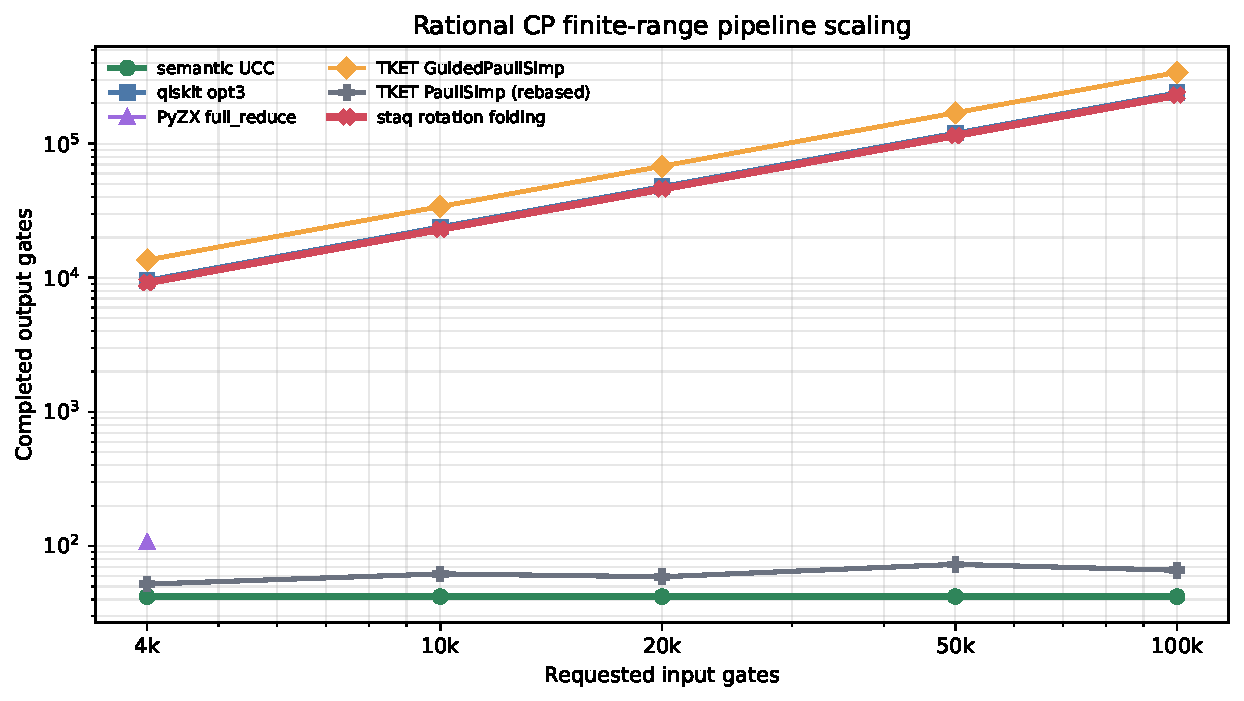
\includegraphics[width=0.95\linewidth]{figures/fourier_separation.pdf}
\caption{Fixed-width non-inverse Fourier-layer scaling on the rational
$H D^r H$ witness. Semantic UCC remains at 42 gates and rebased TKET
PauliSimp returns 52--73 gates across the five scales. Public staq
rotation folding, \texttt{qiskit opt3}, and TKET GuidedPauliSimp grow
with input size; PyZX \texttt{full\_reduce} completes at 4k and reaches
the time budget at larger scales. Status-only cells are omitted from
numerical curves.}
\label{fig:fourier-separation}
\end{figure}

\begin{figure}[tbp]
\centering
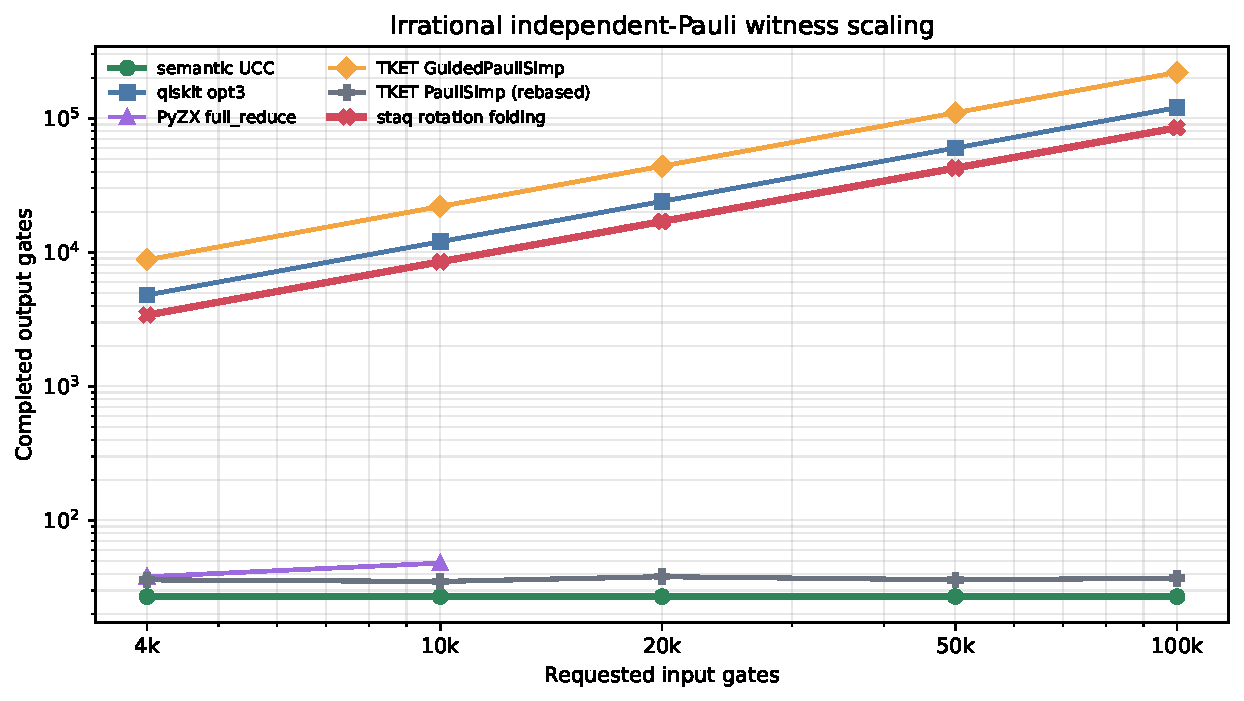
\includegraphics[width=0.95\linewidth]{figures/unbounded_witness_scaling.pdf}
\caption{Configured-pipeline scaling on the irrational independent-Pauli
witness. Semantic UCC remains at 27 gates. Rebased TKET PauliSimp
returns a small validated form at all five scales, demonstrating that a
generic pipeline can cross the formal boundary by reconstructing an
aggregate Pauli representation. Public staq rotation folding,
\texttt{qiskit opt3}, and TKET GuidedPauliSimp grow with input size.
PyZX \texttt{full\_reduce} completes at 4k and 10k, fails the numerical
tolerance at 20k, and reaches the time budget at larger scales.
Status-only cells are omitted from numerical curves.}
\label{fig:unbounded-witness-scaling}
\end{figure}

These measurements exercise the constructive side of
\cref{cor:exact-semantics-corollary} and disclose the behavior of
configured tools; they do not prove the resource bound for any real
compiler. The rebased PauliSimp result is the classification's positive
prediction in action: once a generic pass sequence reconstructs a compact
Pauli representation, the output need not grow with the flat input.
Conversely, staq's growing output and PyZX's status outcomes are not
impossibility results---they are diagnostics of configured-pipeline
behavior on this specific witness family.

\subsection{Mechanism Ablation}

\begin{table*}[tbp]
\centering
\small
\setlength{\tabcolsep}{4pt}
\begin{tabularx}{\textwidth}{@{}r *{4}{>{\raggedright\arraybackslash}X}@{}}
\toprule
Requested & semantic UCC & artifact UCC (Fourier disabled) & \texttt{qiskit} opt3 & phase-poly ref \\
\midrule
4{,}000 & 42 / 2.9 s & 9{,}588 / 18.2 s & 9{,}588 / 1.0 s & 42 / 0.2 s \\
10{,}000 & 42 / 8.7 s & 23{,}988 / 94.2 s & 23{,}988 / 5.1 s & 42 / 0.3 s \\
20{,}000 & 42 / 28.5 s & 47{,}988 / 339.3 s & 47{,}988 / 19.5 s & 42 / 0.3 s \\
50{,}000 & 42 / 20.7 s & timeout & 119{,}988 / 120.9 s & 42 / 0.5 s \\
100{,}000 & 42 / 28.7 s & timeout & 239{,}988 / 485.8 s & 42 / 0.8 s \\
\bottomrule
\end{tabularx}
\caption{Fourier-layer semantic-path ablation on the fixed-width
$H D^r H$ witness under the 600\,s budget. Disabling the Fourier-layer
IR completes at 4k--20k but materializes large outputs; 50k--100k exceed
the budget. Fourier-enabled semantic UCC and the phase-polynomial
reference return 42 gates at all sizes.}
\label{tab:fourier-ablation}
\end{table*}

\begin{figure}[tbp]
\centering
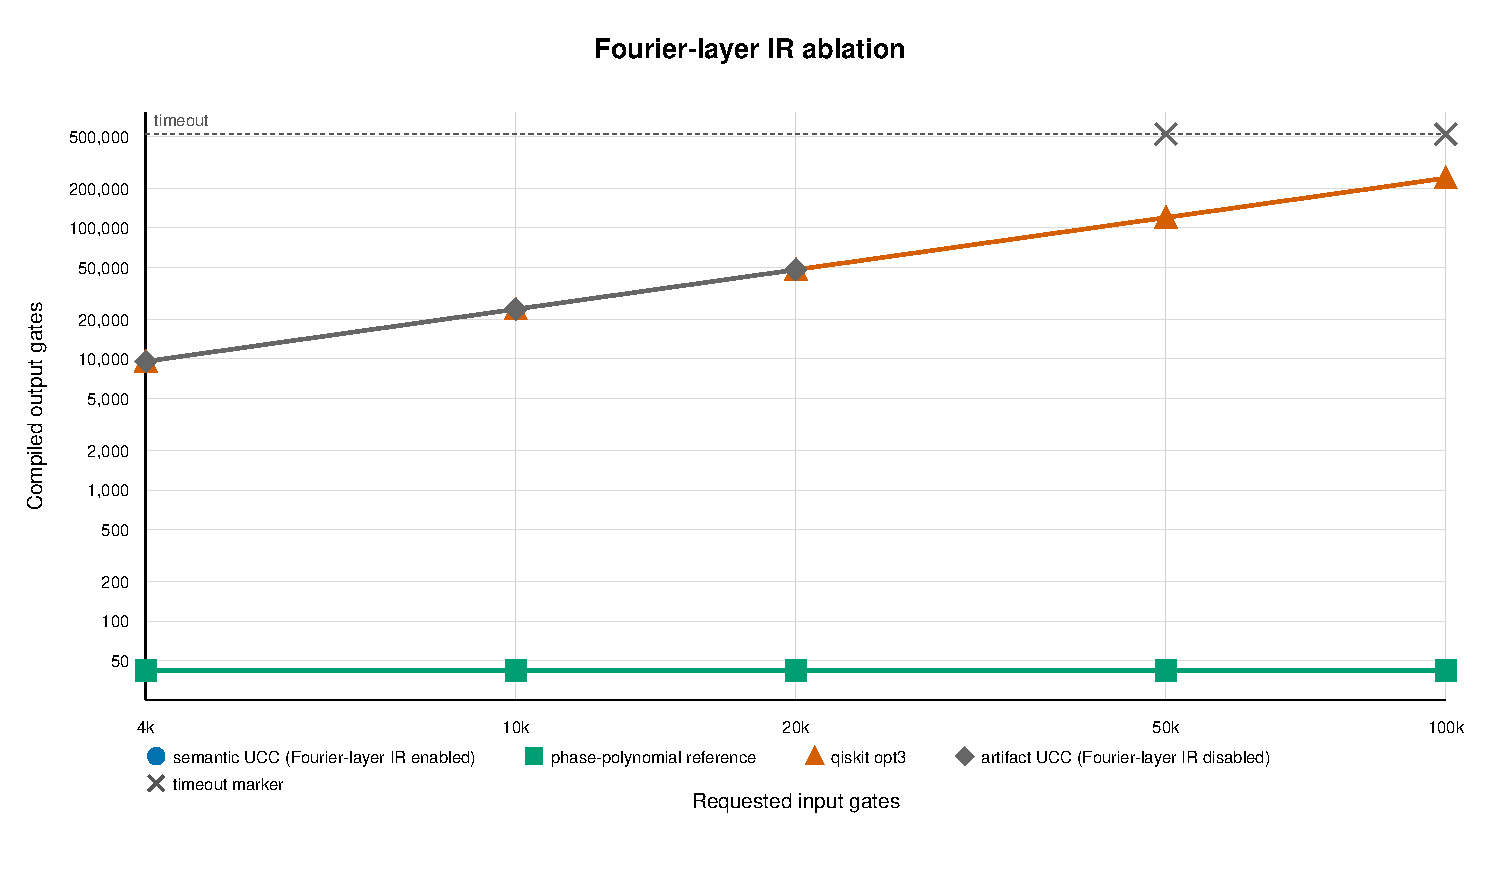
\includegraphics[width=0.95\linewidth]{figures/fourier_ablation.pdf}
\caption{Mechanism ablation for the fixed-width $H D^r H$ witness.
Disabling the Fourier-layer semantic path yields completed but linearly
large outputs through 20k and timeout rows at 50k and 100k, while
Fourier-enabled semantic UCC and the phase-polynomial reference recover
the canonical 42-gate circuit.}
\label{fig:fourier-ablation}
\end{figure}

The ablation strengthens the mechanism interpretation. With Fourier-layer
IR disabled, the compiler completes at 4k, 10k, and 20k but materializes
the same large non-aggregated outputs as \texttt{qiskit opt3}; at 50k
and 100k the disabled-IR rows exceed the 600\,s budget
(\cref{fig:fourier-ablation}). In contrast, the Fourier-enabled semantic
UCC path and the phase-polynomial reference recover the same 42-gate
canonical circuit at every tested size. Thus the constant form is tied
to semantic Fourier-layer lifting and coefficient aggregation, not
merely to a favorable ordering of flat post-lowering passes.

\subsection{Fixed-Total-Error End-to-End Synthesis and QRE}

\begin{table*}[t]
\centering
\scriptsize
\resizebox{\textwidth}{!}{%
\begin{tabular}{l r r r r r r r r r}
\toprule
pipeline & $N_{\rm rot}$ & $T$ & $d$ & physical qubits & factory qubits & factories & cycles & runtime (s) & qubit-s \\
\midrule
external TKET semantic & 29 & 798 & 23 & 258{,}152 & 253{,}920 & 16 & 13{,}317 & 0.013317 & 3{,}438 \\
materialize-first Qiskit & 23{,}992 & 2{,}679{,}110 & 31 & 468{,}968 & 461{,}280 & 16 & 57{,}966{,}528 & 57.966528 & $2.718\times10^7$ \\
semantic-first UCC & 22 & 1{,}800 & 25 & 305{,}000 & 300{,}000 & 16 & 31{,}675 & 0.031675 & 9{,}661 \\
\bottomrule
\end{tabular}}
\caption{Predeclared 20k representative slice of the fixed-total-error
campaign: $\epsilon_{\rm total}=10^{-6}$, equal synthesis allocation,
conservative $p_{\rm phys}=10^{-3}$ scenario, and 16 factories.  Each compiled
output has an independent certificate, and every unique-angle staq synthesis
returns \texttt{Check flag = 1}.  Runtime is modeled quantum execution time,
not classical compilation time.}
\label{tab:resource-consequence}
\end{table*}

The new campaign scans
$\epsilon_{\mathrm{total}}\in\{10^{-3},10^{-6},10^{-9}\}$ and assigns the
same additive fractions to every pipeline:
$0.10\epsilon_{\rm total}$ for the certified algorithmic stage,
$0.45\epsilon_{\rm total}$ for rotation synthesis, and
$0.45\epsilon_{\rm total}$ for logical failure.  For equal allocation and
$N_{\rm rot}$ output rotations, it chooses
$p=\lceil\log_{10}(N_{\rm rot}/\epsilon_{\mathrm{synth}})\rceil$ and
$\epsilon_i=10^{-p}$, hence
$\sum_i\epsilon_i\leq\epsilon_{\mathrm{synth}}$.  A second measured-cost
greedy allocation spends only this decimal slack; it is an upper construction,
not an optimality claim.  Each IEEE-serialized angle is actually synthesized
by the frozen deterministic GMP build of staq \texttt{grid\_synth}.  Across
670 checked angle--precision pairs, the reported error never exceeds the
allocated radius; exact multiples of $\pi/4$ use staq's checked exact branch.

The full $2\times3\times3\times2\times2\times4=288$ matrix crosses two target
sizes, three pipelines, three total errors, two allocation policies, two QEC
profiles, and 1/4/16/32 factories.  All 288 rows are
\texttt{completed\_valid}, carry a content-addressed exact-symbolic or dense
$n\leq6$ certificate, and satisfy the requested total-error bound.  The two
surface-code profiles use $p_{\rm phys}=10^{-3}$ and $10^{-4}$, respectively,
with separately frozen data/factory coefficients, factory periods, and cycle
times.  They choose the least odd $d$ meeting the disclosed union bound.  These
are executable sensitivity scenarios rather than vendor estimates.

\begin{figure}[tbp]
\centering

\includegraphics[width=0.99\linewidth]{../../figures/qre_pareto.pdf}
\caption{Physical-qubit/runtime Pareto grid at the representative 20k,
$\epsilon_{\rm total}=10^{-6}$ slice.  Labels give factory counts.  The
external TKET path receives a materialized CX--$R_Z$--H bridge but reconstructs
a compact phase form before synthesis, so it is classified as
semantic-capable.}
\label{fig:qre-pareto}
\end{figure}

The physical point is the ordering of semantic aggregation relative to
synthesis. In a fault-tolerant pipeline, arbitrary rotations are
eventually approximated by discrete resources such as Clifford+$T$
sequences. If the compiler first materializes $r$ separate rotations
and only later synthesizes them, the resource estimator sees $r$
independent approximation tasks. A resource-rich pipeline instead
combines the coefficients first and presents one aggregated rotation per
phase term. An FT toolchain that reconstructs the phase polynomial
before synthesis collapses this multiplicity itself and should be
classified on the semantic-capable side of the comparison
(see \cref{sec:ft-consequences} for the model-specific resource discussion).


\section{Application Workloads}
\label{sec:workloads}

\subsection{Workload Specification}

The application workloads cover four categories: (1) natural commuting
workloads (Ising/MaxCut cost evolution, diagonal Hamiltonian simulation,
QFT arithmetic, QPE controlled powers, phase-polynomial blocks);
(2) non-fully-commuting controls (aggregable blocks in Trotter/Suzuki,
QAOA with no cross-mixer merging, block encoding);
(3) negative controls (random Clifford+rotation, routing-dominated
circuits); (4) the controlled packing family
(\cref{def:packing-construction}) with growing $m$, fixed $\epsilon$,
reported in \cref{sec:packing-scaling}.

\subsection{Strong Baseline Comparison}

The comparison includes Qiskit \texttt{optimization\_level=3}~\cite{javadi2024qiskit},
TKET PauliSimp (rebased)~\cite{sivarajah2021tket,cowtan2020phase}, TKET
GuidedPauliSimp, PyZX \texttt{full\_reduce}~\cite{kissinger2020pyzx}, staq
rotation folding~\cite{amy2020staq}, and PhasePoly-style
methods~\cite{nam2018automated}. Each tool reports recommended and unified
target-basis configurations. Bridge loss is measured. Status outcomes
(timeout, memory error, correctness failure, predicate error) are recorded
separately from numerical results.

The complete cross-compiler evidence is \cref{tab:matched-matrix}: TKET
PauliSimp supplies the Pauli-network/global-semantic class and PyZX
\texttt{full\_reduce} supplies the graph/global-IR class.  All 525 cells use the
same target, declared $\{\mathrm{CX},RZ,H\}$ basis, exact target error, QASM2
bridge rule, 30\,s timeout, 2\,GiB RSS cap, and common certificate policy.
The other external rows in this paper retain their own immutable campaign
manifests and are not merged across timeout, backend, or tool-version regimes.

\subsection{Real-Task Panel}

\begin{table*}[htbp]
\centering
\scriptsize
\begin{tabular}{lccccc}
\toprule
Instance & Method & Gates & Depth & CX & Runtime \\
\midrule
\multirow{4}{*}{\texttt{REAL24-phase-est.}}
  & translation only & 159{,}838 & 121{,}214 & 67{,}608 & 0.080 s \\
  & qiskit opt3 & 166{,}805 & 119{,}204 & 58{,}491 & 1.298 s \\
  & upstream UCC v0.4.12 default & 471{,}819 & 328{,}271 & 58{,}491 & 80.923 s \\
  & semantic UCC & 166{,}805 & 119{,}204 & 58{,}491 & 1.364 s \\
\midrule
\multirow{4}{*}{\texttt{REAL24-grover}}
  & translation only & 85{,}403 & 55{,}892 & 33{,}408 & 0.104 s \\
  & qiskit opt3 & 79{,}029 & 54{,}163 & 32{,}544 & 0.552 s \\
  & upstream UCC v0.4.12 default & 287{,}047 & 152{,}298 & 32{,}544 & 1.915 s \\
  & semantic UCC & 79{,}029 & 54{,}163 & 32{,}544 & 0.556 s \\
\midrule
\multirow{4}{*}{\texttt{REAL24-qaoa}}
  & translation only & 36{,}512 & 2{,}416 & 23{,}808 & 0.022 s \\
  & qiskit opt3 & 36{,}512 & 2{,}416 & 23{,}808 & 0.272 s \\
  & upstream UCC v0.4.12 default & 167{,}833 & 7{,}133 & 23{,}808 & 1.010 s \\
  & semantic UCC & 36{,}512 & 2{,}416 & 23{,}808 & 0.273 s \\
\bottomrule
\end{tabular}
\caption{Official real algorithm-family instances. The upstream UCC
v0.4.12 row is the frozen pre-semantic default defined in the provenance
map of Appendix~B. Parity with \texttt{qiskit opt3} reflects conservative
portfolio selection; this panel is an anti-regression check, not evidence
of semantic recovery.}
\label{tab:real-instances}
\end{table*}

\begin{figure}[tbp]
\centering
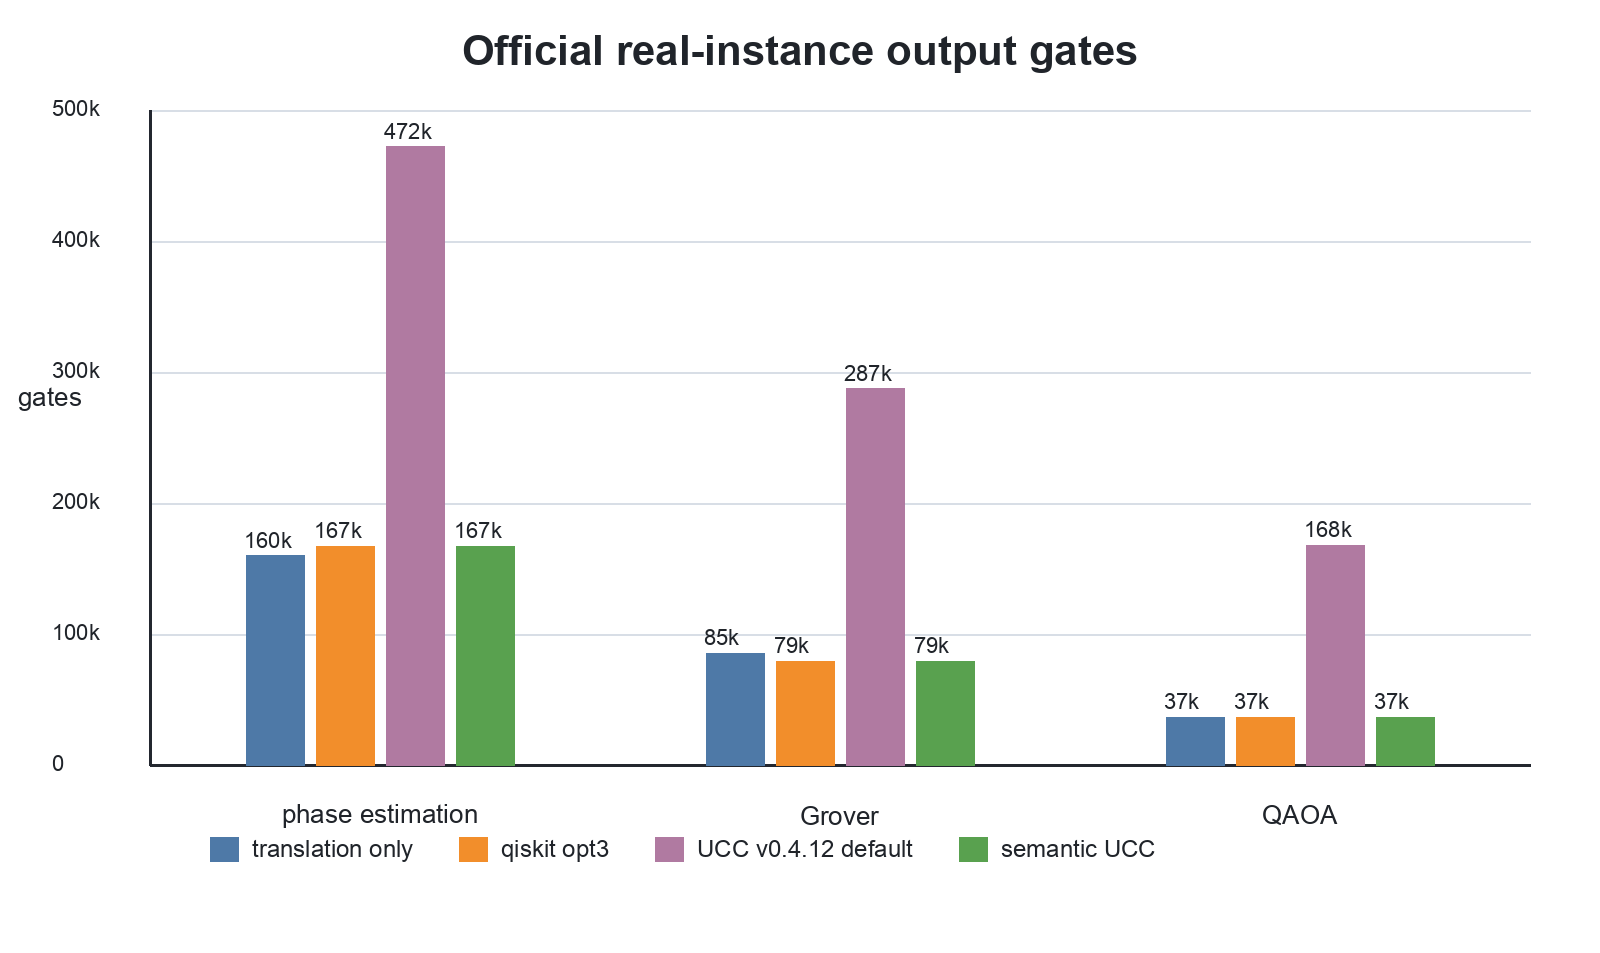
\includegraphics[width=0.95\linewidth]{figures/real_instance_grouped_bar.png}
\caption{Total output gate counts on the three official real instances.
The semantic UCC artifact matches \texttt{qiskit opt3}-level output
quality while substantially improving over the upstream UCC v0.4.12
pre-semantic default.}
\label{fig:real-instance-bars}
\end{figure}

These results support the recoverability-parity regime
(\cref{fig:real-instance-bars}): the semantic artifact matches
\texttt{qiskit opt3}-level output quality while improving over the
upstream UCC v0.4.12 pre-semantic default of \cref{tab:real-instances} by
approximately 65\%, 73\%, and 78\% gate reduction on the three instances.
The selector cost in this panel is the implementation's conservative
structural score $\kappa = \text{gates} + \text{depth} +
10\cdot\text{multi-qubit}$, with candidate-control guards; the factor
$10$ is a conservative lexicographic-style heuristic favoring lower
two-qubit exposure, used only for portfolio selection. This explains the
\texttt{REAL24-phase-est.} row (source key
\texttt{phase\_estimation\_real}) in which translation-only has fewer
total gates than the selected candidate but more \texttt{cx} gates and a
higher score ($957{,}132$ versus $870{,}919$). This quality-recovery
pattern confirms that semantic lifting behaves as an anti-regression
mechanism on workloads beyond the minimal Fourier construction.

\subsection{Natural-Kernel Factorial Ablation}
\label{sec:natural-factorial}

To separate semantic preservation from portfolio fallback, we run a full
$2^5$ factorial design over semantic lift, selector, cache, preset
optimization, and projected selection.  The seven eight-qubit kernels are
QAOA/Ising cost evolution, diagonal Hamiltonian simulation, QFT arithmetic,
QPE controlled powers, Trotterized Ising evolution, a random
Clifford--rotation negative control, and a routing-dominated negative control.
Five seeds give $7\times32\times5=1120$ cells; all complete and pass the exact
region-phase-table and boundary-sequence certificate.  Each cell also records
runtime, RSS, structured IR nodes, gates, depth, CX, cache hits/misses,
selected candidate, and all factor levels.  Historical serialized-output-bit
columns are not used because their payload files were not retained.  The
revised runner emits a codec output, certificate, serialized DAG, all five
formal components, $p$, and a verified manifest for every new cell.
Preset-on cells additionally carry a separately labelled configured-pass
contract check; that diagnostic is not promoted to theorem-domain evidence,
and the causal contrast below disables the preset entirely.

The causal contrast below disables both selector and preset, so neither a
portfolio choice nor a downstream preset compiler can create the measured
gap.  It pairs semantic-lift off/on at identical workload, seed, cache, and
projected-selection settings.  Positive kernels have strictly positive gate
and CX reductions; both negative controls record zero structural effect in
every paired cell.

\begin{table*}[tbp]
\centering
\small
\begin{tabularx}{\textwidth}{@{}l r X X@{}}
\toprule
Workload & paired cells & gate reduction, mean [95\% CI] & CX reduction, mean [95\% CI] \\
\midrule
qaoa\_ising & 20 & 216.0 [216.0,216.0] & 144.0 [144.0,144.0] \\
diagonal\_hamiltonian & 20 & 1092.0 [1092.0,1092.0] & 728.0 [728.0,728.0] \\
qft\_arithmetic & 20 & 150.0 [150.0,150.0] & 100.0 [100.0,100.0] \\
qpe\_controlled\_powers & 20 & 84.0 [84.0,84.0] & 56.0 [56.0,56.0] \\
ising\_trotter & 20 & 168.0 [168.0,168.0] & 112.0 [112.0,112.0] \\
negative\_random\_clifford & 20 & 0.0 [0.0,0.0] & 0.0 [0.0,0.0] \\
negative\_routing & 20 & 0.0 [0.0,0.0] & 0.0 [0.0,0.0]
 \\
\bottomrule
\end{tabularx}
\caption{Paired semantic-lift effect with selector and preset disabled.
Reduction is the flat output minus the semantic-lift output.  Cache and
projected-selection levels and all five seeds remain balanced.}
\label{tab:natural-factorial}
\end{table*}

\begin{figure}[tbp]
\centering
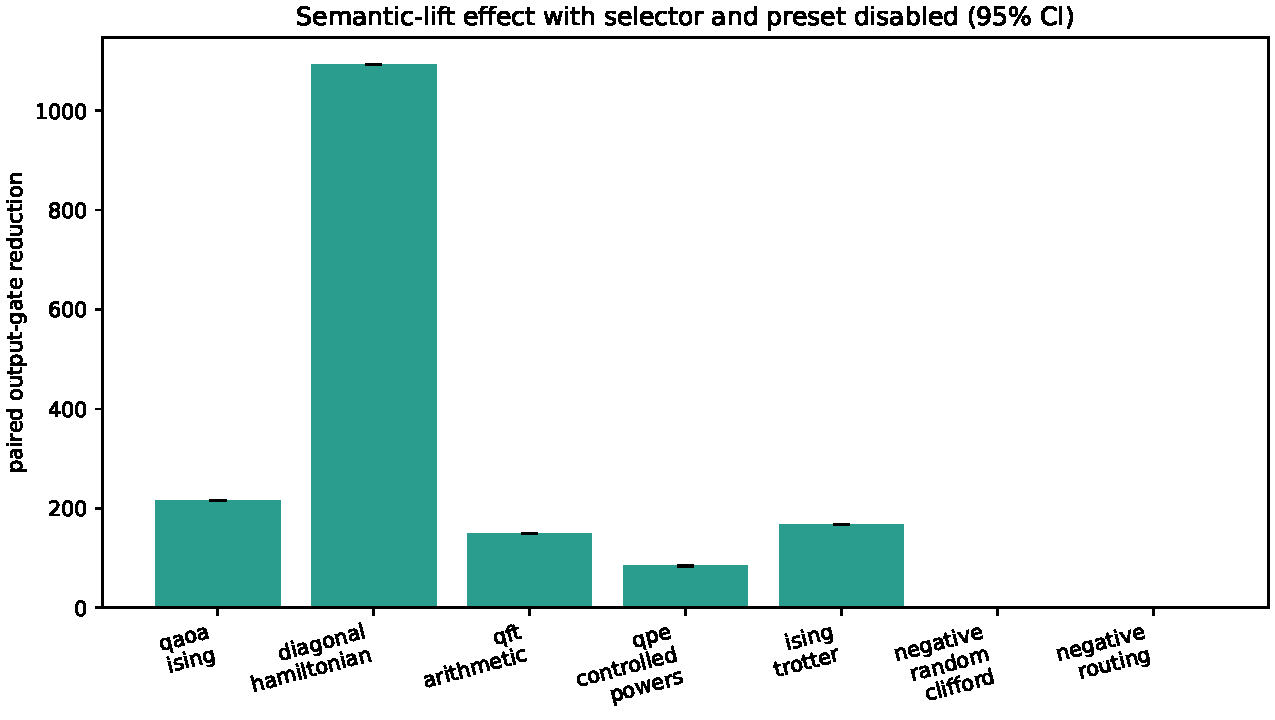
\includegraphics[width=0.98\linewidth]{research/natural_factorial/semantic_lift_selector_off.pdf}
\caption{Factorial-ablation gate effect with selector and preset disabled.
The five structured kernels benefit, while the two negative controls do not.
This is an executable mechanism test, not a claim of universal workload
advantage.}
\label{fig:natural-factorial}
\end{figure}

Together with the historical real panel, the evidence now has two distinct
roles: \cref{tab:real-instances} is an anti-regression diagnostic, whereas
\cref{tab:natural-factorial,fig:natural-factorial} isolates the semantic-lift
factor without selector or preset fallback on controlled algorithm-family
kernels.  Neither is used as an empirical proof of the streaming lower bound.


\section{Model-Specific Fault-Tolerant Resource Consequences}
\label{sec:ft-consequences}

The representation gap propagates into the fault-tolerant resources of the
explicit model in
\cref{tab:resource-consequence,fig:qre-pareto,fig:qre-sensitivity}.  Over all 96
matched target/error/allocation/QEC/factory settings, materialize-first uses
385--1{,}753 times the logical $T$ states and 538--5{,}573 times the spacetime
volume of semantic-first.  No reversal occurs within the scanned error and
factory grid.  This is not a claim that the authors' implementation dominates
other semantic tools: external TKET \texttt{PauliSimp} reconstructs the phase
structure before synthesis and uses 0.443--0.536 times the semantic-first $T$
states on this witness.  Correctly crediting that recovery is part of the
comparison.

These values are outputs of actual checked angle synthesis followed by the
disclosed scheduling models, not universal hardware predictions.  The
absolute physical numbers still depend on routing, correlated-error, factory
layout, feed-forward, and code-distance assumptions outside this campaign.
The complete sensitivity plot and all preflight anomalies are retained in the
root QRE artifact package.

\begin{figure*}[tbp]
\centering

\includegraphics[width=0.98\textwidth]{../../figures/qre_sensitivity.pdf}
\caption{Sensitivity to total error, QEC profile, and factory count on the 20k
witness.  Top: logical $T$ demand and the conservative-profile spacetime
volume.  Bottom: ratios to semantic-first, with bands spanning both QEC
profiles and all four factory counts.  The dashed line is equality.  No
materialize-first reversal occurs in the measured grid; the strong external
TKET path is reported on the semantic-capable side.}
\label{fig:qre-sensitivity}
\end{figure*}


\section{Related Work}
\label{sec:related-work}

\paragraph{Phase-polynomial, Pauli-gadget, and ZX optimization.}
Commuting-rotation aggregation is a standard optimization
target~\cite{amy2014tdepth,nam2018automated,ross2016optimal,cowtan2020phase,sivarajah2021tket,duncan2020graph,kissinger2020reducing,kissinger2020pyzx}.
Our contribution is different: we formalize a representation-dependent
recoverability boundary with an explicit
$\epsilon$--resource tradeoff, connect it to communication complexity, and
measure model-specific fault-tolerant consequences under one disclosed QRE.

\paragraph{Compiler IRs, verified compilation, and full-stack tooling.}
Quantum software stacks use intermediate representations to preserve
information across lowering~\cite{steiger2018projectq,javadi2024qiskit,sivarajah2021tket,martiel2022architecture,watkins2024surfacecode,hietala2021verified,mills2021application,fellous2023optimizing}.

\paragraph{Classical lower-bound methodology.}
The proof imports fooling-set and communication-complexity reasoning into
a quantum-compilation representation
question~\cite{sipser2012introduction,kushilevitz1997communication,alur2010streaming}.


\section{Discussion}
\label{sec:discussion}

\subsection{Representation as a Resource}

The central message is that representation is a computational resource in
quantum compilation. A compiler receiving a semantic representation
preserving generator--coefficient structure can aggregate in $O(m)$
records.  The cyclic packing gives
$\Omega(m\log(1/\epsilon))$ bits separately for family-relative and
self-contained output codes and is compatible with an $r$-round modular
share stream.  In the stated forward-scan model its pass-explicit frontier is
$\overline A_p+(2p-1)S\geq
(1-\delta)m\log_2K-h_2(\delta)$
(\cref{thm:w1-unified-frontier}).  Thus a deferred flat compiler needs
$S=\Omega(m\log K/p)$.  The block hybrid attains
$S=O((m/p)\log(K+1))$ with compact family-relative output, within the
proved constant factor, while the direct semantic vector uses only
$O(\log(mK))$ state
(\cref{prop:w1-block-hybrid,prop:w1-semantic-upper}).  The older binary
two-round theorem remains a sharper zero-error, one-pass special case.

This boundary is channel-explicit.  Equation~\eqref{eq:info-budget}
serializes control, store, window structure, every live parameter, every
live IR object, cache/hash layout, dynamic-pass state, and random seed.  A
compiler that reconstructs a global aggregate---as
rebased TKET PauliSimp does on the fixed-width witnesses---may succeed, but
its reconstruction table or graph is charged in $B_{\mathrm{cut}}$ rather
than treated as a free semantic side channel.

\subsection{Scope and Limitations}

\begin{enumerate}[leftmargin=1.5em]
    \item The results have different scopes.  The unified theorem
    (\cref{thm:w1-unified-frontier}) covers $r$-round additive shares,
    randomized failure, and $p=p(m)$ forward scans of the round-major
    stream, but charges all $2p-1$ serialized crossings and claims only a
    constant-factor state upper envelope.  Reverse scans, an uncharged
    random-access input oracle, or a different output code are outside that
    theorem.  The older representation-dependent tradeoff
    (\cref{thm:main-tradeoff}) is scoped to the two-round masked-share
    stream and gives the stronger deterministic one-pass mask count.  The
    exact-semantics corollary is scoped to fixed width, constant pass/cut
    budget, and certified noncollision.  The growing-width theorems instead
    use the complete bit codec and allow random access and dynamic
    $p=p(m,I,\rho)$.  The decoder is representation-invariant, but all
    syntax lengths retain their declared encoding semantics.
    \item The tuned cyclic packing is stated for
    $0<\epsilon\leq1/8$ and chooses sharing modulus
    $Q_\epsilon=K_\epsilon+1$.  Its coefficient interval can cross $\pi$;
    \cref{thm:w1-exact-separation} handles circular distance and global
    phase exactly.  The prior no-wrap packing and the binary/$\mathbb Z_3$
    theorem remain separate valid specializations.
    The configured scaling experiment uses $K=2$, $\Delta=\pi/4$ and is not
    claimed to instantiate the masked-share theorem.
    \item The fixed-total-error experiment performs actual Clifford+$T$
    synthesis and executable surface-code calculations under two disclosed
    physical/QEC profiles, but these profiles share one phenomenological model
    family.  Absolute physical counts still require cross-validation under an
    independent estimator and architecture-specific routing/factory layouts.
    \item The packing-family scaling experiment
    (\cref{sec:packing-scaling}) links the growing-$m$ theorems to
    configured-pipeline behavior.  The instrumented reference compilers now
    measure the masked-share cut fields directly
    (\cref{sec:cut-tracing}); broader natural-workload tracing and independent
    QRE cross-validation remain follow-up work.
\end{enumerate}


\section{Conclusion}
\label{sec:conclusion}

We have formalized approximate recoverability with a growing-width token
codec and a bit-level cut budget whose five executable serialization fields
include parameter, RAM/cache, random-seed, dynamic-pass, and IR channels.
The cyclic $K_\epsilon$-ary family has exact minimum separation
$2\sin(\pi/(2(K_\epsilon+1)))$, satisfies
$K_\epsilon=\Theta(1/\epsilon)$, and admits semantic and $r$-round flat
representations of the same $U_x$ even though no individual update
determines $x_j$.  For randomized failure $\delta$ and $p=p(m)$ forward
passes, each named output code and the prefix-side commitment plus crossing
transcript require at least
$(1-\delta)m\log_2K_\epsilon-h_2(\delta)$ expected bits.  Hence a deferred
compiler satisfies $(2p-1)S\geq
(1-\delta)m\log_2K_\epsilon-h_2(\delta)$.  A block hybrid reaches compact
family-relative output with
$S=O((m/p)\log(K_\epsilon+1))$, within the proved constant factor, and the
randomized relative-output bound is matched up to framing.  The semantic
vector achieves compact output with logarithmic state.  The exact-semantics
corollary retains the fixed-width final-output lower bounds of the prior
version. Controlled validation confirms the constructive side.  Under the
evidence separation of \cref{tab:evidence-classes}, the checked three-cut
fixture validates accounting but is not lower-bound evidence; a compliant
rerun of the restart tracer is required to retest the formal commitment--cut
tradeoff.  The matched matrix, packing counts, and workload ablations remain
configured-pipeline diagnostics.  Fixed-total-error synthesis/QRE exposes a
downstream physical consequence under an explicit model. Recoverability should
be treated as a controlled variable in compilation and resource estimation.


\section*{Reproducibility}
\label{sec:reproducibility}

The frozen research directory includes a standardized artifact entry
point, environment snapshot, output manifest, and reproducibility guide.
The rational-witness period certificate, exact-integer output, and hashes
are in \path{research/rational_witness/}.  The exact certificate specification,
symbolic checker, and mutation/dense audit are in \path{certificates/} and
\path{data/frozen/certificate_audit.json}; the historical event-level cut
trace, historical fixed-budget synthesis/QRE, and keyed table registry are in
\path{research/cut_trace/},
\path{research/fixed_budget_qre/}, and
\path{research/experiment_registry/}, respectively.  The complete matched
matrix, multifactor summaries, natural-kernel factorial ablation, immutable
campaign hierarchy, and claim--evidence matrix are in
\path{research/matched_representation/},
\path{research/natural_factorial/},
\path{research/campaign_manifests/}, and
\path{research/claim_evidence/}.  The version-one codec, file-backed
accountant, and checked deterministic trace are in \path{encoding/},
\path{instrumentation/}, and \path{instrumentation/example_trace/}; the
historical cut-trace and matched bit summaries are not accepted by the new
manifest verifier without a campaign rerun.  The W7 fixed-total-error schemas,
two QEC profiles, factory grid, measured 288-row Parquet table, freeze manifest,
analysis, raw angle records, and publication figures are in \path{qre/},
\path{data/frozen/qre_results.parquet},
\path{data/runs/w7-fixed-total-error-20260803-local/}, and \path{figures/};
\path{QRE_REPORT.md} records the limitations and both retained preflight
failures.


\appendix
\counterwithout{equation}{section}
\section{Supplementary Theory and Full Proofs}

\subsection{Operational Gap Notation}

For reference, the experimental gap can be written without adding another
formal theorem hypothesis. Let:
\begin{itemize}[leftmargin=1.5em]
    \item $L_B(C)$ be exact lowering into target basis $B$,
    \item $\kappa$ be a conservative structural cost,
    \item $\mathcal{T}_K(C)$ be the bounded set of semantic candidates produced
    by the semantic lift under budget $K$,
    \item $\mathfrak{A}$ be a configured post-lowering pipeline family used for
    an experiment.
\end{itemize}

Define the $(K,w)$-representation gap of $C$ by
\[
\mathrm{Gap}^{K,w}_{\mathrm{rep}}(C)
:=
\inf_{A \in \mathfrak{A}} \kappa(A(L_B(C)))
-
\inf_{T \in \mathcal{T}_K(C)} \kappa(L_B(T)).
\]
Define the operational recoverability gap by
\[
\mathrm{Gap}^{K,w}_{\mathrm{rec}}(C)
:=
\kappa(C_{\mathrm{flat}}^\star) - \kappa(C_{\mathrm{term}}^\star),
\]
where $C_{\mathrm{flat}}^\star$ is the best candidate recovered from the flat
basis-lowered representation and $C_{\mathrm{term}}^\star$ is the best
candidate recovered from the bounded semantic term representation.

The meaning is simple: semantics may survive lowering, while cheap
recoverability of the opportunity may not. This notation is operational and
experimental; the formal lower bound in the main text is the budget-explicit
final-output theorem for finite-window transducers.

\begin{definition}[Aggregate recovery]
\label{def:aggregation-equivalent-recovery}
Consider the Fourier-layer family
$C_{m,r}=H_{\Lambda}D_m(\boldsymbol{\theta})^rH_{\Lambda}$ with
$D_m(\boldsymbol{\theta})=\prod_{j=1}^m e^{-i\theta_jP_j/2}$. A compiler
performs \emph{aggregation-equivalent recovery} on this family if, for each
non-removable term $P_j$, its successful output can be associated with an
$O(1)$-size record, subcircuit, or algebraic object whose coefficient is
equivalent modulo $2\pi$ to the aggregate $r\theta_j$. The object may be
explicit, as in a phase-polynomial or commuting-diagonal IR, or implicit, as
in a specialized rewrite, lookup, ZX transformation, or synthesis routine that
computes the same aggregate diagonal action without storing all $r$ lowered
occurrences separately.
\end{definition}

\begin{proposition}[Operational recovery channels]
\label{prop:classification-boundary}
For the Fourier-layer family, a pipeline that recovers the constant
fixed-width output can be classified by the channel through which it carries
the aggregate coefficient information. Examples include:
\begin{enumerate}[leftmargin=1.5em]
    \item store enough persistent summary information to carry the aggregate;
    \item lift enough lowered volume into a richer IR to reconstruct the
    aggregate;
    \item use nonlocal provenance information from before basis lowering that
    already contains the aggregate;
    \item reconstruct a global semantic representation equivalent to a
    phase-polynomial, ZX, stabilizer-phase, or commuting-diagonal Hamiltonian
    object.
\end{enumerate}
Consequently, a successful future flat-looking implementation would not by
itself refute the main theorem. It would instead classify the implementation by
identifying where the aggregate information crosses the finite-state boundary,
or by showing that the formal transducer model is missing a cheaper channel.
\end{proposition}

\begin{proof}[Justification]
The fixed-width theorem lower-bounds final output length for constant-budget
finite-window transducers on a certified noncolliding family. A pipeline that
achieves the semantic constant output must still represent the aggregate
coefficients that distinguish the noncolliding cases. The listed channels are
implementation-level ways to carry that information. This is a classification
statement rather than an optimality claim.
\end{proof}

\subsection*{Additional Structural Families}

The artifact also targets phase-ladder, mirrored, and conjugation patterns that
appear in QPE/QFT-style workloads and Grover-style workloads. These families
are not used here as additional theorem instances. They are best read as
structural stress families: the semantic controller preserves repeated
phase-heavy ladders, mirrored shells, and conjugation shells long enough to
compare projected costs before materializing the selected candidate.

For phase-ladder workloads, the relevant empirical question is whether bounded
semantic terms preserve a repeated commuting-diagonal opportunity that is
harder to recover after early lowering. For mirrored and conjugation workloads,
the relevant empirical question is whether the artifact recognizes repeated
shell structure and avoids materializing every candidate before selection. The
Grover and mirrored-shell experiments in Appendix~C are therefore empirical
positive cases and robustness checks, not support for a separate theorem-level
family separation.

\subsection{Self-Contained Rational CP Period Certificate}
\label{app:sec:rational-period}

The canonical four-qubit rational witness has diagonal block
\begin{equation*}
\begin{aligned}
D={}&\prod_{j=0}^{3}RZ_j(\theta_j)
 \prod_{0\leq a<b\leq3}CP_{ab}(\theta_{ab}),\\
\boldsymbol\theta_{RZ}/\pi
={}&(1/7,1/8,1/9,1/10),\\
(\theta_{01},\theta_{02},\theta_{03})/\pi
={}&(1/12,1/13,1/14),\\
(\theta_{12},\theta_{13},\theta_{23})/\pi
={}&(1/14,1/15,1/16).
\end{aligned}
\end{equation*}
For a reduced rational angle $\theta/\pi=p/q$, both $RZ(\theta)$ and
$CP(\theta)$ have projective single-term order
\begin{equation*}
 \operatorname{ord}(p/q)
 =\frac{2q}{\gcd(|p|,2q)},
\end{equation*}
because the relevant relative phase is $p/q$ modulo $2$.  The complete
single-term certificate is
\begin{center}
\begin{tabular}{lccc}
\toprule
term & support & $\theta/\pi$ & $T_j$\\
\midrule
$RZ_0$ & $0$ & $1/7$ & $14$\\
$RZ_1$ & $1$ & $1/8$ & $16$\\
$RZ_2$ & $2$ & $1/9$ & $18$\\
$RZ_3$ & $3$ & $1/10$ & $20$\\
$CP_{01}$ & $01$ & $1/12$ & $24$\\
$CP_{02}$ & $02$ & $1/13$ & $26$\\
$CP_{03}$ & $03$ & $1/14$ & $28$\\
$CP_{12}$ & $12$ & $1/14$ & $28$\\
$CP_{13}$ & $13$ & $1/15$ & $30$\\
$CP_{23}$ & $23$ & $1/16$ & $32$\\
\bottomrule
\end{tabular}
\end{center}
Hence
\begin{equation*}
\begin{aligned}
T_{\mathrm{terms}}
&=\operatorname{lcm}(14,16,18,20,24,26,28,28,30,32)\\
&=2^5\cdot3^2\cdot5\cdot7\cdot13=131040,
\end{aligned}
\end{equation*}
which proves that $D^{131040}$ is a global phase.  To certify minimality
for the product rather than merely obtain this common upper bound, subtract
the phase of $0000$.  For $z=z_0z_1z_2z_3$, the exact relative phase is
\begin{equation*}
\begin{aligned}
w(z)={}&z_0/7+z_1/8+z_2/9+z_3/10\\
 &+z_0z_1/12+z_0z_2/13+z_0z_3/14\\
 &+z_1z_2/14+z_1z_3/15+z_2z_3/16
 \pmod 2.
\end{aligned}
\end{equation*}
In particular,
\begin{equation*}
\begin{aligned}
 w(1011)&=\frac{37007}{65520},\\
 \operatorname{ord}(w(1011))
 &=\frac{2\cdot65520}{\gcd(37007,2\cdot65520)}\\
 &=131040.
\end{aligned}
\end{equation*}
Thus no smaller positive power of $D$ is a global phase, and
$T=131040$ exactly.  It follows that
$D^1,\ldots,D^R$ are pairwise distinct up to global phase for every
$R<T$.

The machine certificate uses only Python \texttt{fractions.Fraction} and
prints all 16 relative numerators, denominators, and orders.  The frozen
integer output contains
\begin{equation*}
\begin{gathered}
\texttt{term\_order\_lcm=131040},\\
\texttt{relative\_order\_lcm=131040},\\
\texttt{minimality\_state\_1011\_order=131040},\\
\texttt{exact\_global\_phase\_period\_T=131040}.
\end{gathered}
\end{equation*}
The reproducibility files and hashes are listed below; each digest is split
at its 32-hex midpoint only for typesetting.
\begin{itemize}[leftmargin=1.5em]
 \item verifier: \path{research/rational_witness/verify_period.py},
 SHA256 \texttt{c7c90f26e00e515383e94e4bbd707574}\allowbreak
 \texttt{eb3aabf94ad71c3cd5e2cdb8d5db7e76};
 \item integer output:
 \path{research/rational_witness/period_certificate.txt}, SHA256
 \texttt{375295d776f21ea2a82ee4f2bab5205d}\allowbreak
 \texttt{25bfef85ee864900baacfbd80be9bd6e};
 \item manifest: \path{research/rational_witness/SHA256SUMS}.
\end{itemize}
From the repaired-manuscript root, the byte-for-byte check is
\begin{quote}
\footnotesize
\texttt{cd research/rational\_witness}\\
\texttt{python3 verify\_period.py \textbackslash}\\
\texttt{\quad --check period\_certificate.txt}
\end{quote}

\subsection{Full Proofs for the Transducer Lower Bound}
\label{app:sec:full-proofs}

This section supplies the full finite-state proof layer underlying
\Cref{thm:final-output,cor:finite-tail,cor:counting-toll}. The main text states
the shorter version; the appendix keeps the pumpability data explicit.
The following statements restate the main-text theorem and corollaries with
full hypotheses and complete proofs; they are not additional independent
results.

\subsubsection{Pumpable Pair Families}

Persistent store can depend on $r$, so the induction tracks both a store value
and a tape word. In this subsection, $D$ in pumpability data denotes a period
modulus, not the diagonal witness layer in $C_r=H_\Lambda D^rH_\Lambda^{-1}$.
The next definition restates the main-text pumpable-pair definition with
explicit residue data for the full proof.

\begin{definition}[Pumpable pair family, restated with explicit residue data]
\label{app:def:pumpable}
Let $\Gamma$ be a finite alphabet and $P$ a finite set of store values. A family
\[
  X(r)=(\beta(r),W(r))\in P\times\Gamma^*,\qquad r\in\mathbb{N},
\]
is \emph{pumpable} if there exist integers $h\ge0$ and $D\ge1$ such that for
every residue $\rho\in\{0,\ldots,D-1\}$ there are
\[
  \beta_\rho\in P,
  \qquad
  A_\rho,B_\rho,C_\rho\in\Gamma^*,
\]
with
\[
  X(h+\rho+kD)=(\beta_\rho,A_\rho B_\rho^k C_\rho)
\]
for every $k\ge0$. The word $B_\rho$ is the pump word on residue $\rho$. The
residue is \emph{live} if $B_\rho\ne\epsilon$ and \emph{collapsed} if
$B_\rho=\epsilon$.
\end{definition}

\begin{lemma}[Input pumpability]
\label{app:lem:input-pumpable}
For the fixed-width witness $T_0(r)=\Pi M^r\Sigma$, the pair family consisting
of the initial persistent store and $T_0(r)$ is pumpable with $h=0$, $D=1$,
pump word $M$, and fixed store value.
\end{lemma}

\begin{proof}
Take $A_0=\Pi$, $B_0=M$, and $C_0=\Sigma$.
\end{proof}

\subsubsection{One-Pass Propagation}

Fix a precision bound $q$ and a charged alphabet $\Gamma=\Gamma_B(q)$. Under
this bound, a pass of $\mathcal{A}$ can be viewed as an ordinary deterministic
subsequential transducer over a finite alphabet. Its finite state consists of
the ephemeral state, the persistent store, and the $w$-token window. The
end-of-pass persistent store is one component of the final finite state.

\begin{lemma}[One-pass pumpability propagation]
\label{app:lem:one-pass-pump}
Let $X(r)=(\beta(r),W(r))$ be a pumpable pair family over a finite input
alphabet. Let $\tau$ be one deterministic finite-window, finite-burst pass whose
output alphabet and store set are finite. Let
\[
  \tau(\beta(r),W(r))=(\beta'(r),W'(r))
\]
be the resulting final store and output tape. Then
$X'(r)=(\beta'(r),W'(r))$ is pumpable.
\end{lemma}

\begin{proof}
Fix pumpability data
$h,D,\{\beta_\rho,A_\rho,B_\rho,C_\rho\}_\rho$ for $X$. We first treat one
residue $\rho$, then recombine all residues into $r$-indexed pumpability data
for $X'$.

For a fixed residue $\rho$, write
\[
  W_k=A B^k C,
  \qquad
  \beta_k=\beta,
\]
where $k\ge0$ and $A,B,C,\beta$ abbreviate the residue data. Absorb the
ephemeral state, persistent store, and window into the pass's finite state set
$S$. Starting from the state determined by $\beta$, process $A$. This emits a
fixed word $O_A$ and reaches a state $s_A\in S$.

Let $f:S\to S$ be the state map obtained by reading the block $B$, and let
$o(s)\in(\Gamma')^*$ be the output emitted while reading $B$ starting in state
$s$. The sequence
\[
  s_A,\ f(s_A),\ f^2(s_A),\ldots
\]
in the finite set $S$ is ultimately periodic. Thus there exist $u\ge0$ and
$\ell\ge1$ with $u+\ell\le |S|+1$ such that
\[
  f^{t+\ell}(s_A)=f^t(s_A)
  \qquad\text{for all }t\ge u.
\]
For $k=u+v\ell+\eta$ with $0\le\eta<\ell$, the output while reading $B^k$ is
\[
\begin{aligned}
  &\bigl(o(s_A)o(f(s_A))\cdots o(f^{u-1}(s_A))\bigr)\\
  &\quad\cdot\Bigl(o(f^u(s_A))\cdots
  o(f^{u+\ell-1}(s_A))\Bigr)^v\\
  &\quad\cdot\bigl(o(f^u(s_A))\cdots
  o(f^{u+\eta-1}(s_A))\bigr).
\end{aligned}
\]
After this, the pass reads the fixed suffix $C$, emits a word depending only
on the state $f^{u+\eta}(s_A)$, and ends in a persistent store value depending
only on the same state.

Restore the residue subscripts. For each original residue
$\rho\in\{0,\ldots,D-1\}$, let $u_\rho\ge0$ and $\ell_\rho\ge1$ be the
preperiod and cycle length obtained above, let $f_\rho$, $s_{A_\rho}$, and
$O_{A_\rho}$ be the corresponding state map, post-prefix state, and prefix
output. For $0\le\eta<\ell_\rho$, let $F_{\rho,\eta}$ be the complete word
emitted while reading the fixed suffix $C_\rho$ from state
$f_\rho^{u_\rho+\eta}(s_{A_\rho})$, including the end-of-tape finalizer output,
and define
\begin{align*}
  P_\rho &:=
  o\bigl(s_{A_\rho}\bigr)o\bigl(f_\rho(s_{A_\rho})\bigr)\cdots
  o\bigl(f_\rho^{u_\rho-1}(s_{A_\rho})\bigr),\\
  Q_\rho &:=
  o\bigl(f_\rho^{u_\rho}(s_{A_\rho})\bigr)\cdots
  o\bigl(f_\rho^{u_\rho+\ell_\rho-1}(s_{A_\rho})\bigr),\\
  R_{\rho,\eta} &:=
  o\bigl(f_\rho^{u_\rho}(s_{A_\rho})\bigr)\cdots
  o\bigl(f_\rho^{u_\rho+\eta-1}(s_{A_\rho})\bigr)\cdot F_{\rho,\eta}.
\end{align*}
Let $\beta'_{\rho,\eta}$ be the end-of-pass persistent store value reached from
that state. Define
\[
\begin{aligned}
  u^*&:=\max_{\rho} u_\rho,
  &\ell^*&:=\lcmop_{\rho}\ell_\rho,\\
  h'&:=h+D u^*,
  &D'&:=D\ell^*.
\end{aligned}
\]
Each new residue $\rho'\in\{0,\ldots,D'-1\}$ decomposes uniquely as
\[
  \rho'=\rho+D\tilde\eta,
  \qquad
  \rho\in\{0,\ldots,D-1\},\quad
  \tilde\eta\in\{0,\ldots,\ell^*-1\}.
\]
For $r=h'+\rho'+k'D'$ with $k'\ge0$, the old representation
$r=h+\rho+kD$ has
\[
  k=u^*+\tilde\eta+k'\ell^*.
\]
Since $u^*\ge u_\rho$, we have $k\ge u_\rho$ for every $k'\ge0$; and since
$\ell_\rho\mid\ell^*$, the residue of $k-u_\rho$ modulo $\ell_\rho$ does not
depend on $k'$. Set
\[
  \eta:=(u^*+\tilde\eta-u_\rho)\bmod \ell_\rho,
  \qquad
  v_0:=\Bigl\lfloor\frac{u^*+\tilde\eta-u_\rho}{\ell_\rho}\Bigr\rfloor\ge0,
\]
so that
\[
  k=u_\rho+(v_0+k'\ell^*/\ell_\rho)\ell_\rho+\eta.
\]
By the output decomposition above, for every $k'\ge0$,
\[
  X'(h'+\rho'+k'D')
  =\bigl(\beta'_{\rho,\eta},\ A'_{\rho'}(B'_{\rho'})^{k'}C'_{\rho'}\bigr),
\]
where
\[
  A'_{\rho'}:=O_{A_\rho}P_\rho Q_\rho^{v_0},
  \qquad
  B'_{\rho'}:=Q_\rho^{\ell^*/\ell_\rho},
  \qquad
  C'_{\rho'}:=R_{\rho,\eta}.
\]
This is exactly pumpability of $X'$ with data $(h',D')$ and residue data
$\{\beta'_{\rho,\eta},A'_{\rho'},B'_{\rho'},C'_{\rho'}\}_{\rho'}$.
\end{proof}

\begin{corollary}[Per-tape induction, for proof]
\label{app:cor:per-tape}
Assume $\mathcal{A}$ has constant budget, so all executions use one finite
alphabet $\Gamma_B(q_*)$. For every pass index $i=0,1,\ldots,p$, the pair
family consisting of the persistent store after pass $i$ and the tape $T_i(r)$
is pumpable.
\end{corollary}

\begin{proof}
The base case is \Cref{app:lem:input-pumpable}. Apply
\Cref{app:lem:one-pass-pump} successively to passes $1,\ldots,p$.
\end{proof}

\begin{remark}[Unary scratch tapes]
\label{app:rem:unary}
If pass 1 writes one marker per input period, then
$T_1(r)=\mathtt{marker}^r$ is pumpable with live pump word
$\mathtt{marker}$. \Cref{app:lem:one-pass-pump} applies to every later
pass. A later constant-budget pass may output one marker every $c$ input
markers, permute markers, or add a fixed periodic decoration, but it remains
pumpable. It cannot turn $\mathtt{marker}^r$ into a family of $O(1)$ many
correct aggregate circuits for all noncolliding $r$; if the final pump
collapses, the final output repeats on a residue class.
\end{remark}

\subsubsection{Collapse Versus Final-Output Length}

\begin{lemma}[Pumpable outputs are bounded-or-linear on each residue]
\label{app:lem:bounded-or-linear}
Let $W(r)$ be a pumpable word family with data
$(h,D,A_\rho,B_\rho,C_\rho)$. For $r=h+\rho+kD$:
\begin{enumerate}[label=(\alph*)]
\item if $B_\rho=\epsilon$, then $W(h+\rho+kD)$ is independent of $k$;
\item if $B_\rho\ne\epsilon$, then
\[
  |W(h+\rho+kD)|\ge k.
\]
\end{enumerate}
Consequently, on a live residue,
\[
  |W(r)|\ge \frac{r-h-D+1}{D}
\]
for all $r\ge h+D$ in that residue.
\end{lemma}

\begin{proof}
Both statements are immediate from
$W(h+\rho+kD)=A_\rho B_\rho^k C_\rho$. If $B_\rho\ne\epsilon$, then
$|B_\rho|\ge1$, so $|A_\rho B_\rho^k C_\rho|\ge k$. Since
$r=h+\rho+kD$ and $0\le\rho<D$, $k\ge(r-h-D+1)/D$.
\end{proof}

\begin{lemma}[Correct noncolliding final outputs cannot collapse]
\label{app:lem:no-collapse}
Assume finite-range noncollision (Assumption~\ref{ass:noncollision}) with
$N(R)=R$ on the interval $1\le r\le R$. Suppose the final output family
$T_p(r)$ is pumpable with data $(h,D,A_\rho,B_\rho,C_\rho)$ and
$\mathcal{A}$ is correct on every $r\in\{1,\ldots,R\}$. Without loss of
generality take $h\ge1$: if $h=0$, replace $h$ by $h+D$; this preserves
pumpability after discarding the finite prefix of indices $k=0$ on each residue
and absorbing one copy of $B_\rho$ into $A_\rho$. Then every residue class
appearing twice in the tail $\{h,h+1,\ldots,R\}$ is live. In particular, for
every $r\in\{h+D,\ldots,R\}$,
\[
  |T_p(r)|\ge \frac{r-h-D+1}{D}.
\]
\end{lemma}

\begin{proof}
Let $r=h+\rho+kD$ with $k\ge1$ and $r\le R$. Then
$r-D=h+\rho+(k-1)D$ also lies in the tail, and by the convention $h\ge1$ it
satisfies $r-D\ge h\ge1$, so both $r$ and $r-D$ lie in the correctness domain
$\{1,\ldots,R\}$. If $B_\rho=\epsilon$,
\Cref{app:lem:bounded-or-linear} gives
\[
  T_p(r)=T_p(r-D)
\]
as literal circuit strings. Hence the two outputs have the same unitary.
Correctness at both $r$ and $r-D$ would imply
\[
U(\mathcal{L}_B(C_r))=U(\mathcal{L}_B(C_{r-D}))
\]
up to global phase, which by exactness of the lowering means $D^r\equiv
D^{r-D}$ up to global phase, contradicting Assumption~\ref{ass:noncollision}
with $N(R)=R$. Therefore $B_\rho\ne\epsilon$, and
\Cref{app:lem:bounded-or-linear} gives the stated length bound.
\end{proof}

\subsubsection{Final-Output Theorem and Corollaries}

\begin{theorem}[$p$-pass final-output lower bound, restated with full hypotheses]
\label{app:thm:final-output}
Fix a fixed-width diagonal witness family
$C_r=H_\Lambda D^rH_\Lambda^{-1}$ with exact lowering
$\mathcal{L}_B(C_r)=\Pi M^r\Sigma$, and assume unbounded noncollision
(Assumption~\ref{ass:unbounded-noncollision}): the powers $D^r$ are pairwise
distinct up to global phase for all $r\ge1$, so $N(R)=R$ on every range. Let
$\mathcal{A}$ be a uniform deterministic $p$-pass finite-window, finite-burst
transducer with constant budget that is correct on the input
$\mathcal{L}_B(C_r)=\Pi M^r\Sigma$ for every $r\ge1$.
Here uniform means one fixed deterministic transducer, with the same passes,
transition rules, finite state, window, burst bound, and store bound for all
repetition counts $r$.

Then there exist constants $h\ge1$ and $D\ge1$, depending on $\mathcal{A}$ and
the fixed witness but not on $r$, such that for every $r\ge h+D$,
\[
  |T_p(r)|\ge \frac{r-h-D+1}{D}=\Omega_{\mathcal{A}}(r).
\]
Equivalently, no constant-budget transducer in this model that is correct on
the whole noncolliding fixed-width family can emit $o(r)$-length final outputs
on that family.
\end{theorem}

\begin{proof}
By constant budget, all executions use a finite charged token alphabet.
\Cref{app:cor:per-tape} gives pumpability of the final pair family and
hence of $T_p(r)$, with data $(h,D)$ depending only on $\mathcal{A}$ and the
witness. By the convention of \Cref{app:lem:no-collapse}, take $h\ge1$,
so every comparison point $r-D\ge h\ge1$ used below lies in the correctness
domain.

Fix any $r\ge h+D$ and any $R\ge r$. By Assumption~\ref{ass:unbounded-noncollision},
$N(R)=R$, and $\mathcal{A}$ is correct on every $r'\in\{1,\ldots,R\}$. Thus
\Cref{app:lem:no-collapse} applies and gives the displayed bound at $r$.
In particular every final residue is live: if any final residue collapsed, two
sufficiently large inputs in that residue would receive the same final output
string, contradicting correctness and noncollision.
\end{proof}

\paragraph{Correctness quantifier.}
Correctness in \Cref{app:thm:final-output} is required at every $r\ge1$; the
conclusion then holds at every $r\ge h+D$, without exception. This global
quantifier is not decorative: the collapse argument in
\Cref{app:lem:no-collapse} compares the outputs at $r$ and $r-D$ and
needs correctness at both points. Correctness at isolated points is not
sufficient; if $\mathcal{A}$ were correct at $r$ but not at $r-D$, identical
final strings at those two inputs would yield no contradiction.

\begin{corollary}[Finite-range tail form, restated with full hypotheses]
\label{app:cor:finite-tail}
Let $\mathcal{A}$ be a constant-budget transducer, and let $(h,D)$ be
pumpability data for its final pair family as provided by
\Cref{app:cor:per-tape}. Suppose finite-range noncollision
(Assumption~\ref{ass:noncollision}) holds with $N(R)=R$ on the range
$1\le r\le R$ and $\mathcal{A}$ is correct on every
$r\in\{1,\ldots,R\}$. Then
\[
  |T_p(r)|\ge \frac{r-h-D+1}{D}
  \qquad\text{for every }h+D\le r\le R.
\]
The constants $(h,D)$ are determined by $\mathcal{A}$ and the witness family
alone; in particular they do not depend on $R$. No statement is made for
transducers outside the constant-budget regime: there, pumpability data in the
sense of \Cref{app:def:pumpable} need not exist, and any finite-range
inequality would require explicit control of pumping constants not supplied by
this theorem.
\end{corollary}

\begin{proof}
Constant budget puts all executions over one finite charged alphabet, so
\Cref{app:cor:per-tape} supplies pumpability data $(h,D)$ for the
final tape. The construction of this data uses only the fixed transducer, its
finite alphabets and state sets, and the fixed witness words $\Pi,M,\Sigma$;
it is obtained before any finite endpoint $R$ is chosen. Hence $(h,D)$ are
independent of $R$. \Cref{app:lem:no-collapse} then applies verbatim on
the range $1\le r\le R$.
\end{proof}

\begin{corollary}[Bit-level output counting toll, restated for proof]
\label{app:cor:counting-toll}
Assume finite-range noncollision supplies $N(R)$ pairwise distinct target
unitaries, up to global phase, on a range. Suppose a deterministic exact
compiler emits final outputs $T_p(r)$. Then
\[
  \max_{1\le r\le R}B_{\mathrm{self}}(T_p(r))
  \ge \left\lceil\log_2 N(R)\right\rceil.
\]
The same inequality holds for a fixed family-relative code when one public
dictionary is shared by the whole range.  For the rational-angle CP witness,
only the displayed per-range inequality is claimed on fixed ranges
$R<T=131040$.
\end{corollary}

\begin{proof}
A circuit string determines its unitary, so a deterministic exact compiler
that is correct on two inputs whose target unitaries are distinct up to global
phase must emit two distinct output strings. The noncollision hypothesis
therefore forces at least $N(R)$ pairwise distinct codewords.  If their
prefix-free lengths are $\ell_1,\ldots,\ell_{N(R)}$, Kraft's inequality
gives $\sum_i2^{-\ell_i}\leq1$, so
$N(R)2^{-\max_i\ell_i}\leq1$.  Hence the largest length is at least
$\lceil\log_2N(R)\rceil$.  The argument applies independently to either
fixed code and does not convert token count or gate count into bits.
\end{proof}

\subsection{Bookkeeping for the Masked-Share Cut}
\label{app:sec:streaming-proof}

This subsection records the restart property used by the masked-share
tradeoff (\cref{thm:main-tradeoff}).  It also makes explicit why a
materialized update log, phase table, graph, RAM/cache layout, old-input
spool, dynamic-pass state, or random seed is part of the cut message rather
than an uncharged reconstruction channel.

\begin{lemma}[Restart from the serialized cut]
\label{app:lem:reconstruction}
Fix $\mathcal A$ as in \cref{def:compiler}.  At the inter-round cut
$c_{\mathrm{MS}}$, the five fields in \eqref{eq:info-budget}, together
with any prefix already committed to the final write-once output, determine
the continuation of that run for every supplied second-round continuation
$v$.  For a randomized run this statement is conditional on the serialized
seed/tape and cursor.
\end{lemma}

\begin{proof}
The control field restores the exact transition, all head positions,
dynamic pass/termination schedule, and random seed/tape cursor.  The store
and window fields restore RAM, stack, hash/cache metadata, nonparameter
machine data, and ordered live token structures.  The parameter field
restores every omitted coefficient by its location tag.  The IR field
restores every other live intermediate tape, DAG, table, addressed record,
and any consumed input block retained for rescanning.  These disjoint fields
therefore reconstruct the complete machine configuration.  Conditional on
the serialized random tape, the receiver can append the supplied second
round and execute the same dynamically chosen continuation.  The separately
transmitted final-output prefix is prepended to the suffix produced after
restart.  No additional state, old-input file, or public-family side channel
is used.
\end{proof}

\section{Artifact Engineering}
The implementation described in this appendix is a bounded recognizer and
candidate controller, not a general maximal-commuting-region extractor for
arbitrary DAGs.  Its semantic nodes are limited to explicit supported
Pauli/phase records, local phase-ladder or Fourier spans,
mirrored/self-inverse composite blocks, and repeated-run or preset semantic
references.  The word ``region'' below means a contiguous span accepted by
that configured grammar under its scan order.  Soundness of a selected
rewrite is supplied by the independent certificate and conservative
fallback, not by a claim of global maximality.

\subsection{Candidate Control and Bounded Pipeline}

The semantic path is advisory, not authoritative: semantic terms are
lowered late, semantic subterms are compiled once and reused, and a
semantic candidate loses to a flat reference whenever it does not
clearly improve the conservative structural cost.  The term caches,
compiled-subterm caches, and repeated-run block caches in the
implementation follow from treating the semantic term rather than the
materialized circuit as the unit of comparison.  The whole method is the
following bounded pipeline.

\begin{enumerate}[leftmargin=1.8em]
    \item \textbf{Input.} A high-level circuit $C$, target basis $B$, and iteration budget $K$.
    \item Compute stable signatures for instructions and candidate blocks in $C$.
    \item Run bounded preprocessing $\mathcal{S}_K(C)$: repeated-prefix
    and repeated-run detection and reuse; adjacent
    block--inverse(block) cancellation; commutative inverse
    cancellation; semantic lifting into instruction-span, phase-ladder,
    and mirrored/self-inverse nodes where applicable; early stop if one
    full round does not improve the selected cost.
    \item Construct the candidate set
    \[
    \begin{aligned}
    \mathcal{C}(C) = \{&\mathcal{L}_B(C),
    \mathcal{P}_{\mathrm{ucc}}(\mathcal{L}_B(C)),\\
    &\mathcal{P}_{\mathrm{ucc}}(\mathcal{L}_B(\mathcal{S}_K(C))),
    \mathcal{R}(C)\},
    \end{aligned}
    \]
    where $\mathcal{R}(C)$ is an optional semantic or preset-reference
    candidate for large repeated structures, itself produced from the
    semantic term algebra (Fourier-layer lowering, mirrored/self-inverse
    lowering, or a bounded repeated-run rebuild).
    \item If the circuit factors as $C=P\cdot B^r\cdot S$, form the
    bounded block-candidate set $\mathcal{B}(B)=\{B_1,\dots,B_q\}$ and
    select $i^\star=\arg\min_i\kappa_{\mathrm{proj}}(P,B_i,r,S)$ on the
    projected full-circuit cost, rebuilding only $B_{i^\star}$.  This is
    what lets the repeated-run path avoid materializing several giant
    candidates merely to compare them.
    \item Evaluate all candidates under the conservative structural cost
    $\kappa$, with fixed lexicographic tie-breaking, and return
    $\widehat{C}=\arg\min_{X\in\mathcal{C}(C)}\kappa(X)$.
\end{enumerate}

The role of candidate control is not to dominate all downstream flows.
It is to prevent avoidable structured-circuit regressions by preserving
the best available output among a small family of semantically
equivalent candidates.


\subsection{Complexity Discussion}

The method is intentionally bounded and does not attempt global optimization. Let $n := |C|$ be the number of high-level instructions. Suppose one outer iteration consists of $r$ bounded scans, and scan $j$ has cost $T_j(n)$. Then the total runtime of preprocessing satisfies
\[
T_{\mathrm{pre}}(n)
\in
O\!\left(
K \cdot \sum_{j=1}^{r} T_j(n)
\right).
\]
The dominant scans are near-linear in $n$ up to implementation-dependent
hashing, block-comparison, and bookkeeping costs, so practical behavior
stays near-linear up to a bounded constant on repeat-heavy workloads.  A
large-circuit fast path handles repeat-dominant cases, source-level
short-circuiting avoids downstream work on Qiskit-native all-to-all
composites, and backend-aware portfolio expansion is restricted to cases
where instability matters.  The method is therefore a bounded systems
heuristic, not a globally optimizing pass.

\begin{proposition}[Expected regime of benefit]
The preprocessing stage is most likely to help on circuits whose useful structure is already explicit at the high-level instruction stream or in the bounded semantic lift, especially exact inverse blocks, repeated blocks, phase-ladder layers, mirrored/self-inverse shells, and dominant repeated prefixes. It is not expected to uniformly improve families whose performance is dominated by later synthesis or routing decisions that are not captured by the preprocessing signatures or semantic nodes.
\end{proposition}

\begin{proof}[Justification]
This follows from the construction of the pass. Every preprocessing rule
operates on high-level structural regularities detected through stable
signatures, exact inverse relations, or the bounded semantic lift into semantic
terms such as Fourier layers and mirrored/self-inverse shells. Therefore the
pass can only exploit structure that survives in this representation.
Conversely, if output quality is dominated by later basis-specific synthesis or
hardware-routing effects not visible at this stage, the preprocessing pass may
improve little or only preserve parity with stronger downstream baselines. The
representation-aware compilation principle is therefore selective rather than
universal: it claims that some opportunities are materially easier to preserve
and compare before lowering, not that all useful optimization should be moved
to the semantic layer.
\end{proof}


\subsection{Integration Into UCC}
\label{sec:integration}

The semantic artifact changes the UCC flow in six places:
\begin{enumerate}[leftmargin=1.5em]
    \item it performs structural simplification before basis lowering,
    \item it lifts suitable subcircuits into a bounded semantic term algebra before candidate generation,
    \item it compares candidate outputs conservatively to avoid structured-circuit regressions,
    \item it uses source-level short-circuiting on suitable all-to-all Qiskit-native cases,
    \item it restricts backend-aware portfolio expansion to cases where extra probing is justified,
    \item it memoizes bounded semantic references and repeated-run block selections for reuse.
\end{enumerate}

The organizing distinction is that some circuit growth is unavoidable
basis-translation overhead while some is structural regression caused by
losing recoverable semantic evidence before candidate selection.

\subsection{Method and Provenance Map}
\label{app:method-provenance}

Every frozen numerical row is addressed by the complete primary key
\begin{equation*}
\begin{split}
(&\texttt{experiment},\texttt{instance},\texttt{representation},\\
 &\texttt{method},\texttt{seed},\texttt{backend\_hash},\\
 &\texttt{tool\_version},\texttt{artifact\_commit},
  \texttt{config\_hash}).
\end{split}
\end{equation*}
The backend and configuration hashes are SHA256 digests of canonical JSON
(sorted keys and no insignificant whitespace).  A row collision on all nine
fields is rejected.  In particular, the reorder-probe hardware rows and the
canonical hardware-aware rows have different experiment and configuration
keys, and therefore different reader labels even when the underlying MQT
instance name is the same.  The frozen source is
\path{research/experiment_registry/frozen_hardware_rows.json};
\path{scripts/generate_keyed_tables.py} validates key uniqueness and generates
the three affected table fragments plus
\path{expanded_primary_keys.json}.  The generated labels expose the campaign,
instance, seed, and the first eight configuration-hash digits.  Hand-edited
numeric rows are not accepted by this path.

The canonical validation data are grouped by experiment family in the artifact.
The external-baseline method map immediately below uses the disclosed
\(\texttt{timeout\_s}=600\) second wall-clock budget per method per instance;
it does not override the distinct \texttt{RP23}, \texttt{HW24}, or
\texttt{REAL24} campaign manifests. The table maps paper-facing names to
JSON keys, tool/pass sequences, artifact flags, and source classes. The older
real-panel UCC default row is included only to define that frozen-control
label in the main text and Appendix~C; it is not one of the canonical methods
used in the 600\,s external-baseline comparison.

\begin{table*}[t]
\centering
\tiny
\setlength{\tabcolsep}{2pt}
\begin{tabularx}{\textwidth}{@{}>{\raggedright\arraybackslash}p{0.18\textwidth}
                  >{\raggedright\arraybackslash}p{0.12\textwidth}
                  >{\raggedright\arraybackslash}X
                  >{\raggedright\arraybackslash}p{0.16\textwidth}
                  >{\raggedright\arraybackslash}p{0.07\textwidth}
                  >{\raggedright\arraybackslash}p{0.10\textwidth}@{}}
\toprule
Paper name & JSON key & Tool/pass sequence & Artifact flags & Budget & Source classes \\
\midrule
semantic UCC (Fourier-layer IR enabled)
& \path{semantic_ucc}
& \path{ucc.compile} to \{\texttt{cx}, \texttt{rx}, \texttt{ry}, \texttt{rz}, \texttt{h}\} with Fourier-layer IR enabled
& \path{UCC_DISABLE_FOURIER_LAYER_IR} unset
& 600\,s
& main, abl, res, corr \\
upstream UCC v0.4.12 pre-semantic default
& \path{baseline_ucc}
& \path{ucc.compile} loaded from the legacy baseline repository in \path{research/compare_real_instances.py}; target basis \{\texttt{cx}, \texttt{rx}, \texttt{ry}, \texttt{rz}, \texttt{h}\}
& \href{https://github.com/unitaryfoundation/ucc/tree/1b4212a10082ce667c53b6a75f2cd3c19449dbed}{legacy baseline repo}; semantic candidate controls absent
& 240\,s in real-panel runner
& real, appx \\
artifact UCC (Fourier-layer IR disabled)
& \path{no_fourier_ucc}
& same artifact compile path with Fourier-layer IR disabled
& \path{UCC_DISABLE_FOURIER_LAYER_IR=1}
& 600\,s
& abl, res \\
\texttt{qiskit opt3}
& \path{qiskit_opt3}
& \path{qiskit.transpile(..., optimization_level=3, layout_method="trivial", routing_method="none")}
& none
& 600\,s
& main, abl, res \\
PyZX configured bridge
& \path{pyzx_configured}
& Qiskit QASM2 to PyZX, \path{to_basic_gates}, \path{basic_optimization}, Qiskit target-basis cleanup
& none
& 600\,s
& main \\
PyZX \texttt{full\_reduce}
& \path{pyzx_full_reduce}
& Qiskit QASM2 to PyZX graph, \path{full_reduce}, circuit extraction, Qiskit target-basis cleanup
& none
& 600\,s
& main \\
TKET FullPeephole
& \path{tket_fullpeephole}
& Qiskit-to-TKET bridge when available, otherwise QASM fallback, then \path{FullPeepholeOptimise}
& none
& 600\,s
& main \\
TKET PauliSimp (unrebased configuration)
& \path{tket_paulisimp_unrebased}
& direct Qiskit--TKET bridge, then \path{PauliSimp}; retained only to record the predicate error
& none
& 600\,s
& status \\
TKET PauliSimp (rebased)
& \path{tket_paulisimp_rebased}
& direct bridge, \path{DecomposeBoxes}, \texttt{AutoRebase(\{CX, RZ, Rx\})}, \path{RemoveRedundancies}, \path{PauliSimp}, \path{RemoveRedundancies}, target-basis cleanup
& generic identical preamble
& 600\,s
& main, irr \\
TKET GuidedPauliSimp
& \path{tket_guided_paulisimp}
& same TKET bridge/fallback sequence, then \path{GuidedPauliSimp}
& none
& 600\,s
& main \\
staq rotation folding
& \path{staq_rotation_folding}
& Qiskit opt0 target-basis QASM2, public \path{staq} \path{fold_rotations}, QASM2 parse, target-basis cleanup
& no family labels; generic double-precision parser/serializer patch disclosed
& 600\,s
& main, irr \\
phase-polynomial reference
& \path{phase_poly_reference}
& recognize the $H D^r H$ witness, aggregate commuting \texttt{rz}/\texttt{cp} coefficients, then lower through Qiskit opt0
& none
& 600\,s
& main, abl, res, corr \\
\bottomrule
\end{tabularx}
\caption{Method/provenance map for the canonical validation protocol. The direct Qiskit-to-TKET bridge was available in the validation environment; the QASM fallback is documented for reproducibility when that bridge is unavailable.}
\label{tab:method-provenance}
\end{table*}

The source classes in \cref{tab:method-provenance} expand as follows:
Here ``main'' denotes membership in the canonical comparison campaign and does
not necessarily imply inclusion in the two headline tables.
\begin{itemize}[leftmargin=1.5em]
    \item main: canonical 600\,s external-baseline comparison.
    \item abl: Fourier-layer IR ablation.
    \item res: resource-consequence check.
    \item corr: large-instance correctness extension.
    \item irr: irrational independent-Pauli unbounded witness suite.
    \item status: provenance-only configuration excluded from numerical
    quality comparison when its predicate fails.
    \item real: official real-instance frozen panel.
    \item appx: older frozen-control appendix panels.
\end{itemize}

The new executable protocol and provenance are in
\path{research/round6_major_revision/}: the witness declaration and exact-rank
verifier, \path{unbounded_witness_results.json},
\path{rational_cp_round6_results.json},
\path{public_phase_folding_results.json},
\path{tket_paulisimp_results.json}, per-cell logs, and the environment
snapshot. After global-phase alignment, the implemented check computes the
maximum elementwise error $\epsilon$ and requires
$\epsilon \leq \mathrm{atol}+\mathrm{rtol}\max_{i,j}|U_{ij}|$. Thus
$\mathrm{atol}=\mathrm{rtol}=10^{-9}$ gives an effective upper threshold of
approximately $2\times10^{-9}$ because unitary entries have magnitude at most
one. Recorded maximum errors increase with repetition count $r$, while every
row marked completed and valid satisfies this criterion. The irrational-witness
PyZX $10$k result passes at approximately $1.05\times10^{-9}$; the $20$k result
at approximately $2.68\times10^{-9}$ is a correctness failure. Timeout,
predicate-error, unsupported-conversion, and correctness-failure statuses are
kept distinct. The staq provenance records
public commit \texttt{a2acd39} (with the full hash in the artifact) and the
generic double-precision OpenQASM patch used for continuous-angle round trips.

\subsection{Certificate, Cut-Trace, and QRE Artifacts}

The exact canonicalizer and symbolic checker are
\path{certificates/canonicalize.py} and
\path{certificates/symbolic_checker.py}.  The frozen audit
\path{data/frozen/certificate_audit.json} contains 12 accepted/rejected dense
cross-check cases over widths one through six and 56 adversarial mutations.
The checker and dense evaluator use separate implementations: the former
propagates complete signed Clifford tableaus and exact rational-$\pi$ Pauli
coefficients, while the latter constructs full numerical matrices and a
projective distance.  Only \texttt{completed\_valid} records carrying an
independent certificate enter numerical means; unsupported, predicate-error,
and numerical-inconclusive records remain status-only.

The canonical W3 theorem-model reference compilers are under
\path{compiler/reference_streaming/} and are driven by
\path{scripts/run_tradeoff_sweep.py}.  After every input update, their
version-one event schema records \texttt{committed\_output\_bytes}, the five
cut fields from \eqref{eq:info-budget}, pass index, RSS, elapsed nanoseconds,
artifact paths, and digests.  The verifier reopens and decodes every field
slice and checks the committed-prefix hashes.  The complete 592-run campaign
is stored under \path{data/runs/w3-tradeoff-20260802-local/}; its registered
summary and freeze manifest are \path{data/frozen/tradeoff_summary.csv} and
\path{data/frozen/tradeoff_freeze_manifest.json}.  The older
\path{research/cut_trace/} bundle was produced by an earlier serializer and
lacks the per-event field files, so its 1,320 events and 24 summaries are
historical only and are not accepted by the version-one verifier.  The checked
three-cut codec fixture and its manifests remain in the project-root
\path{instrumentation/example_trace/}.

The W7 runner and allocator are the project-root
\path{scripts/run_qre_campaign.py} and
\path{scripts/allocate_synthesis_error.py}; their total-error schema, two QEC
profiles, and factory grid are under \path{qre/}.  The 288-row Parquet/CSV,
full angle records, analysis, figures, and manifests are under
\path{data/frozen/}, \path{data/runs/w7-fixed-total-error-20260803-local/}, and
\path{figures/}.  The earlier single-profile runner and its six-row result are
retained as historical artifacts under \path{research/fixed_budget_qre/} but
are not the W7 main result.  The grid synthesizer is built from
public staq commit
\texttt{a2acd39e60ed0e5f1978fa530df7e1e0c7cedf7a}; the disclosed artifact change
only replaces the nondeterministic candidate-search seed with 20260801.  The
runner omits staq's \texttt{--time} fast path because that path bypasses its
internal detail/check branch; it instead measures subprocess time externally
and requires \texttt{Check flag = 1} for every unique angle.  The QRE is the
explicit surface-code model family stated in the main text, not a vendor
service or an independent architecture implementation.

\subsection{Immutable Campaign Hierarchy}

The machine-readable index
\path{research/campaign_manifests/campaign_index.json} defines two base
profiles and five noninterchangeable campaigns.  \texttt{RP23} is the
pass-order probe, \texttt{HW24} is the canonical line-backend campaign,
\texttt{REAL24} is the official real-instance anti-regression panel,
\texttt{MR25} is the matched-representation matrix, and \texttt{NF25} is the
natural-kernel factorial ablation.  Each prefix is unique and must appear in a
reader-facing label before the source instance name.

Every campaign manifest records or explicitly marks unavailable the backend
topology, native gate set, seed, timeout policy, memory cap, tool versions,
artifact/freeze commit, bridge sequence, certificate policy, immutable config
hash, and frozen dataset hash.  Historical campaigns did not enforce a memory
cap or independent certificate; their manifests say
\texttt{not\_enforced\_historical} and ``diagnostic only'' rather than imputing
a modern policy.  In particular, \texttt{HW24} uses 120\,s for QPE/QAOA and
240\,s for Grover, whereas \texttt{RP23} uses 600\,s.  Those rows may share an
MQT source-instance string but cannot share a short label or be averaged.

The configuration hierarchy is single-parent: a campaign inherits only its
named base profile and then supplies explicit overrides.  Backend and config
hashes use canonical JSON.  The frozen source snapshots
\path{frozen_hardware_aware_rows.json} and
\path{frozen_real_panel_rows.json} live beside the manifests, so later changes
to a runner cannot silently change a displayed row.

\subsection{Claim--Evidence Matrix}

Every headline statement in the abstract, introduction, resource section, and
conclusion is registered with one primary theorem, proposition, table, figure,
or artifact test and an explicit scope.  The machine-readable source is
\path{research/claim_evidence/claim_evidence.json}; the compact reader map is
\cref{tab:claim-evidence}.

\begin{table*}[tbp]
\centering
\scriptsize
\begin{tabularx}{\textwidth}{@{}l l l X@{}}
\toprule
ID & claim location & primary evidence & authorized scope \\
\midrule
C01 & abstract/introduction & \cref{def:compiler,eq:info-budget} & formal model only \\
C02 & abstract/conclusion & \cref{thm:output-counting} & declared family-relative and self-contained codes \\
C03 & abstract/conclusion & \cref{thm:main-tradeoff} & two-round masked-share stream \\
C04 & introduction/discussion & \cref{prop:hybrid-upper} & ordered-share family-relative codec \\
C05 & validation & \cref{fig:matched-interaction} & 1,080 frozen cells; 24 cells per representation--compiler pair \\
C06 & validation & \cref{fig:measured-tradeoff} & 592 formal-model reference-compiler runs \\
C07 & validation/workloads & \cref{tab:natural-factorial,fig:natural-factorial} & 9 families; $2^6$ factors; 3 scales and 3 seeds \\
C08 & resource consequences & \cref{tab:resource-consequence} & one disclosed surface-code model \\
C09 & compiler & \cref{prop:symbolic-soundness} & declared symbolic domain only \\
C10 & validation & \cref{fig:matched-interaction,sec:external-baselines} & native and unified configurations; bridge loss reported separately \\
C11 & application workloads & \cref{tab:real-instances} & REAL24 campaign \\
C12 & conclusion & \cref{tab:evidence-classes} & evidence-class separation \\
C13 & abstract/conclusion & \cref{thm:w1-unified-frontier} & round-major forward scans; all 2p-1 crossings charged \\
C14 & abstract/discussion & \cref{prop:w1-block-hybrid} & family-relative p-block codec; compact-output corner for every r; full curve for r=2
 \\
\bottomrule
\end{tabularx}
\caption{Claim--evidence matrix.  The full JSON also contains the exact claim
text and evidence class.  A claim outside the displayed scope is not made by
this paper.}
\label{tab:claim-evidence}
\end{table*}

\section{Supplementary Experiments}
\label{app:supplementary-experiments}

In this appendix, rows labeled ``baseline UCC'' are frozen-control rows:
they denote the upstream UCC v0.4.12 pre-semantic default path defined in the
provenance map of Appendix~B, not a separate semantic method.

\subsection{Exact-Semantics Witness Data}
\label{app:witness-data}

The following tables contain the full uniform-600\,s comparison data for
the exact-semantics witnesses discussed in
\cref{cor:exact-semantics-corollary} of the main text.

\begin{table*}[htbp]
\centering
\scriptsize
\resizebox{\textwidth}{!}{%
\begin{tabular}{cccccccc}
\toprule
Requested & Actual & semantic UCC & \texttt{qiskit opt3} & PyZX \texttt{full\_reduce} & TKET PauliSimp (rebased) & staq rotation folding & TKET GuidedPauliSimp \\
\midrule
4{,}000 & 3{,}998 & 42/24/12 & 9588/5593/4788 & 107/59/31 & 52/29/19 & 9188/4996/4788 & 13574/6392/4788 \\
10{,}000 & 9{,}998 & 42/24/12 & 23988/13993/11988 & timeout & 62/36/28 & 22988/12496/11988 & 33974/15992/11988 \\
20{,}000 & 19{,}998 & 42/24/12 & 47988/27993/23988 & timeout & 59/27/20 & 45988/24996/23988 & 67974/31992/23988 \\
50{,}000 & 49{,}998 & 42/24/12 & 119988/69993/59988 & timeout & 73/44/35 & 114988/62496/59988 & 169974/79992/59988 \\
100{,}000 & 99{,}998 & 42/24/12 & 239988/139993/119988 & timeout & 66/37/28 & 229988/124996/119988 & 339974/159992/119988 \\
\bottomrule
\end{tabular}%
}
\caption{Uniform-600\,s comparison on the rational CP finite-range
witness. Completed cells report gates/depth/cx; other entries are status
outcomes and are not scored as structural wins. The family is certified
only for $R < T = 131040$, with per-transducer tail constants. No
external row is a formal theorem instance.}
\label{tab:rational-cp-600}
\end{table*}

\begin{table*}[htbp]
\centering
\scriptsize
\resizebox{\textwidth}{!}{%
\begin{tabular}{cccccccc}
\toprule
Requested & Actual & semantic UCC & \texttt{qiskit opt3} & PyZX \texttt{full\_reduce} & TKET PauliSimp (rebased) & staq rotation folding & TKET GuidedPauliSimp \\
\midrule
4{,}000 & 3{,}998 & 27/18/6 & 4799/2801/2394 & 38/19/8 & 36/14/6 & 3402/2201/2394 & 8786/4000/2394 \\
10{,}000 & 9{,}998 & 27/18/6 & 12000/7001/5994 & 48/33/12 & 35/15/8 & 8502/5501/5994 & 21986/10000/5994 \\
20{,}000 & 19{,}998 & 27/18/6 & 24000/14001/11994 & correctness failure & 38/16/8 & 17002/11001/11994 & 43986/20000/11994 \\
50{,}000 & 49{,}998 & 27/18/6 & 60000/35001/29994 & timeout & 36/15/8 & 42502/27501/29994 & 109986/50000/29994 \\
100{,}000 & 99{,}998 & 27/18/6 & 120000/70001/59994 & timeout & 37/16/8 & 85002/55001/59994 & 219986/100000/59994 \\
\bottomrule
\end{tabular}%
}
\caption{Uniform-600\,s comparison on the irrational independent-Pauli
witness. Completed cells report gates/depth/cx; other entries are status
outcomes and are not scored as structural wins. The exact rank and
irrational-angle certificate, rather than this numerical table,
instantiate \cref{cor:exact-semantics-corollary}.}
\label{tab:irrational-600}
\end{table*}

\subsection{Fourier Witness Diagnostics}

The tables in this subsection support the main-text Fourier witness without
serving as additional theorem instances. The canonical theorem-linked CP
witness is the finite-range case in \cref{tab:rational-cp-600}; the
generalized topology/angle rows are robustness diagnostics, and the external
stress rows use the budgets recorded in their frozen source files.

\begin{table*}[htbp]
\centering
\scriptsize
\begin{tabularx}{\textwidth}{@{}lccccX@{}}
\toprule
Topology & Angles & Points & \texttt{qiskit} ok/TO & Semantic completed & Semantic output signatures \\
\midrule
chain CP & 3 & 12 & 9 / 3 & all 12 & 23--27 gates, 17--18 depth, 6 \texttt{cx} \\
ring CP & 3 & 12 & 9 / 3 & all 12 & 32 gates, 23 depth, 8 \texttt{cx} \\
sparse CP $0.5$ & 3 & 12 & 6 / 6 & all 12 & 25--27 gates, 11--12 depth, 6 \texttt{cx} \\
full-pair CP & 2 & 6 & 4 / 2 & all 6 & 42 gates, 24 depth, 12 \texttt{cx} \\
\midrule
Total points & -- & 42 & 28 / 14 & all rows & repetition-independent at fixed topology/angle \\
\bottomrule
\end{tabularx}
\caption{Generalized fixed-width Fourier witness suite. Each point is a paired run of semantic UCC and \texttt{qiskit opt3} on an $H D^r H$ circuit at $n=4$, with requested sizes up to $50$k gates. The rows are filtered from the recorded 284-row generalized suite by the $n=4$ topology/angle/size slice. Recorded \texttt{qiskit opt3} timeout cells in that source use legacy 60\,s or 90\,s budgets, so the table is a robustness diagnostic rather than a uniform-600\,s comparison.}
\label{tab:generalized-fourier-witness}
\end{table*}

\begin{table}[htbp]
\centering
\scriptsize
\setlength{\tabcolsep}{2pt}
\begin{tabular}{cccccc}
\toprule
Width ($n$) & Checks & Output Gates & Depth & CX Count & Seed Variance \\
\midrule
4 & 15 / 15 & 42 & 24 & 12 & 0 \\
5 & 15 / 15 & 65 & 32 & 20 & 0 \\
6 & 15 / 15 & 93 & 40 & 30 & 0 \\
\bottomrule
\end{tabular}
\caption{Correctness and seed-robustness certificate for the full-pair Fourier witness. The correctness experiment checks $3$ widths $\times$ $3$ requested sizes $\times$ $5$ angle seeds using Qiskit \texttt{Operator.equiv}; all $45$ configurations are equivalent to the original circuit up to global phase. The seed-robustness experiment contains $90$ rows including \texttt{qiskit opt3}; semantic UCC has zero output gate-count variance across the five tested nonresonant angle seeds at each width.}
\label{tab:fourier-correctness-seed}
\end{table}

\begin{table*}[tbp]
\centering
\scriptsize
\begin{tabularx}{\textwidth}{@{}>{\raggedright\arraybackslash}Xccc
  >{\raggedright\arraybackslash}X
  >{\raggedright\arraybackslash}X@{}}
\toprule
Method & Requested & Actual & Status & Gates/depth/\texttt{cx} & Certificate \\
\midrule
semantic UCC (Fourier-layer IR enabled) & 100{,}000 & 99{,}998 & completed & 42/24/12 & \texttt{Operator.equiv=True} \\
phase-polynomial reference & 100{,}000 & 99{,}998 & completed & 42/24/12 & \texttt{Operator.equiv=True} \\
\bottomrule
\end{tabularx}
\caption{Large-instance correctness extension on the canonical $n=4$, $r=9999$ Fourier witness. The check is a finite-instance Qiskit \texttt{Operator.equiv} certificate for the two completed compressed outputs only; it does not certify the generalized topology/angle suite or prove an algebraic identity for all $r$.}
\label{tab:large-correctness-extension}
\end{table*}

\begin{table*}[t]
\centering
\scriptsize
\begin{tabular}{@{}rrrrrr@{}}
\toprule
Width & Requested & semantic UCC & \texttt{qiskit opt3} & PyZX bridge & TKET FullPeephole \\
\midrule
5 & 4{,}000 & 65 & 11{,}711 & 14{,}640 & 30{,}369 \\
5 & 10{,}000 & 65 & 29{,}315 & 36{,}640 & timeout \\
6 & 4{,}000 & 93 & 12{,}108 & 15{,}321 & 33{,}881 \\
6 & 10{,}000 & 93 & 30{,}417 & 38{,}487 & timeout \\
\bottomrule
\end{tabular}
\caption{Representative external stress tests on the width-axis full-pair Fourier witness. Entries report output gates after the configured bridge pipeline and final target-basis compilation. PyZX completes all four runs but does not recover the bounded semantic forms $65$ and $93$; TKET completes the $4$k runs with larger outputs and times out at $10$k. The recorded budget in this stress file is 300\,s.}
\label{tab:width-axis-external-stress}
\end{table*}

\begin{table*}[tbp]
\centering
\scriptsize
\begin{tabular}{@{}lrrrr@{}}
\toprule
Topology & semantic UCC & \texttt{qiskit opt3} & PyZX bridge & TKET FullPeephole \\
\midrule
chain CP & 27 & $6{,}851$ / $17{,}136$ & $10{,}838$ / $27{,}121$ & $20{,}555$ / timeout \\
ring CP & 32 & $7{,}996$ / $19{,}996$ & $11{,}984$ / $29{,}984$ & $23{,}987$ / $59{,}987$ \\
sparse CP $0.5$ & 27 & $6{,}851$ / $17{,}136$ & $10{,}838$ / $27{,}121$ & timeout / timeout \\
full-pair CP & 42 & $10{,}783$ / $26{,}983$ & $13{,}574$ / $33{,}974$ & timeout / timeout \\
\bottomrule
\end{tabular}
\caption{Topology-axis external stress test at $n=4$ with nonresonant seed $0$. Each external-baseline cell reports output gates at requested sizes $4$k / $10$k. The deterministic sparse-CP draw uses the same number of CP edges as chain CP and is graph-isomorphic to a chain at $n=4$, which explains the matching \texttt{qiskit opt3} and PyZX gate totals for those two rows. The recorded budget in this stress file is 300\,s.}
\label{tab:topology-external-stress}
\end{table*}

\begin{table*}[t]
\centering
\scriptsize
\begin{tabularx}{\textwidth}{@{}>{\raggedright\arraybackslash}p{0.18\textwidth}
                >{\raggedright\arraybackslash}p{0.19\textwidth}
                >{\raggedright\arraybackslash}X
                >{\raggedright\arraybackslash}p{0.19\textwidth}@{}}
\toprule
Pipeline & Representation tested & Observed behavior in the disclosed suites & Interpretation \\
\midrule
semantic UCC (Fourier-layer IR enabled)
& pre-basis Fourier-layer term
& completed 5/5; $42$ gates, depth $24$, $12$ \texttt{cx} at every tested scale
& semantic side \\
phase-polynomial reference
& same Qiskit input; only commuting-diagonal coefficient aggregation
& completed 5/5; $42$ gates, depth $24$, $12$ \texttt{cx} at $4$k--$100$k
& authors' protocol-specific constructive control \\
\texttt{qiskit opt3}
& preset target-basis pipeline
& completed 5/5; grows from $9{,}588$ gates at $4$k to $239{,}988$ gates at $100$k
& strong completed baseline, but not bounded \\
PyZX configured bridge
& Qiskit--QASM--PyZX basic optimization--Qiskit
& completed 4/5; grows through $169{,}974$ gates at $50$k and times out at $100$k
& configured bridge does not recover bounded form \\
PyZX \texttt{full\_reduce}
& QASM to PyZX graph; \texttt{full\_reduce}; extract and lower
& rational witness: completes only at $4$k with $107$ gates, depth $59$, $31$
\texttt{cx}; timeout at $10$k--$100$k. Irrational witness: completes and
validates at $4$k and $10$k with $38$ and $48$ gates; correctness failure at
$20$k; timeout at $50$k and $100$k
& strong small-scale simplification; correctness failure remains distinct from timeout and error \\
TKET FullPeephole
& direct Qiskit--TKET bridge to FullPeepholeOptimise
& timeout on all five canonical sizes under the 600\,s budget
& no completed bounded recovery in this protocol \\
TKET PauliSimp (unrebased configuration)
& direct Qiskit--TKET bridge to PauliSimp
& predicate error on all five sizes for both witness families
& provenance-only configuration; not a structural loss \\
TKET PauliSimp (rebased)
& generic DecomposeBoxes, AutoRebase to \{CX,Rz,Rx\}, RemoveRedundancies,
PauliSimp, RemoveRedundancies
& completes and validates at all five scales: $52$--$73$ gates on the rational
witness and $35$--$38$ on the irrational witness
& generic aggregate reconstruction crosses the formal boundary \\
staq rotation folding
& generic target-basis QASM2 through public \texttt{fold\_rotations}
& completes and validates at all five scales, but grows from $9{,}188$ to
$229{,}988$ gates on the rational witness and from $3{,}402$ to $85{,}002$ on
the irrational witness
& completed public baseline; growing output is not an impossibility result \\
TKET GuidedPauliSimp
& direct Qiskit--TKET bridge to GuidedPauliSimp
& completed 5/5 on each witness; grows from $13{,}574$ to $339{,}974$ gates on
the rational witness and from $8{,}786$ to $219{,}986$ on the irrational witness
& successful pipeline, but not bounded \\
artifact UCC (Fourier-layer IR disabled)
& same artifact with Fourier-layer semantic path disabled
& in ablation/resource runs, completes at $4$k, $10$k, and $20$k with $9{,}588$, $23{,}988$, and $47{,}988$ gates; times out at $50$k and $100$k
& semantic-path causality check; completed rows materialize large outputs \\
\bottomrule
\end{tabularx}
\caption{External-pipeline status matrix and constructive controls for the
rational CP and irrational independent-Pauli witnesses. Completed outputs and
status outcomes are separated. The rebased and unrebased PauliSimp
configurations are distinct, and no row is treated as a formal transducer
instance.}
\label{tab:external-failure-matrix}
\end{table*}

\subsection{Controlled Fixed-Basis Results}

\subsubsection{\texorpdfstring{Repeated $\mathrm{QFT}+\mathrm{QFT}^{-1}$ ($100$k gates)}{Repeated QFT+inverse-QFT (100k gates)}}

\subsubsection{\texorpdfstring{Repeated $\mathrm{QFT}+\mathrm{QFT}$ control ($100$k gates)}{Repeated QFT+QFT control (100k gates)}}

\begin{table*}[!t]
\centering
\begin{tabular}{lrr rr}
\toprule
& \multicolumn{2}{c}{$\mathrm{QFT}+\mathrm{QFT}^{-1}$}
& \multicolumn{2}{c}{$\mathrm{QFT}+\mathrm{QFT}$} \\
\cmidrule(lr){2-3}\cmidrule(lr){4-5}
Method & Output Gates & Output Depth & Output Gates & Output Depth \\
\midrule
translation only & 400{,}000 & 142{,}500 & 400{,}000 & 140{,}000 \\
baseline UCC & 968{,}784 & 276{,}266 & 1{,}207{,}504 & 317{,}501 \\
semantic UCC & 0 & 0 & 347{,}500 & 125{,}000 \\
\bottomrule
\end{tabular}
\caption{Controlled fixed-basis results for the repeated inverse and
non-inverse QFT controls at 100k input gates.}
\label{tab:qft-inverse-fixed}
\label{tab:qft-control-fixed}
\end{table*}

These finite controls show that, for this configured family and the tested
pipelines, a large structural opportunity remains after controlling for the
final target basis.  They are not a separate theorem-level witness.


\subsubsection{Systematic \texorpdfstring{$\mathrm{QFT}+\mathrm{QFT}^{-1}$}{QFT+inverse-QFT} external scaling}

The inverse-QFT scaling control is not the primary theorem witness, because
\texttt{qiskit opt3} also finds the zero-gate circuit at smaller sizes. Its role
is to test scalability when both paths return the same zero-gate output. As shown in
\cref{tab:qft-inverse-external-scaling}, the semantic artifact returns the
zero-gate circuit at all tested sizes, is faster than \texttt{qiskit opt3}
wherever \texttt{qiskit opt3} completes, and avoids the \texttt{qiskit opt3}
timeouts at $50$k and $100$k. As an additional control, it also matches
\texttt{qiskit\_commutative\_inverse} in output quality and is faster at every
tested size.

\begin{table*}[htbp]
\centering
\small
\begin{tabular}{rrrrrr}
\toprule
Input gates & \multicolumn{2}{c}{\texttt{qiskit opt3}} & \multicolumn{2}{c}{\texttt{qiskit\_commutative\_inverse}} & semantic UCC \\
\cmidrule(lr){2-3}\cmidrule(lr){4-5}
 & Gates & Runtime & Gates & Runtime & Runtime \\
\midrule
4{,}000 & 0 & 1.052 s & 0 & 0.082 s & 0.063 s \\
10{,}000 & 0 & 6.090 s & 0 & 0.182 s & 0.124 s \\
20{,}000 & 0 & 24.596 s & 0 & 0.341 s & 0.279 s \\
50{,}000 & timeout & $>90$ s & 0 & 0.979 s & 0.829 s \\
100{,}000 & timeout & $>90$ s & 0 & 2.271 s & 1.651 s \\
\bottomrule
\end{tabular}
\caption{External scaling on repeated $\mathrm{QFT}+\mathrm{QFT}^{-1}$. The semantic UCC artifact returns zero gates at all tested sizes; the table reports runtime because output quality is identical to the zero-gate reference wherever the references complete. Timeout cells in this source use the recorded 90\,s budget.}
\label{tab:qft-inverse-external-scaling}
\end{table*}


\subsection{Why Simple Pass Reordering Is Not Enough}

To test whether the observed gains are mainly explained by a missing pass or
pass-ordering issue inside \texttt{UCCDefaults}, we ran a controlled comparison
between baseline UCC, several minimal \texttt{UCCDefaults}-style alternatives,
and the semantic artifact. The minimal alternatives were
\texttt{defaults\_preinverse\_only}, \texttt{defaults\_reordered\_only}, and
\texttt{defaults\_minimal\_bundle}; the all-to-all cases were normalized to the
same final target basis $B = [\texttt{cx},\texttt{rx},\texttt{ry},\texttt{rz},\texttt{h}]$,
and the backend-aware cases used fixed transpiler seed $12345$. This is a
separate reorder-probe experiment, so its runtime numbers should be read
independently from the frozen mainline tables below.  Its hardware rows have
reader labels \texttt{RP23-qpeexact-s12345-c89463b96} and
\texttt{RP23-qaoa-s12345-c89463b96}; the canonical hardware campaign below
instead uses the \texttt{HW24-...-c0f32747f} labels.  The differing labels are
different full experiment keys, not repeated measurements of one row.

\begin{table*}[t]
\centering
\scriptsize
\begin{tabular}{llrrrr}
\toprule
Case & Method & Gates & Depth & CX count & Runtime \\
\midrule
\multirow{6}{*}{\texttt{phase\_estimation\_real}}
  & baseline UCC & 471{,}819 & 328{,}271 & 58{,}491 & 75.538 s \\
  & \texttt{defaults\_preinverse\_only} & 485{,}780 & 332{,}924 & 82{,}925 & 80.045 s \\
  & \texttt{defaults\_reordered\_only} & 485{,}780 & 332{,}924 & 82{,}925 & 80.005 s \\
  & \texttt{defaults\_minimal\_bundle} & 485{,}780 & 332{,}924 & 82{,}925 & 80.084 s \\
  & semantic UCC & 166{,}805 & 119{,}204 & 58{,}491 & 1.989 s \\
  & \texttt{qiskit opt3} & 166{,}805 & 119{,}204 & 58{,}491 & 1.254 s \\
\midrule
\multirow{6}{*}{\texttt{qaoa\_ring\_100k}}
  & baseline UCC & 300{,}055 & 163{,}055 & 40{,}000 & 2.431 s \\
  & \texttt{defaults\_preinverse\_only} & 434{,}104 & 217{,}962 & 40{,}000 & 11.352 s \\
  & \texttt{defaults\_reordered\_only} & 445{,}216 & 217{,}962 & 40{,}000 & 10.120 s \\
  & \texttt{defaults\_minimal\_bundle} & 434{,}104 & 217{,}962 & 40{,}000 & 10.818 s \\
  & semantic UCC & 100{,}000 & 62{,}000 & 40{,}000 & 3.131 s \\
  & \texttt{qiskit opt3} & 100{,}000 & 62{,}000 & 40{,}000 & 0.307 s \\
\midrule
\multirow{6}{*}{\shortstack{\texttt{RP23-qpeexact}\\\texttt{s12345-c89463b96}}}  & baseline UCC & 2{,}077 & 626 & 1{,}262 & 0.126 s \\
  & \texttt{defaults\_preinverse\_only} & 1{,}893 & 576 & 1{,}311 & 0.292 s \\
  & \texttt{defaults\_reordered\_only} & 1{,}900 & 582 & 1{,}312 & 0.289 s \\
  & \texttt{defaults\_minimal\_bundle} & 1{,}893 & 576 & 1{,}311 & 0.287 s \\
  & semantic UCC & 1{,}593 & 420 & 772 & 0.296 s \\
  & \texttt{qiskit opt3} & 1{,}572 & 407 & 812 & 0.033 s \\
\midrule
\multirow{6}{*}{\shortstack{\texttt{RP23-qaoa}\\\texttt{s12345-c89463b96}}}  & baseline UCC & 2{,}088 & 522 & 1{,}439 & 0.098 s \\
  & \texttt{defaults\_preinverse\_only} & 2{,}050 & 487 & 1{,}458 & 0.270 s \\
  & \texttt{defaults\_reordered\_only} & 2{,}050 & 487 & 1{,}458 & 0.269 s \\
  & \texttt{defaults\_minimal\_bundle} & 2{,}050 & 487 & 1{,}458 & 0.271 s \\
  & semantic UCC & 2{,}050 & 487 & 1{,}458 & 0.278 s \\
  & \texttt{qiskit opt3} & 2{,}091 & 532 & 1{,}530 & 0.048 s
\\
\bottomrule
\end{tabular}
\caption{Controlled comparison of baseline UCC, minimal \texttt{UCCDefaults}-style alternatives, the semantic artifact, and \texttt{qiskit opt3}. Small default-pipeline fixes explain part of the improvement on some cases, but they do not account for the main gains on the real and structured workloads. The overlapping \texttt{phase\_estimation\_real} rows use the per-method output \texttt{cx} counts from the recorded real-instance data.  The keyed hardware rows are generated from the frozen registry; their \texttt{RP23} labels distinguish this reorder-probe configuration from the \texttt{HW24} campaign below.}
\label{tab:defaults-vs-full}
\end{table*}

Two qualifications are not visible in \cref{tab:defaults-vs-full} itself.
On \texttt{RP23-qaoa-s12345-c89463b96} the minimal bundle already matches
the semantic artifact, so the reorder-only explanation is adequate there.
On \texttt{RP23-qpeexact-s12345-c89463b96} it is not: the minimal bundle
gives $1{,}893$ gates, depth $576$, \texttt{cx} $1{,}311$, against
$1{,}593$, depth $420$, \texttt{cx} $772$ for the semantic artifact.


\subsection{Public Benchmark Suite Results}

To move beyond official library examples, we added two public benchmark sources: \texttt{MQT Bench} and \texttt{SupermarQ}.

\paragraph{MQT Bench.}
Representative results are:
\begin{itemize}[leftmargin=1.5em]
    \item \texttt{mqt\_qpeexact\_32}: \texttt{qiskit opt3} $= 1{,}891$ gates, baseline UCC $= 5{,}494$, semantic UCC $= 1{,}891$;
    \item \texttt{mqt\_qpeinexact\_24}: \texttt{qiskit opt3} $= 1{,}206$ gates, baseline UCC $= 3{,}682$, semantic UCC $= 1{,}206$;
    \item \texttt{mqt\_ae\_8}: \texttt{qiskit opt3} $= 207$ gates, baseline UCC $= 542$, semantic UCC $= 207$;
    \item \texttt{mqt\_draper\_qft\_adder\_32}: \texttt{qiskit opt3} $= 1{,}630$ gates, baseline UCC $= 5{,}278$, semantic UCC $= 1{,}630$;
    \item \texttt{mqt\_qaoa\_32}: \texttt{qiskit opt3} $= 1{,}422$ gates, baseline UCC $= 6{,}310$, semantic UCC $= 1{,}422$;
    \item \texttt{mqt\_grover\_20}: \texttt{qiskit opt3} $= 3{,}848{,}810$ gates in $38.043$ s, baseline UCC times out at $>120$ s, and semantic UCC reaches the same output quality in $39.123$ s.
\end{itemize}
Thus, on \texttt{MQT Bench}, the semantic artifact repeatedly recovers
\texttt{qiskit opt3}-level output quality and clearly improves over baseline
UCC.  The added \texttt{qpeinexact}, \texttt{ae}, and
\texttt{draper\_qft\_adder} cases are especially relevant because they extend
the phase-ladder/Fourier-layer story beyond one exact-QPE benchmark into
inexact QPE, amplitude estimation, and QFT-based arithmetic. Runtime still
remains weaker on the hardest Grover-style case.

Additional mirrored/conjugation positive cases make the mirrored-shell
heuristic more concrete. On the official \texttt{grover\_real} instance,
baseline UCC returns
$287{,}047$ gates while the semantic artifact and \texttt{qiskit opt3} both return
$79{,}029$. On \texttt{MQT Bench} Grover instances, the same pattern persists
across scale: \texttt{mqt\_grover\_8} gives $18{,}992 \rightarrow 5{,}170$,
\texttt{mqt\_grover\_12} gives $259{,}797 \rightarrow 71{,}706$, and
\texttt{mqt\_grover\_16} gives $2{,}112{,}285 \rightarrow 581{,}098$, where in
each case the semantic artifact records the same gate count as
\texttt{qiskit opt3} while clearly
improving on baseline UCC.  The large fixed-basis mirrored Grover benchmark shows
the same parity pattern: baseline UCC gives $4{,}122{,}006$ gates, while
the semantic artifact and \texttt{qiskit opt3} both give $1{,}158{,}011$. These cases make the
mirrored/conjugation line less dependent on the routed timeout-recovery
interpretation of \texttt{hw\_mqt\_grover\_20}.

A dedicated mirrored/conjugation scaling sweep makes this support more
systematic. On public \texttt{MQT Bench} Grover instances, the semantic artifact
records the same gate count as \texttt{qiskit opt3} at sizes $8$, $12$, and
$16$, reducing
baseline UCC from $18{,}992$ to $5{,}170$ gates, from $259{,}797$ to $71{,}706$
gates, and from $2{,}112{,}285$ to $581{,}098$ gates, respectively. On the
fixed-basis \texttt{grover\_mirrored} repeated-shell scaling sweep, the same
parity pattern holds at $10$k, $20$k, $50$k, and $100$k input gates:
baseline UCC gives $412{,}206$, $824{,}406$, $2{,}061{,}006$, and
$4{,}122{,}006$ output gates, while the semantic artifact and \texttt{qiskit opt3}
give $115{,}811$, $231{,}611$, $579{,}011$, and $1{,}158{,}011$ gates. Thus
this second structural family targeted by the artifact has empirical positive
cases in both public Grover scaling and large repeated-shell fixed-basis
scaling.

\paragraph{SupermarQ.}
Representative results are:
\begin{itemize}[leftmargin=1.5em]
    \item \texttt{supermarq\_mermin\_bell\_8}: baseline UCC $= 386$ gates, depth $135$; semantic UCC $= 76$ gates, depth $44$; \texttt{qiskit opt3} $= 76$ gates, depth $44$;
    \item \texttt{supermarq\_qaoa\_vanilla\_12}: baseline UCC $= 947$ gates, depth $225$; semantic UCC $= 222$ gates, depth $80$; \texttt{qiskit opt3} $= 222$ gates, depth $80$;
    \item \texttt{supermarq\_hamiltonian\_sim\_8}: baseline UCC $= 71$ gates, depth $36$; semantic UCC $= 51$ gates, depth $24$; \texttt{qiskit opt3} $= 51$ gates, depth $24$.
\end{itemize}
This second public benchmark source provides additional finite anti-regression
checks on nontrivial families and also exposes a limitation: the semantic
artifact is not uniformly better on every benchmark family.


\subsection{Hardware-Aware Results}

We added a backend-aware comparison using a fixed $20$-qubit bidirectional line backend with native operations \texttt{u}, \texttt{sx}, \texttt{p}, \texttt{cx}, \texttt{measure}, and \texttt{id}. The benchmark source is \texttt{MQT Bench}.  The reader-facing rows are \texttt{HW24-qpeexact-s12345-c0f32747f}, \texttt{HW24-qaoa-s12345-c0f32747f}, and \texttt{HW24-grover-s12345-c0f32747f}; the full source instance remains part of each registry primary key.

\paragraph{\texttt{HW24-qpeexact-s12345-c0f32747f}.}
\begin{table*}[!t]
\centering
\begin{minipage}[t]{0.48\textwidth}
\centering
\textbf{(a) \texttt{HW24-qpeexact-s12345-c0f32747f}}\\[2pt]
\resizebox{\linewidth}{!}{%
  \begin{tabular}{lrrrr}
  \toprule
  Method & Output Gates & Output Depth & CX Count & Runtime \\
  \midrule
  \texttt{qiskit opt3} & 1{,}572 & 407 & 812 & 0.056 s \\
baseline UCC & 1{,}976 & 648 & 1{,}350 & 0.174 s \\
semantic UCC & 1{,}572 & 407 & 812 & 0.235 s
\\
  \bottomrule
  \end{tabular}%
}
\end{minipage}\hfill
\begin{minipage}[t]{0.48\textwidth}
\centering
\textbf{(b) \texttt{HW24-qaoa-s12345-c0f32747f}}\\[2pt]
\resizebox{\linewidth}{!}{%
  \begin{tabular}{lrrrr}
  \toprule
  Method & Output Gates & Output Depth & CX Count & Runtime \\
  \midrule
  \texttt{qiskit opt3} & 2{,}091 & 532 & 1{,}530 & 0.078 s \\
baseline UCC & 2{,}057 & 513 & 1{,}503 & 0.141 s \\
semantic UCC & 2{,}050 & 487 & 1{,}458 & 0.112 s
\\
  \bottomrule
  \end{tabular}%
}
\end{minipage}
\caption{Canonical hardware-aware results for the QPE and QAOA reader labels,
generated from the frozen keyed dataset.}
\label{tab:hw-qpe}
\label{tab:hw-qaoa}
\end{table*}

This is a clean fixed-seed parity case: the semantic artifact matches
\texttt{qiskit opt3} in total gates, depth, and \texttt{cx} count, while still
remaining much better than baseline UCC on all structural metrics. The tradeoff
is runtime rather than output quality.

\paragraph{\texttt{HW24-qaoa-s12345-c0f32747f}.}
This is the clearest hardware-aware external-baseline improvement in the paper:
the semantic artifact improves on \texttt{qiskit opt3} in total gates, depth,
and \texttt{cx} count, while also improving on baseline UCC in total gates,
depth, and \texttt{cx} count.

\paragraph{\texttt{HW24-grover-s12345-c0f32747f}.}
\texttt{qiskit opt3} and baseline UCC still time out under this setting,
but the semantic artifact returns a result in 1.999\,s via a stronger
mirrored/self-inverse repeated-run backend fallback. The resulting circuit is
still extremely large, but the selector lowers total gates, depth, and
\texttt{cx} simultaneously (to $6{,}467{,}857$ total gates, depth
$4{,}094{,}196$, and \texttt{cx} count $3{,}045{,}048$), so we treat this as a
robustness result rather than a main competitive routed-quality claim.


\subsection{Stability and Seed Sensitivity}

We measured repeated-run stability on the frozen artifact in two ways:
\begin{enumerate}[leftmargin=1.5em]
    \item five repeated runs for the official real instances and the canonical hardware-aware seed,
    \item a five-seed sweep for the backend-aware \texttt{MQT Bench} cases.
\end{enumerate}

The main conclusions are:
\begin{itemize}[leftmargin=1.5em]
    \item the official real-instance outputs are deterministic across repeated runs,
    \item the hardware-aware outputs are deterministic for each fixed seed,
    \item \texttt{hw\_mqt\_qaoa\_20} remains better than \texttt{qiskit opt3} in total gates, depth, and \texttt{cx} count across all five tested seeds $0$, $1$, $42$, $12345$, and $54321$,
    \item \texttt{hw\_mqt\_qpeexact\_20} is now a fixed-seed parity case rather than a strict improvement.
\end{itemize}
Thus, the hardware-aware claim is a stable workload-family result across a small
fixed seed portfolio, rather than a single favorable seed.

\begin{figure*}[t]
\centering
\IfFileExists{figures/scaling_plot.png}{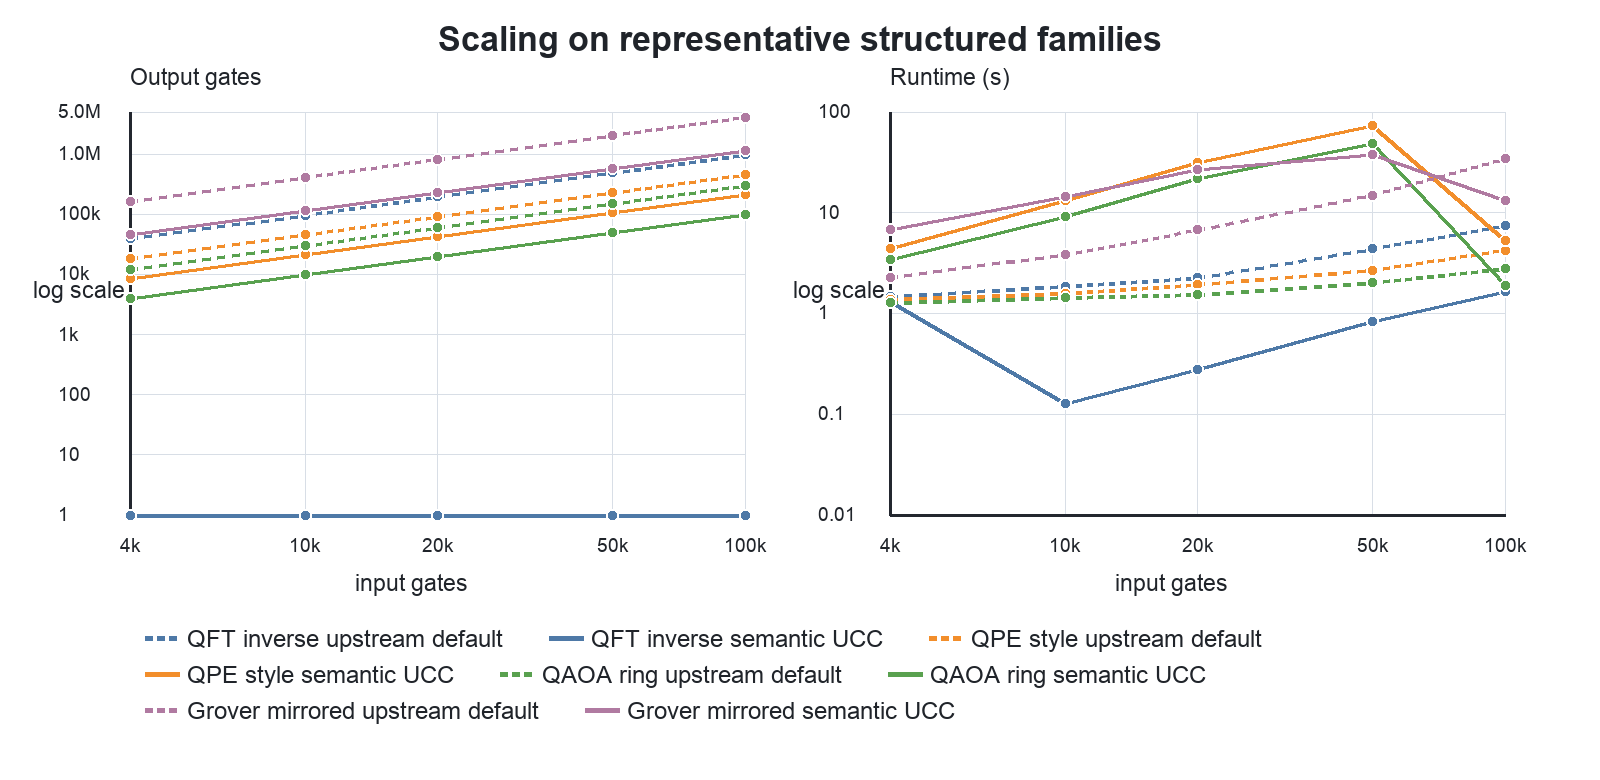
\includegraphics[width=\textwidth]{figures/scaling_plot.png}}{\fbox{\parbox{0.9\textwidth}{\centering\vspace{2em}Missing file: \texttt{figures/scaling\_plot.png}.\vspace{2em}}}}
\caption{Scaling behavior on representative structured families. Left: output gate count versus input gate count for upstream default (baseline UCC) and the semantic UCC artifact. Right: runtime versus input gate count. The semantic path preserves clear quality advantages across scale, while runtime behavior remains family-dependent.}
\label{fig:scaling}
\end{figure*}

\subsection{Scaling and Ablation}

The main scaling trends are summarized in \cref{fig:scaling}. The size sweep
covers $4$k, $10$k, $20$k, $50$k, and $100$k inputs for QFT-inverse,
QPE-style, QAOA-ring, and mirrored-Grover families; the QAOA-ring block uses
20 qubits. The most important
observations are stable quality behavior across scale and improving
repeated-family runtime once the semantic representation and dispatch controller are
enabled. The method is most effective on exact or highly repeated structure:
\texttt{qft\_inverse} remains maximally strong across all tested sizes,
\texttt{qpe\_style} remains a strong positive fixed-basis case,
\texttt{qaoa\_ring} consistently avoids UCC inflation, and the mirrored-Grover
family continues to match Qiskit quality at $100$k while remaining
more expensive. Direct spot checks on the semantic artifact give
\texttt{qpe\_style} $=82{,}200$ gates at $50$k in $2.504$ s and $164{,}400$
gates at $100$k in $4.636$ s, reflecting the phase-ladder plus
repeated-run controller improvements.

The non-monotonic semantic runtime between the $20$k and $50$k points is a
dispatch effect visible in the implementation, not an inferred hardware
effect. The 20,000-gate full-preset limit
\path{_MAX_FULL_PRESET_REFERENCE_SIZE} allows the 19,998-gate input to enter
the full preset-reference comparison,
whereas the 49,998-gate input exceeds that threshold and uses the cheaper
repeated-prefix/hierarchical route. The corresponding canonical witness
runtimes are 28.314~s and 20.934~s. This threshold explains the local drop;
it is not evidence of asymptotically decreasing compilation time.

The ablation picture is narrow. The dominant practical component is
conservative candidate control on recoverability-sensitive families, most
clearly on the 10,000-input-gate \texttt{qaoa\_ring} row, where the full configuration returns
$10{,}000$ gates while the no-candidate-selection variant returns $30{,}055$.
By contrast, \texttt{qft\_inverse}, \texttt{qft\_control},
\texttt{qpe\_style}, and \texttt{grover\_mirrored} are less sensitive to the
removal of individual structural rules. This reinforces the paper's current
framing: the main contribution is a bounded semantic representation and
dispatch controller that preserve recoverability before flat materialization,
rather than a single local identity.


\bibliography{references}

\end{document}
